% Template for PLoS Supplementary Material
% Version 3.6 Aug 2022

\documentclass[10pt,letterpaper]{article}
\usepackage[top=0.85in,left=2.75in,footskip=0.75in]{geometry}
\usepackage{amsmath,amssymb}
\usepackage{changepage}
\usepackage{textcomp,marvosym}
\usepackage{cite}
\usepackage{nameref,hyperref}
\usepackage[right]{lineno}
\usepackage[nopatch=eqnum]{microtype}
\usepackage{float}
\usepackage[section]{placeins}
\DisableLigatures[f]{encoding = *, family = * }
\usepackage[table]{xcolor}
\usepackage{array}
\usepackage{lastpage,fancyhdr,graphicx,epstopdf}
\pagestyle{fancy}
\fancyhf{}
\rfoot{\thepage/\pageref{LastPage}}
\renewcommand{\headrulewidth}{0pt}
\renewcommand{\footrule}{\hrule height 2pt \vspace{2mm}}
\fancyheadoffset[L]{2.25in}
\fancyfootoffset[L]{2.25in}
\lfoot{\today}
\raggedright
\setlength{\parindent}{0.5cm}
\textwidth 5.25in 
\textheight 8.75in
\usepackage[aboveskip=1pt,labelfont=bf,labelsep=period,justification=raggedright,singlelinecheck=off]{caption}
\renewcommand{\figurename}{Fig}

\begin{document}
\vspace*{0.2in}

\begin{flushleft}
{\Large
\textbf\newline{Supporting Information}
}
\newline
\\
Investigating Audience Preferences Within the Hybrid Competitive-Comedic Format of Taskmaster UK
\newline
\\
David H. Silver\textsuperscript{1*}
\\
\bigskip
\textbf{1} Remiza AI\\
\bigskip
* Corresponding author: david@remiza.ai
\end{flushleft}

\section*{Supporting information}

\paragraph*{S1 Fig.}
\label{S1_Fig}
{\bf Sentiment Variability Across Episodes.} 
Box plots showing the distribution of each sentiment category across the full 154-episode corpus. While mean levels remain stable, awkwardness exhibits a broader distribution in later series.

\begin{figure}[!h]
\centering
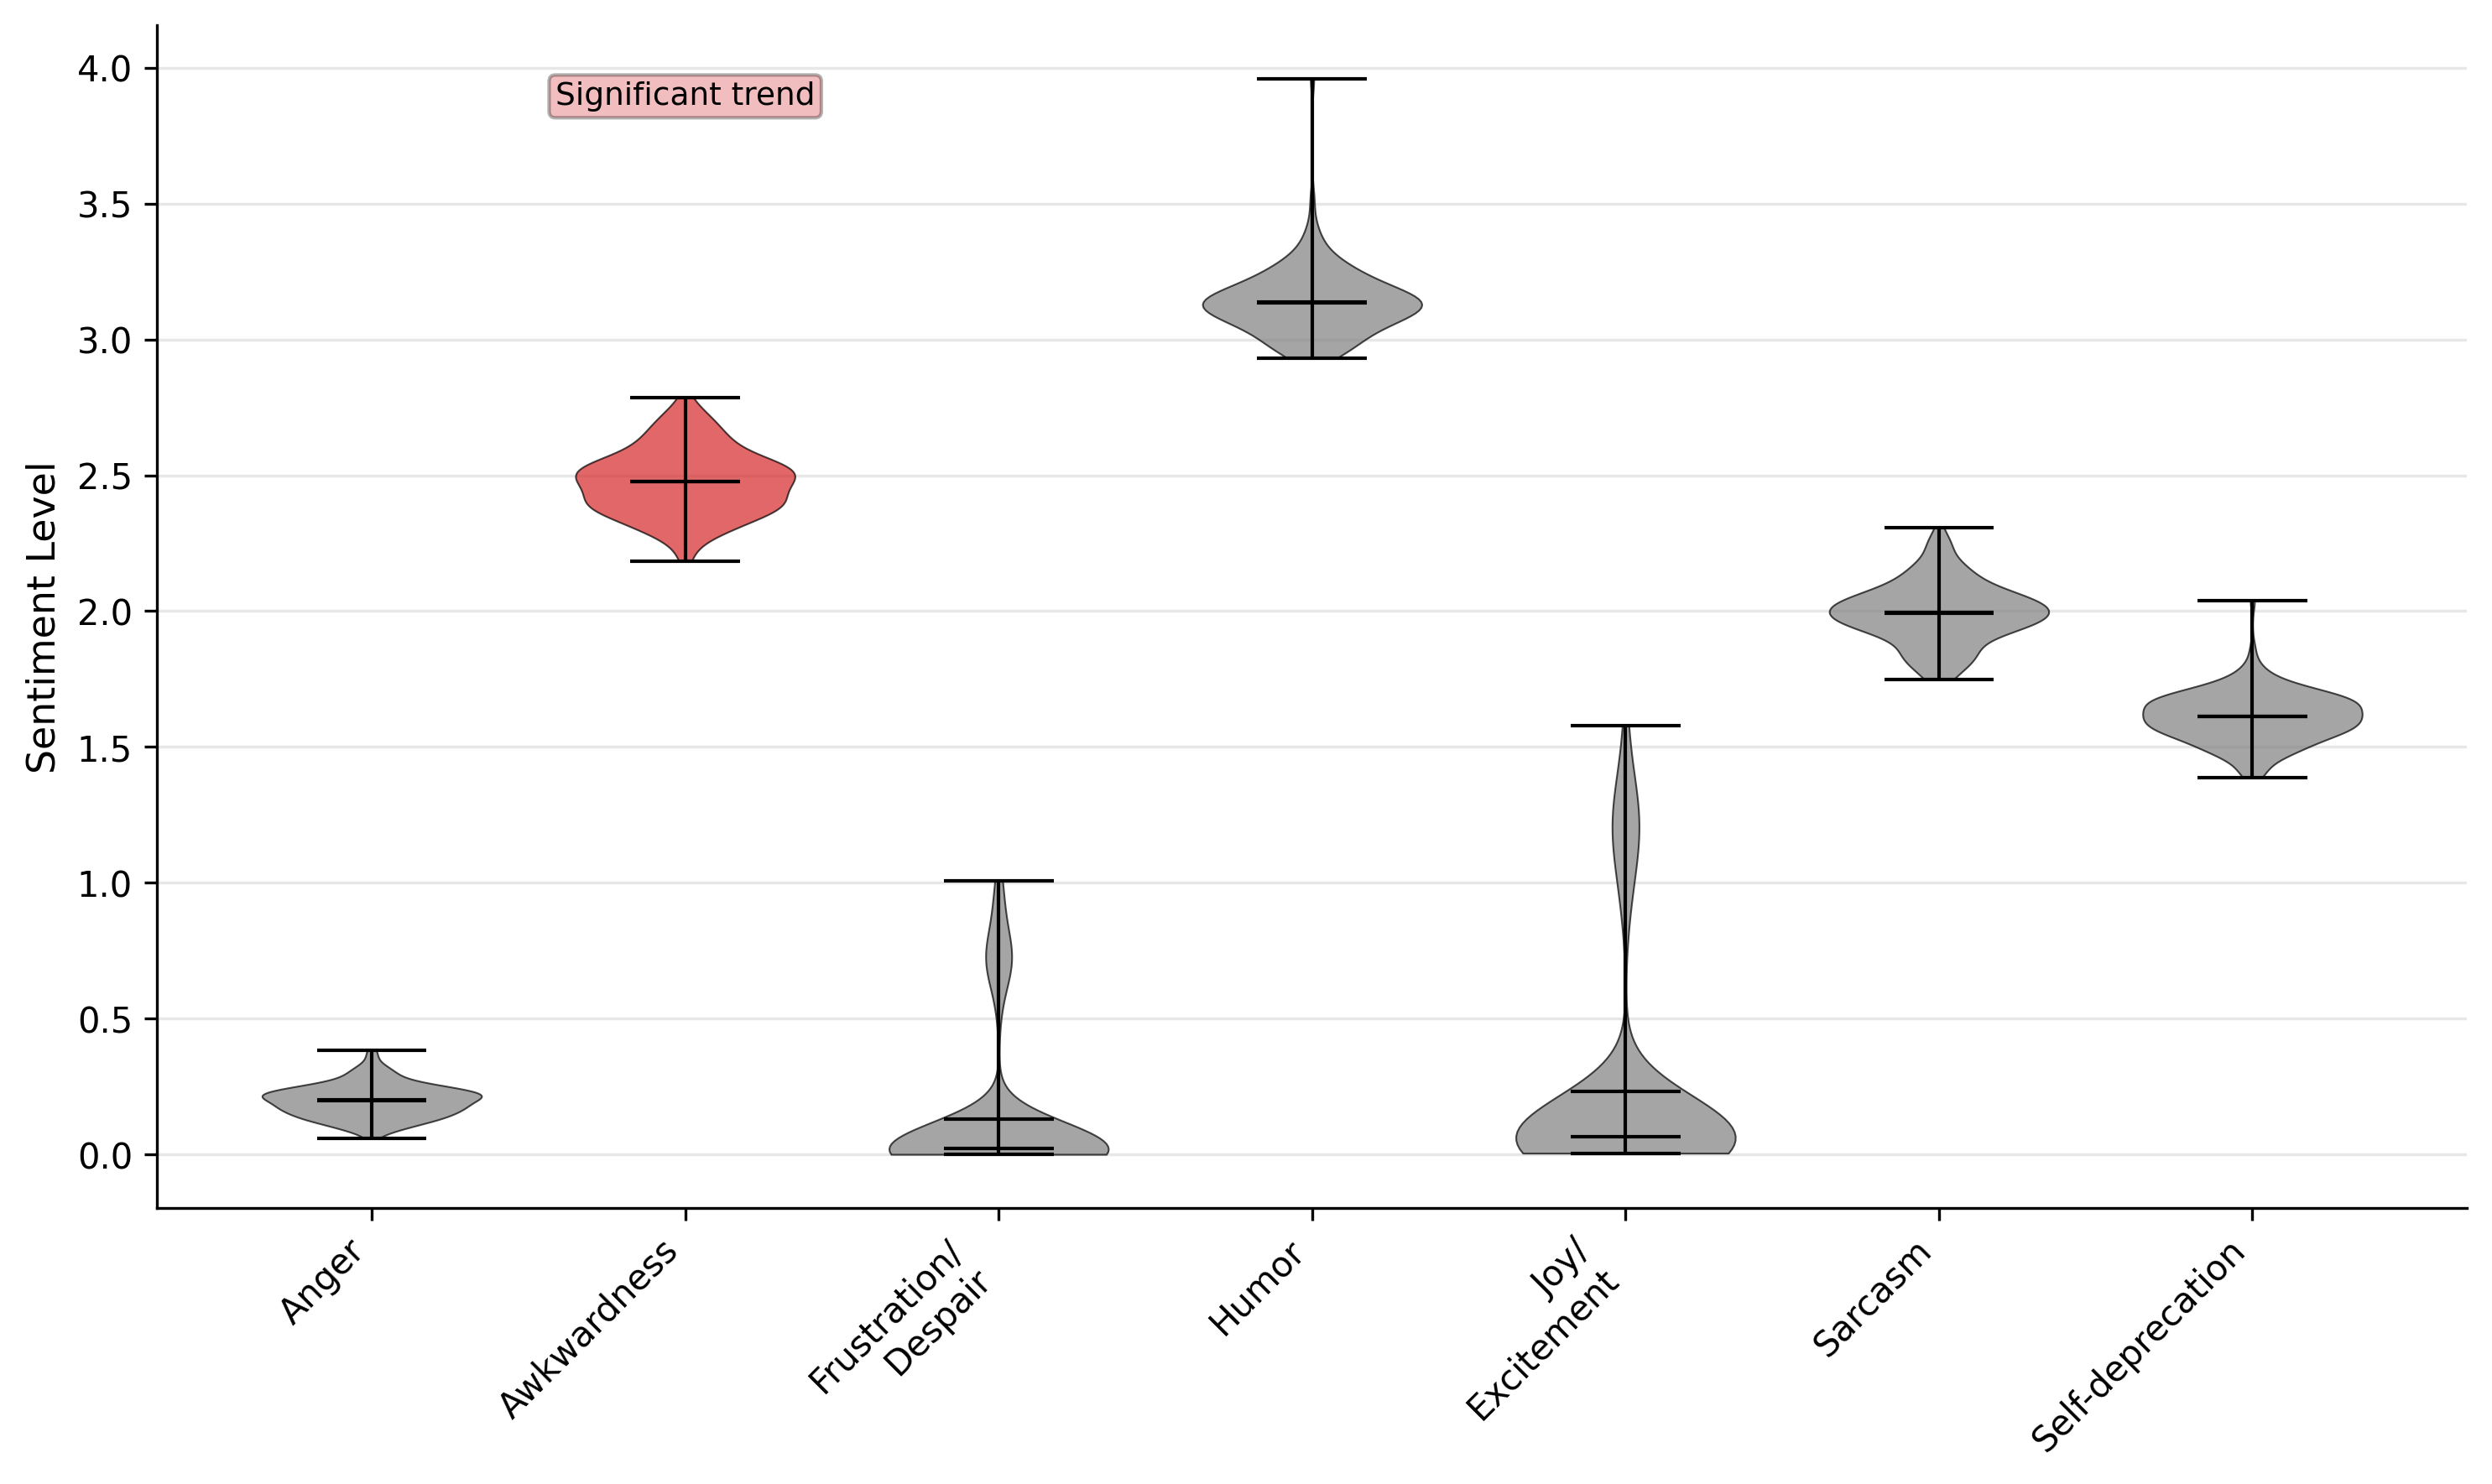
\includegraphics[width=\linewidth]{figures/supplementary/figure7b.png}
\end{figure}
\FloatBarrier

\paragraph*{S2 Fig.}
\label{S2_Fig}
{\bf Feature–Rating Correlation Histogram.} 
Distribution of Pearson correlation coefficients between 45 episode-level features and IMDb ratings. Sentiment and contestant attributes dominate the upper tail, while task features are near zero.

\begin{figure}[!h]
\centering
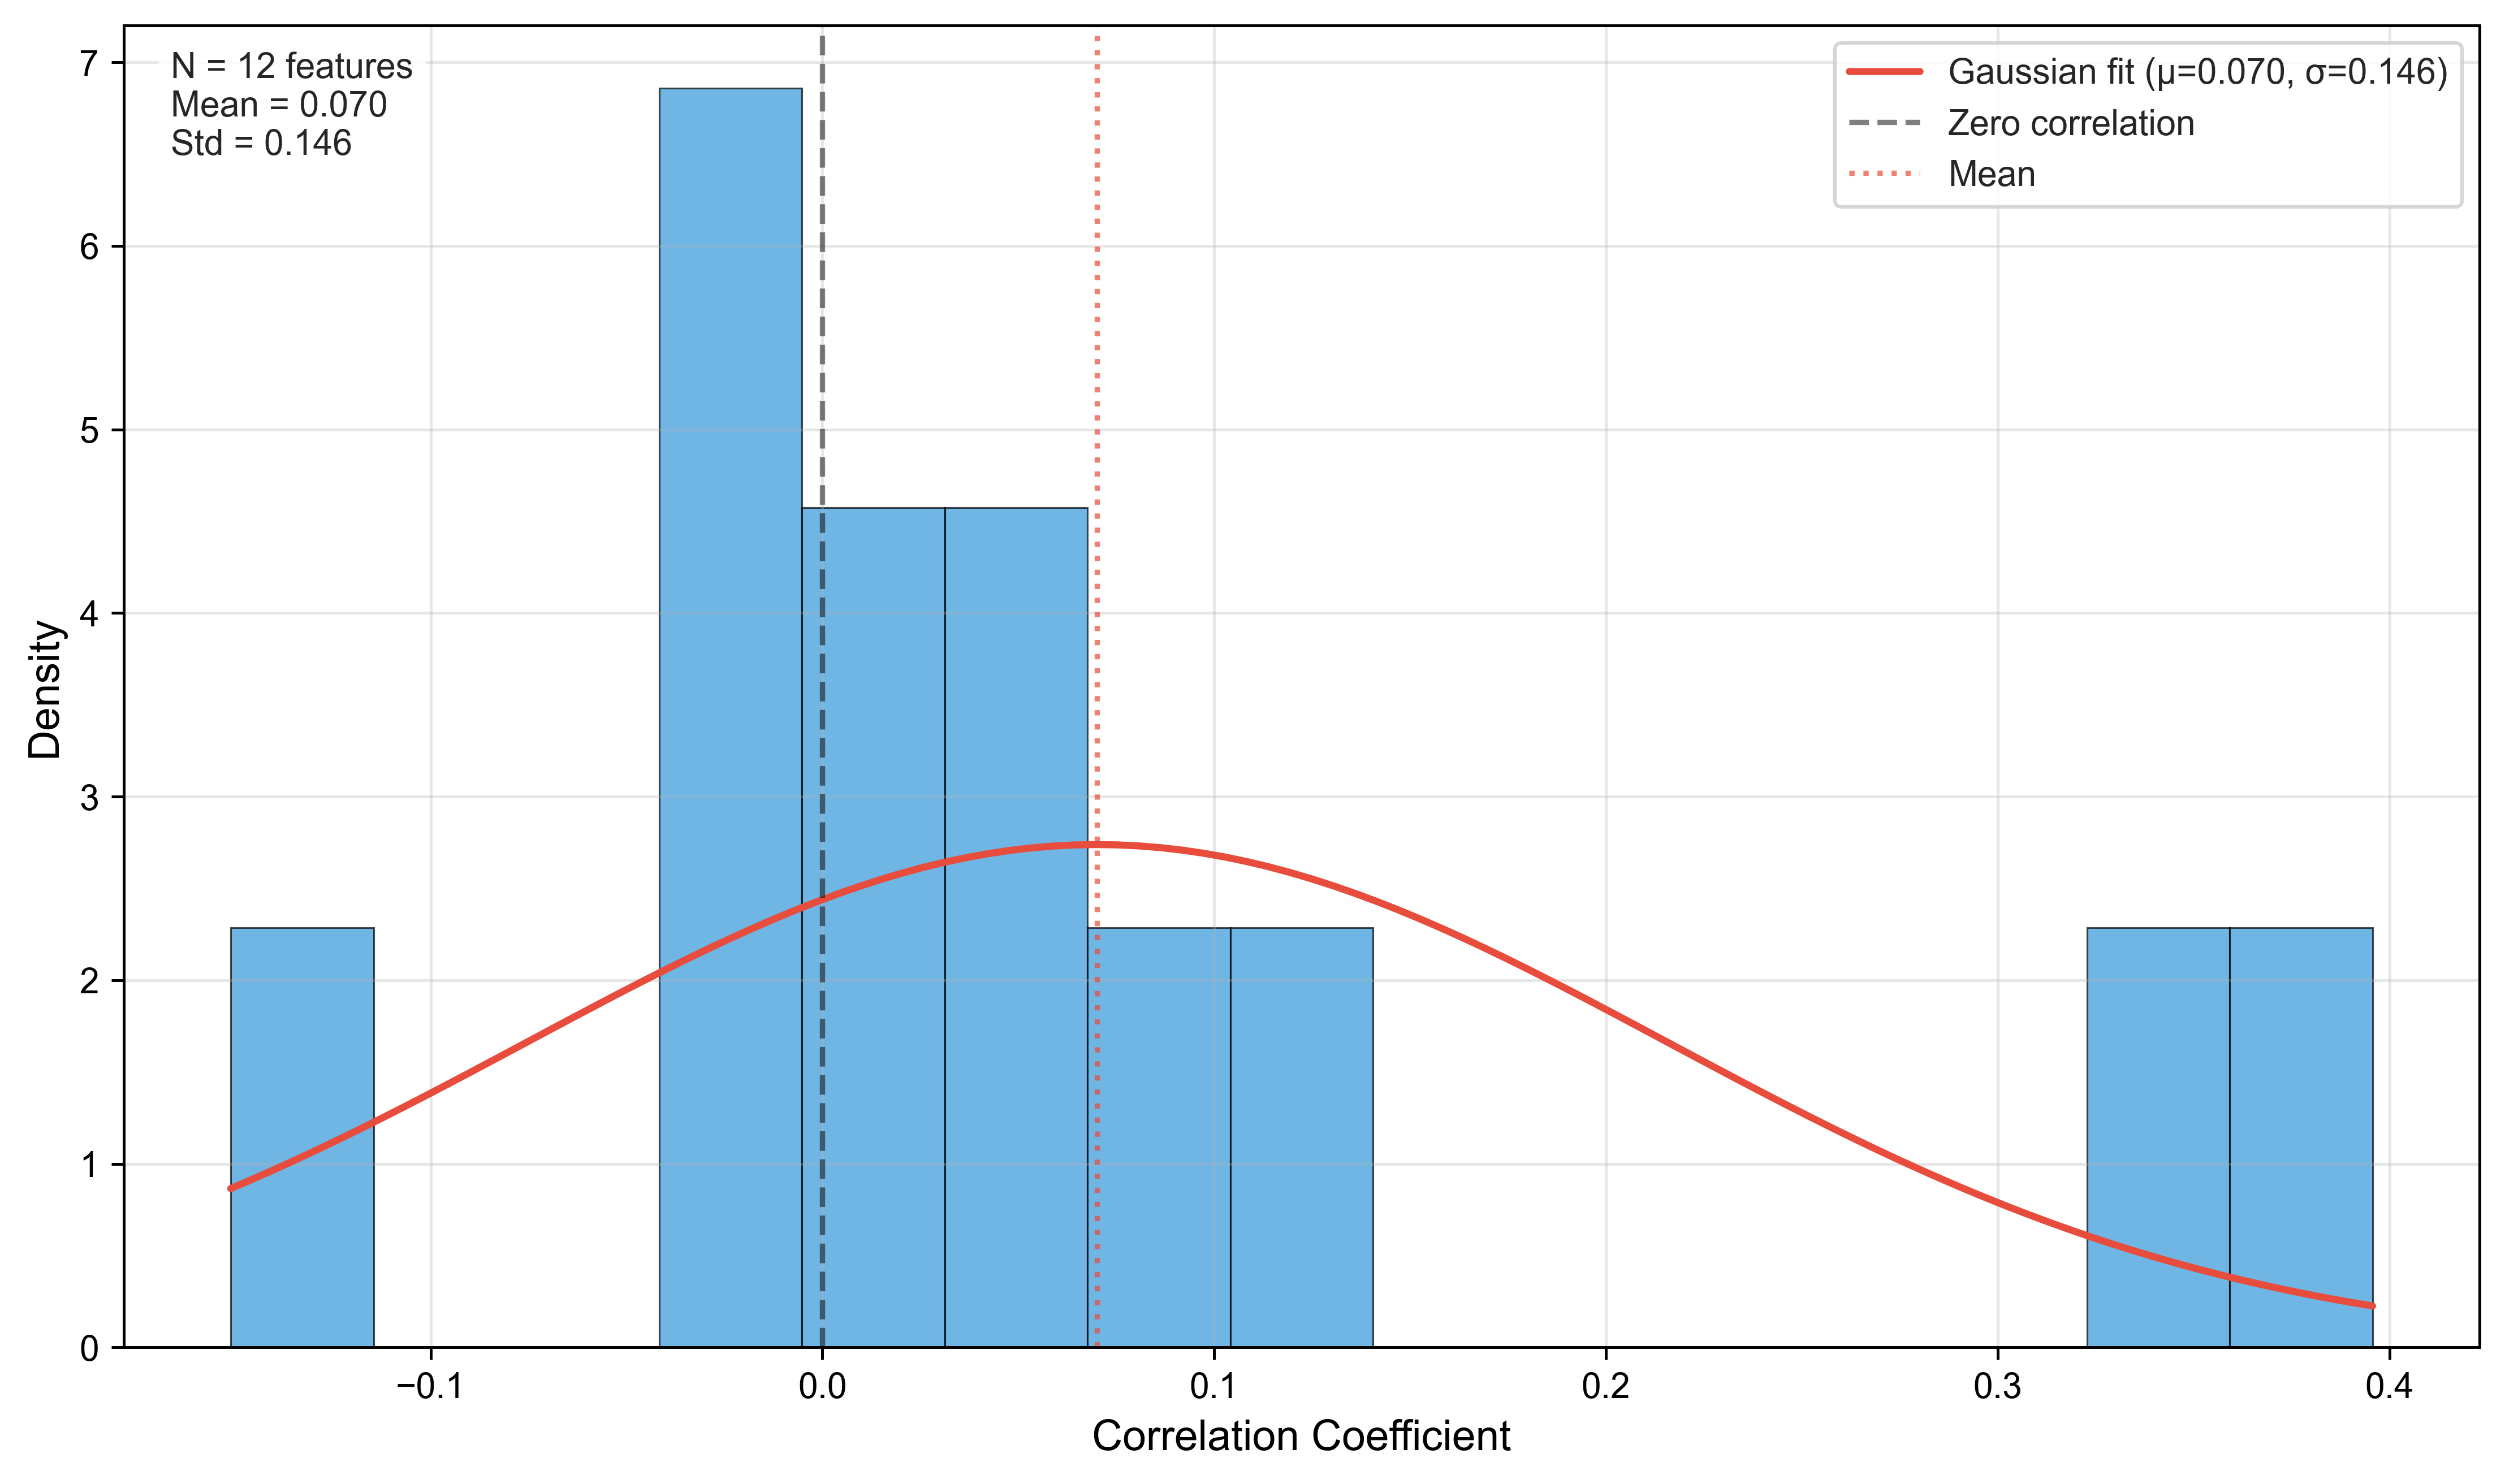
\includegraphics[width=\linewidth]{figures/supplementary/figure8b_raw_correlations.png}
\end{figure}
\FloatBarrier

\paragraph*{S3 Fig.}
\label{S3_Fig}
{\bf Series-Level Deep Dive Visualizations.}
One-page summaries of all 18 Taskmaster UK series. Each page includes two panels: cumulative contestant score progression (top) and per-task rank evolution (bottom). These visualizations support archetype consistency and highlight turning points in series narratives.

\begin{figure}[!h]
\centering
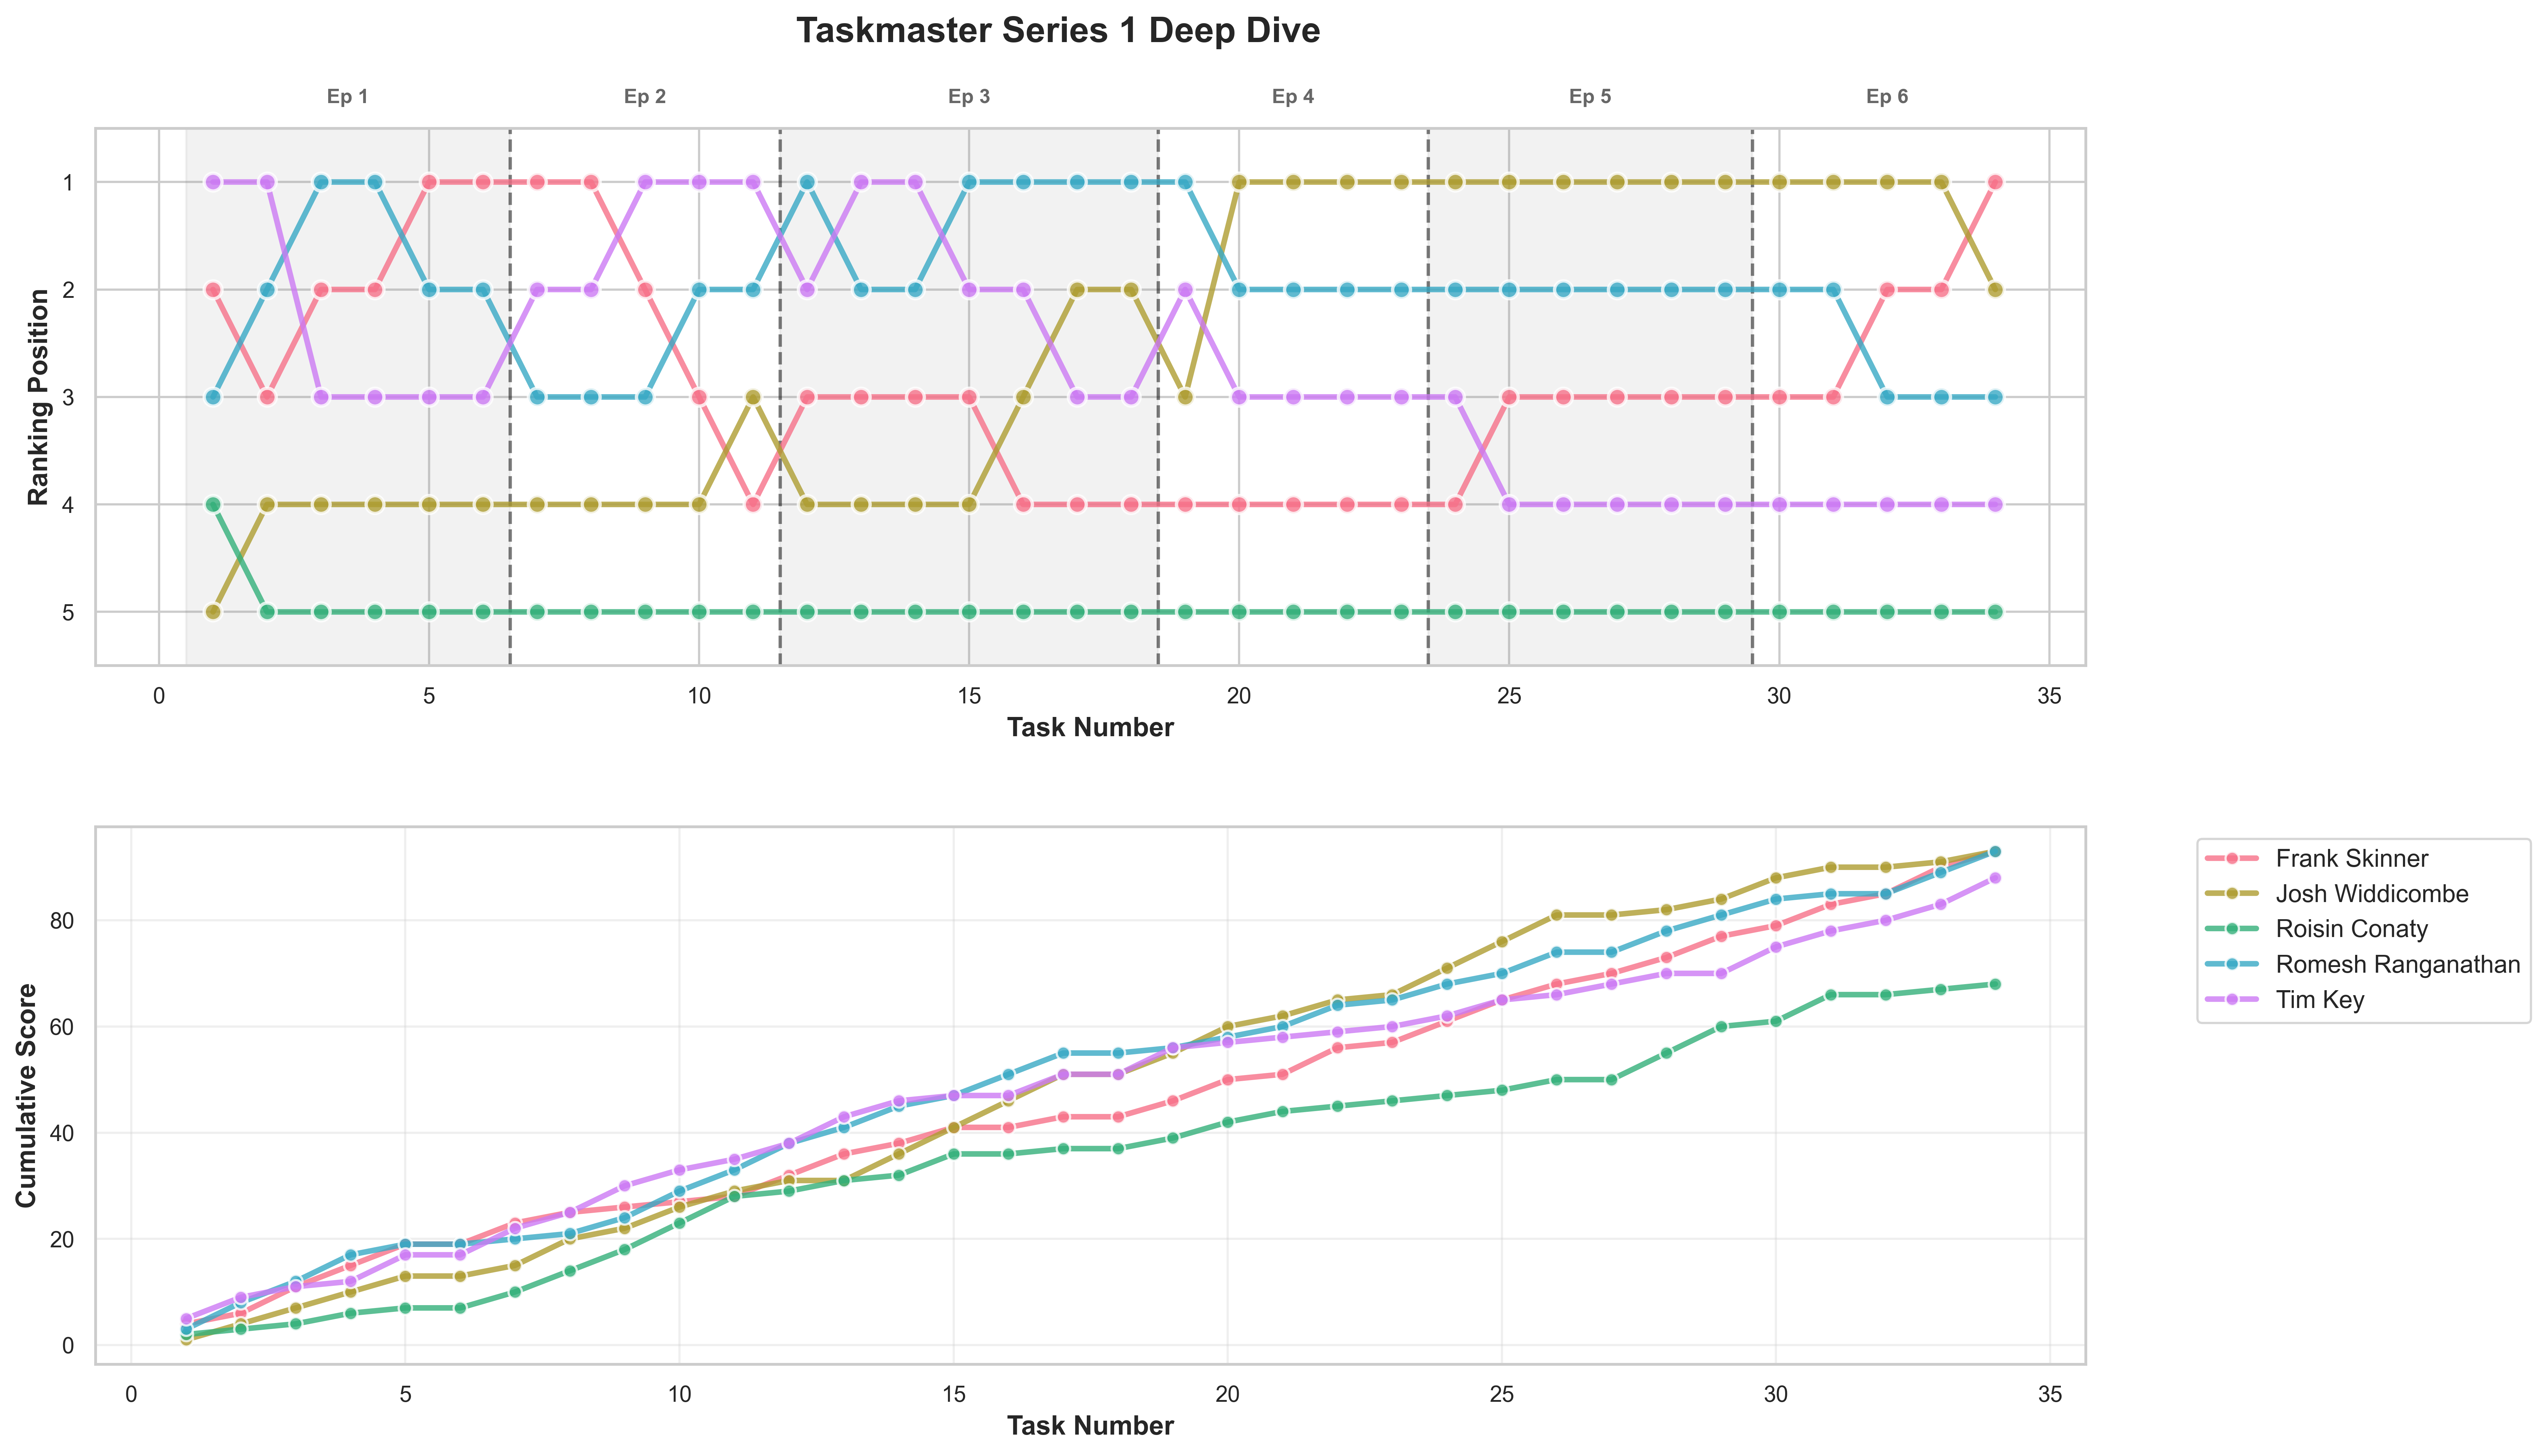
\includegraphics[width=\linewidth]{figures/supplementary/series_1_deep_dive.png}
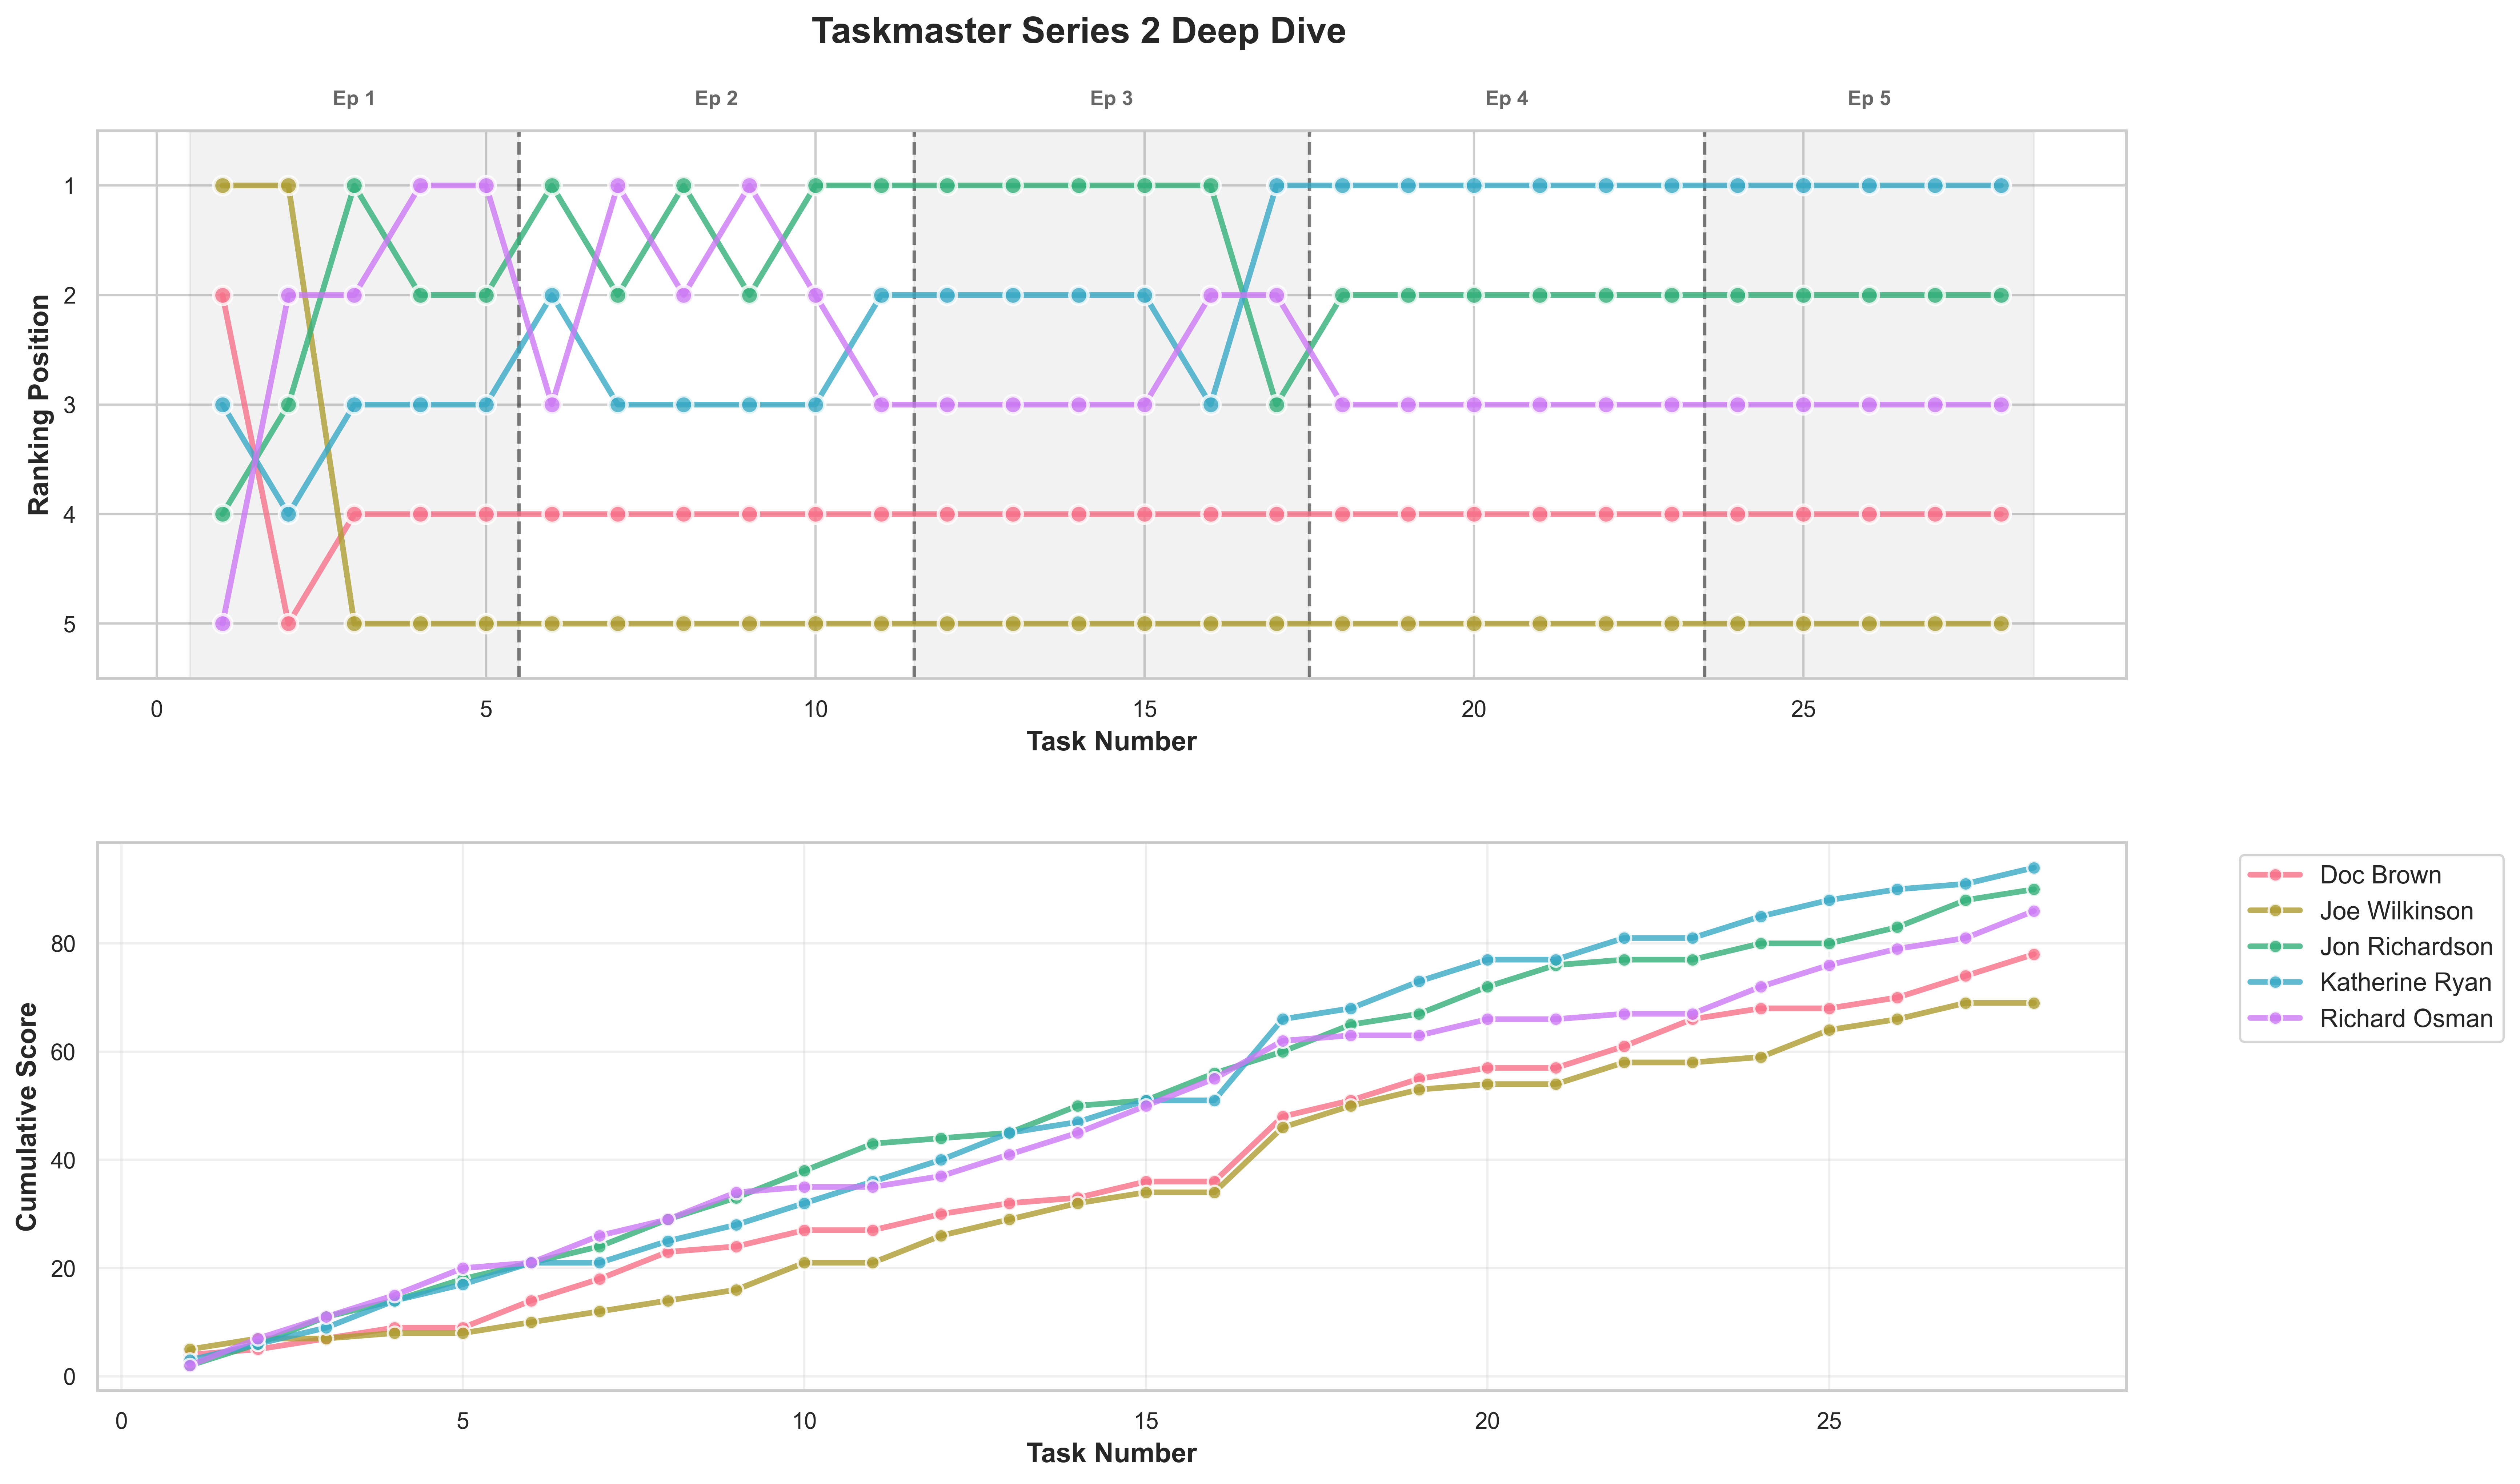
\includegraphics[width=\linewidth]{figures/supplementary/series_2_deep_dive.png}
\end{figure}
\FloatBarrier
\clearpage

\begin{figure}[!h]
\centering
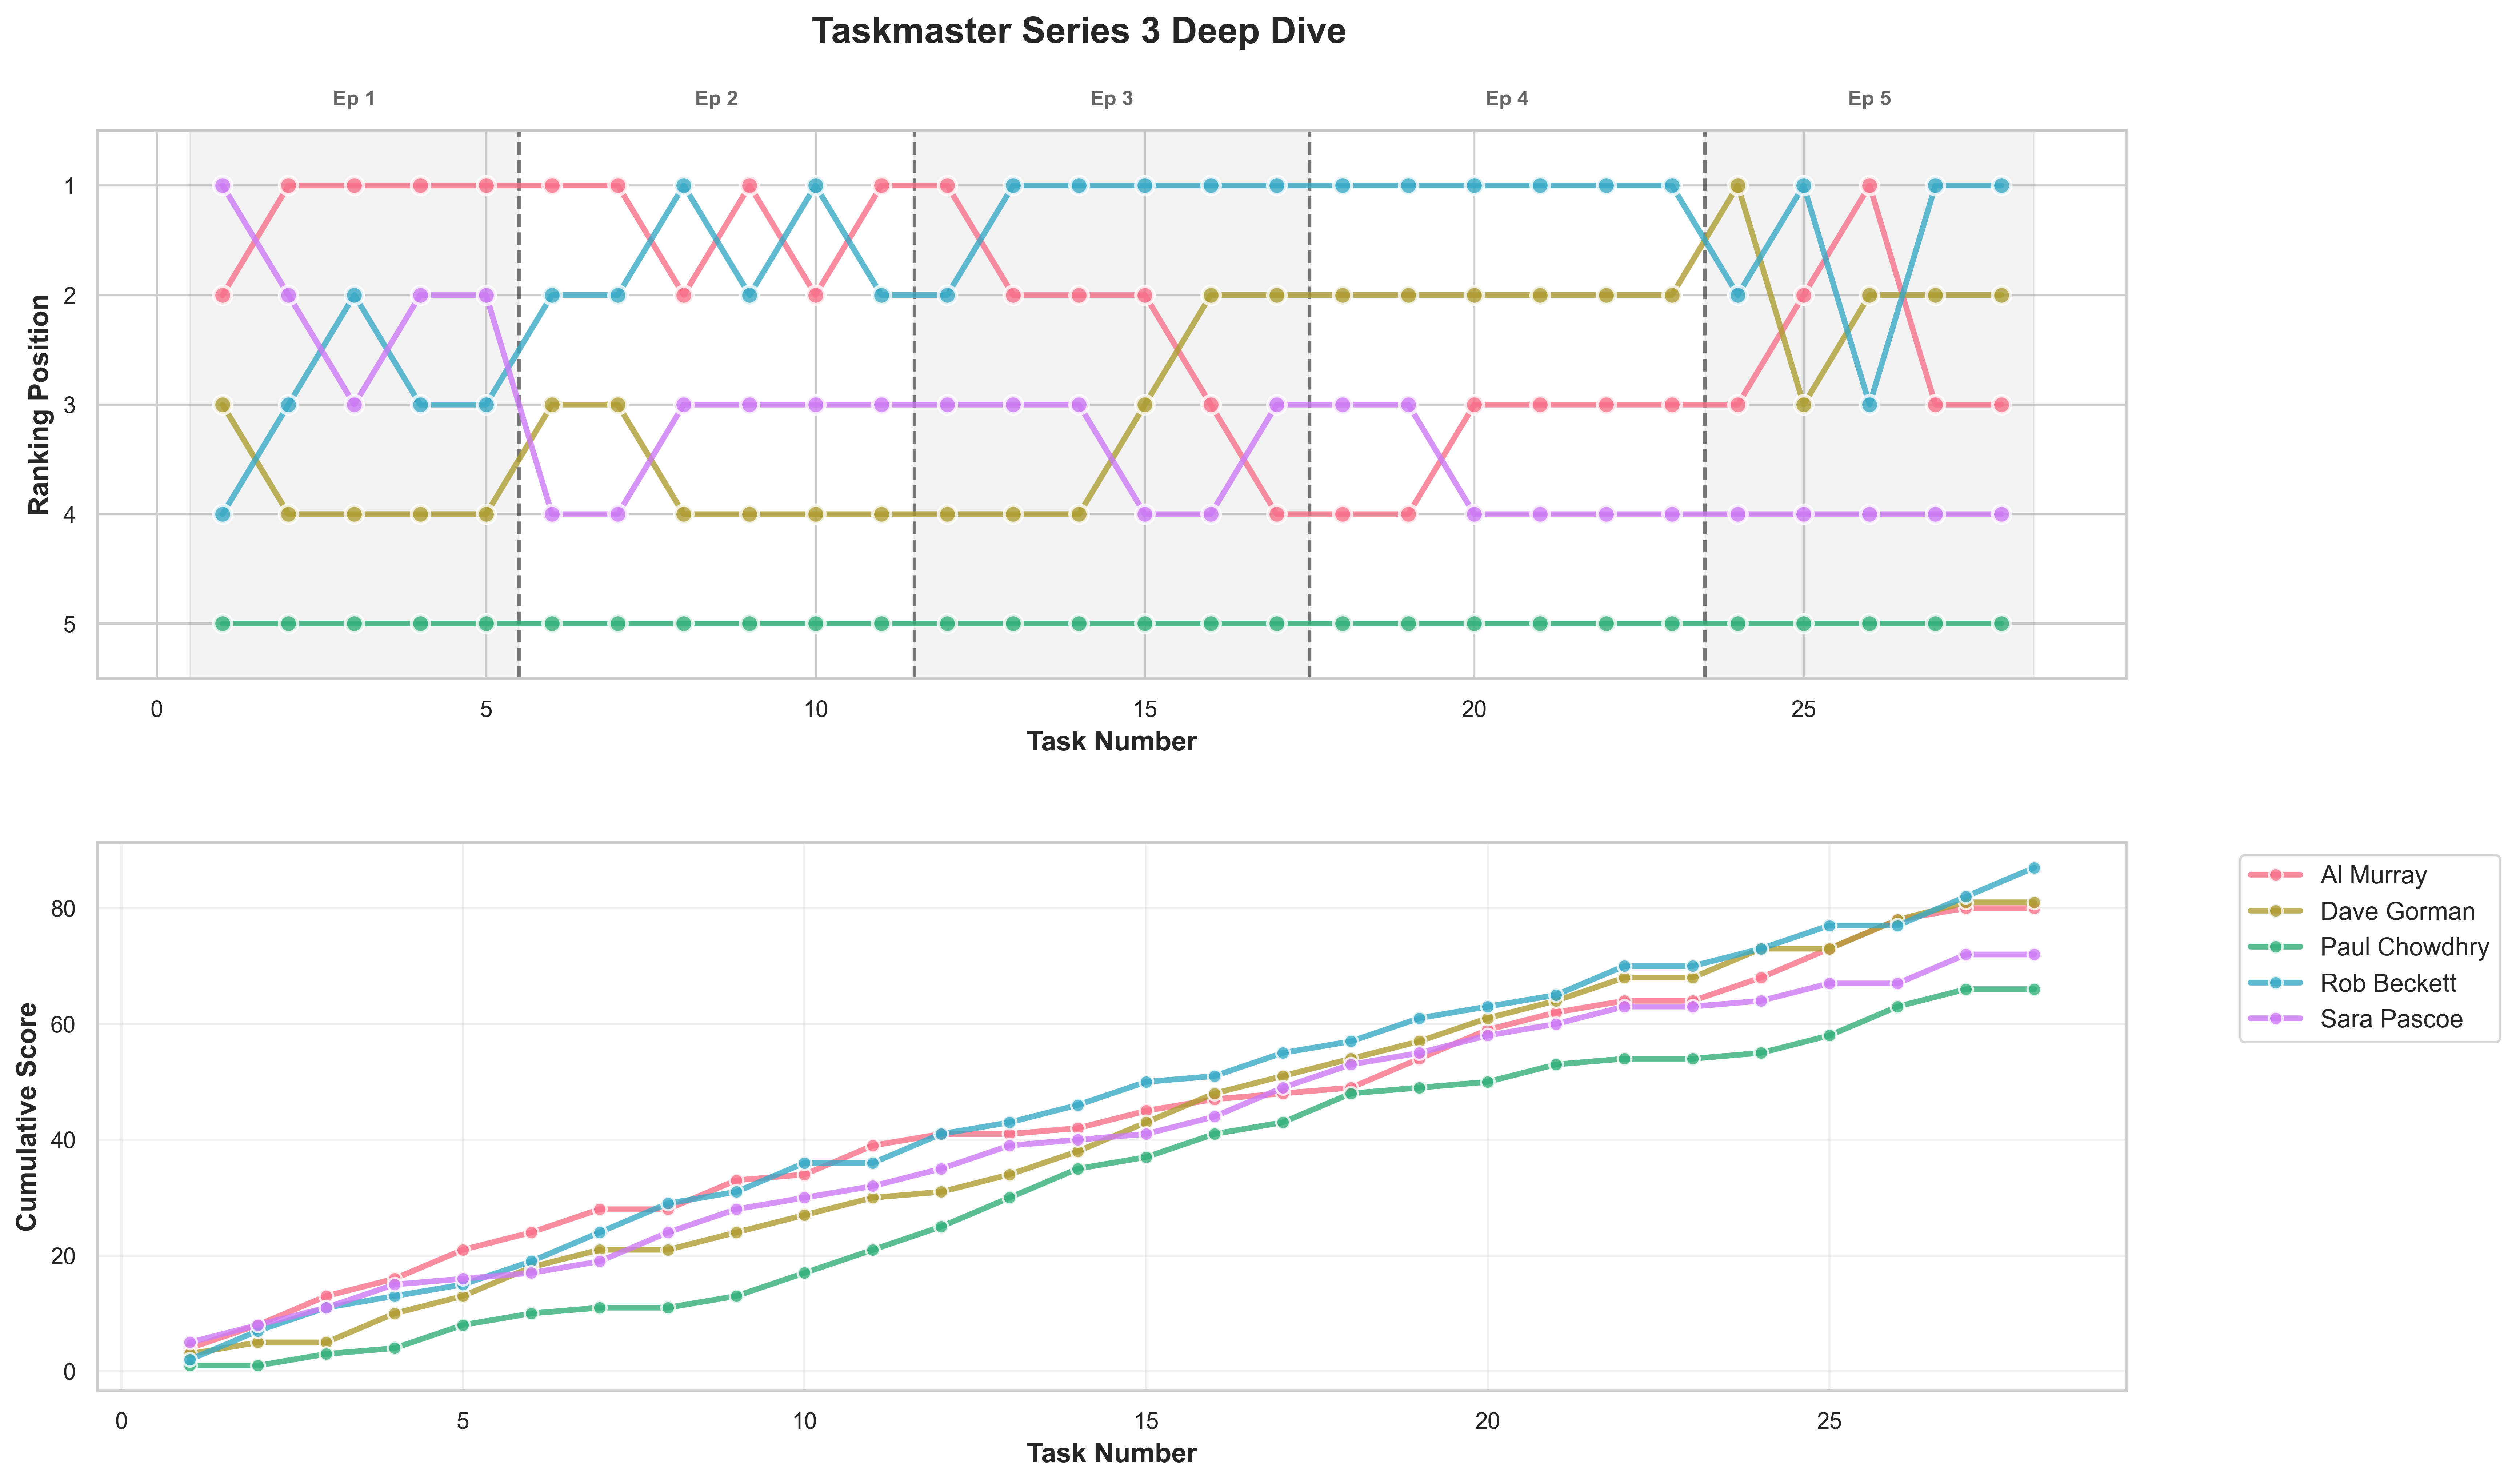
\includegraphics[width=\linewidth]{figures/supplementary/series_3_deep_dive.png}
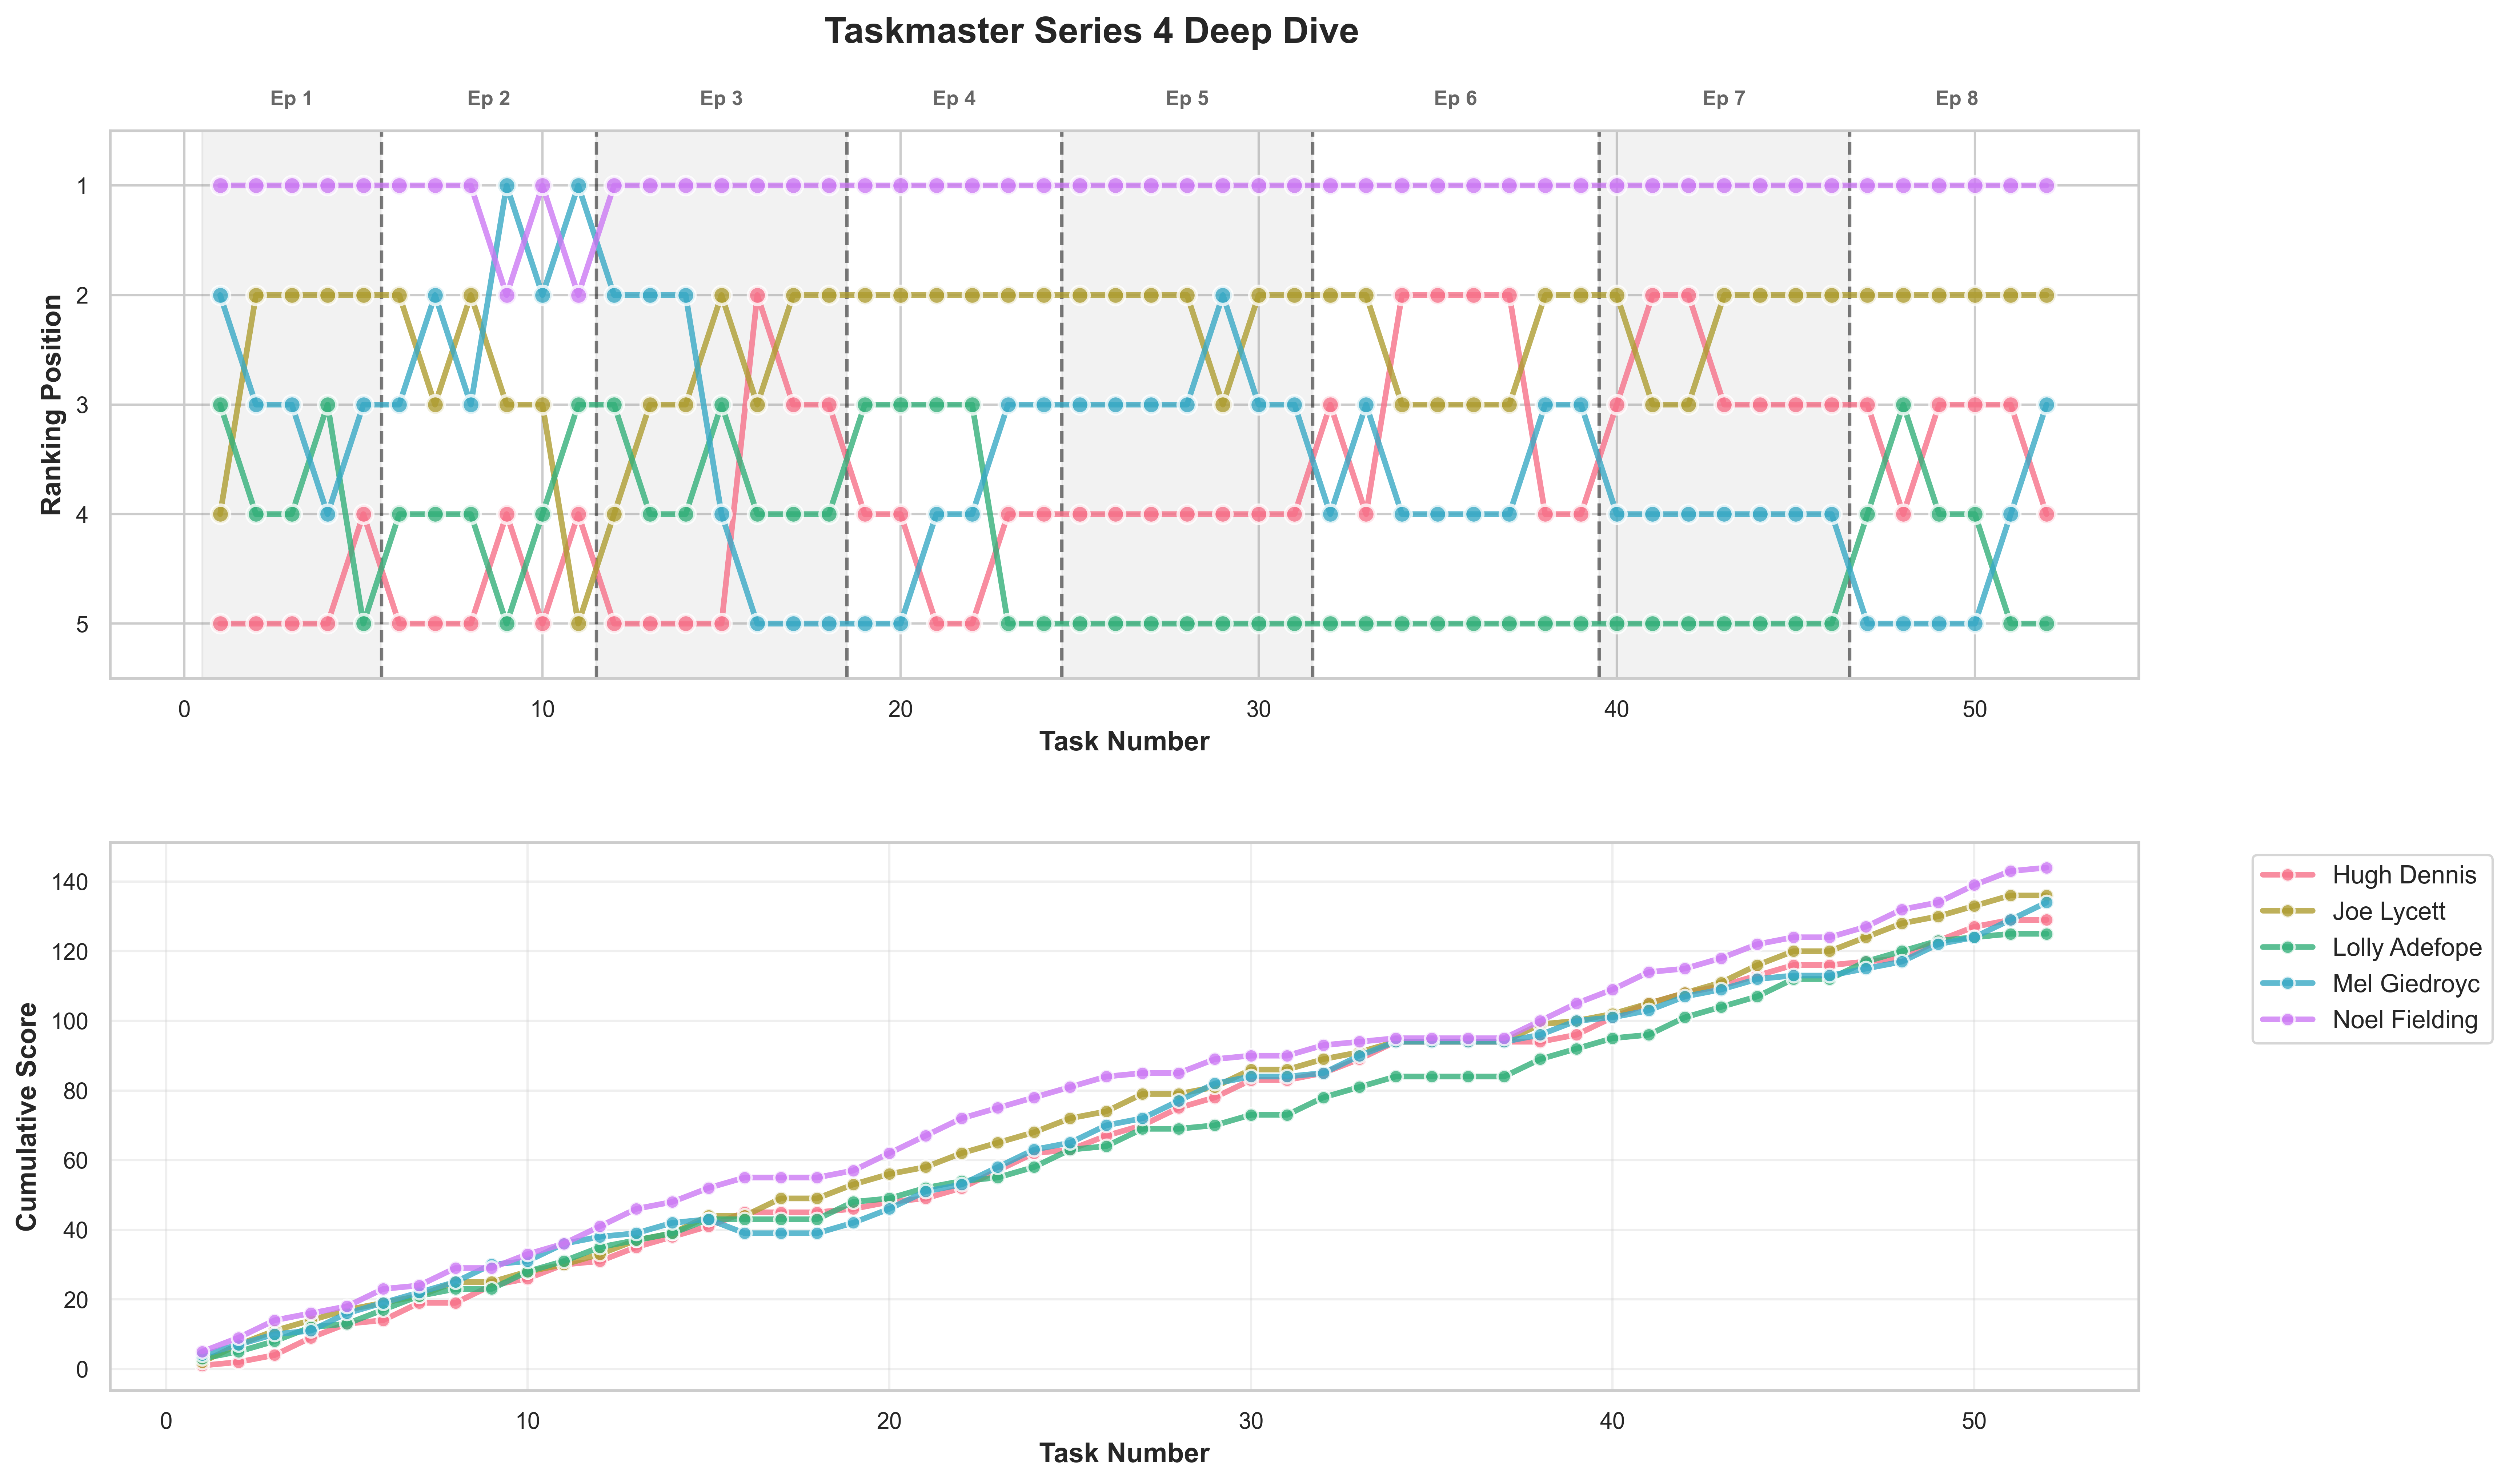
\includegraphics[width=\linewidth]{figures/supplementary/series_4_deep_dive.png}
\end{figure}
\FloatBarrier
\clearpage

\begin{figure}[!h]
\centering
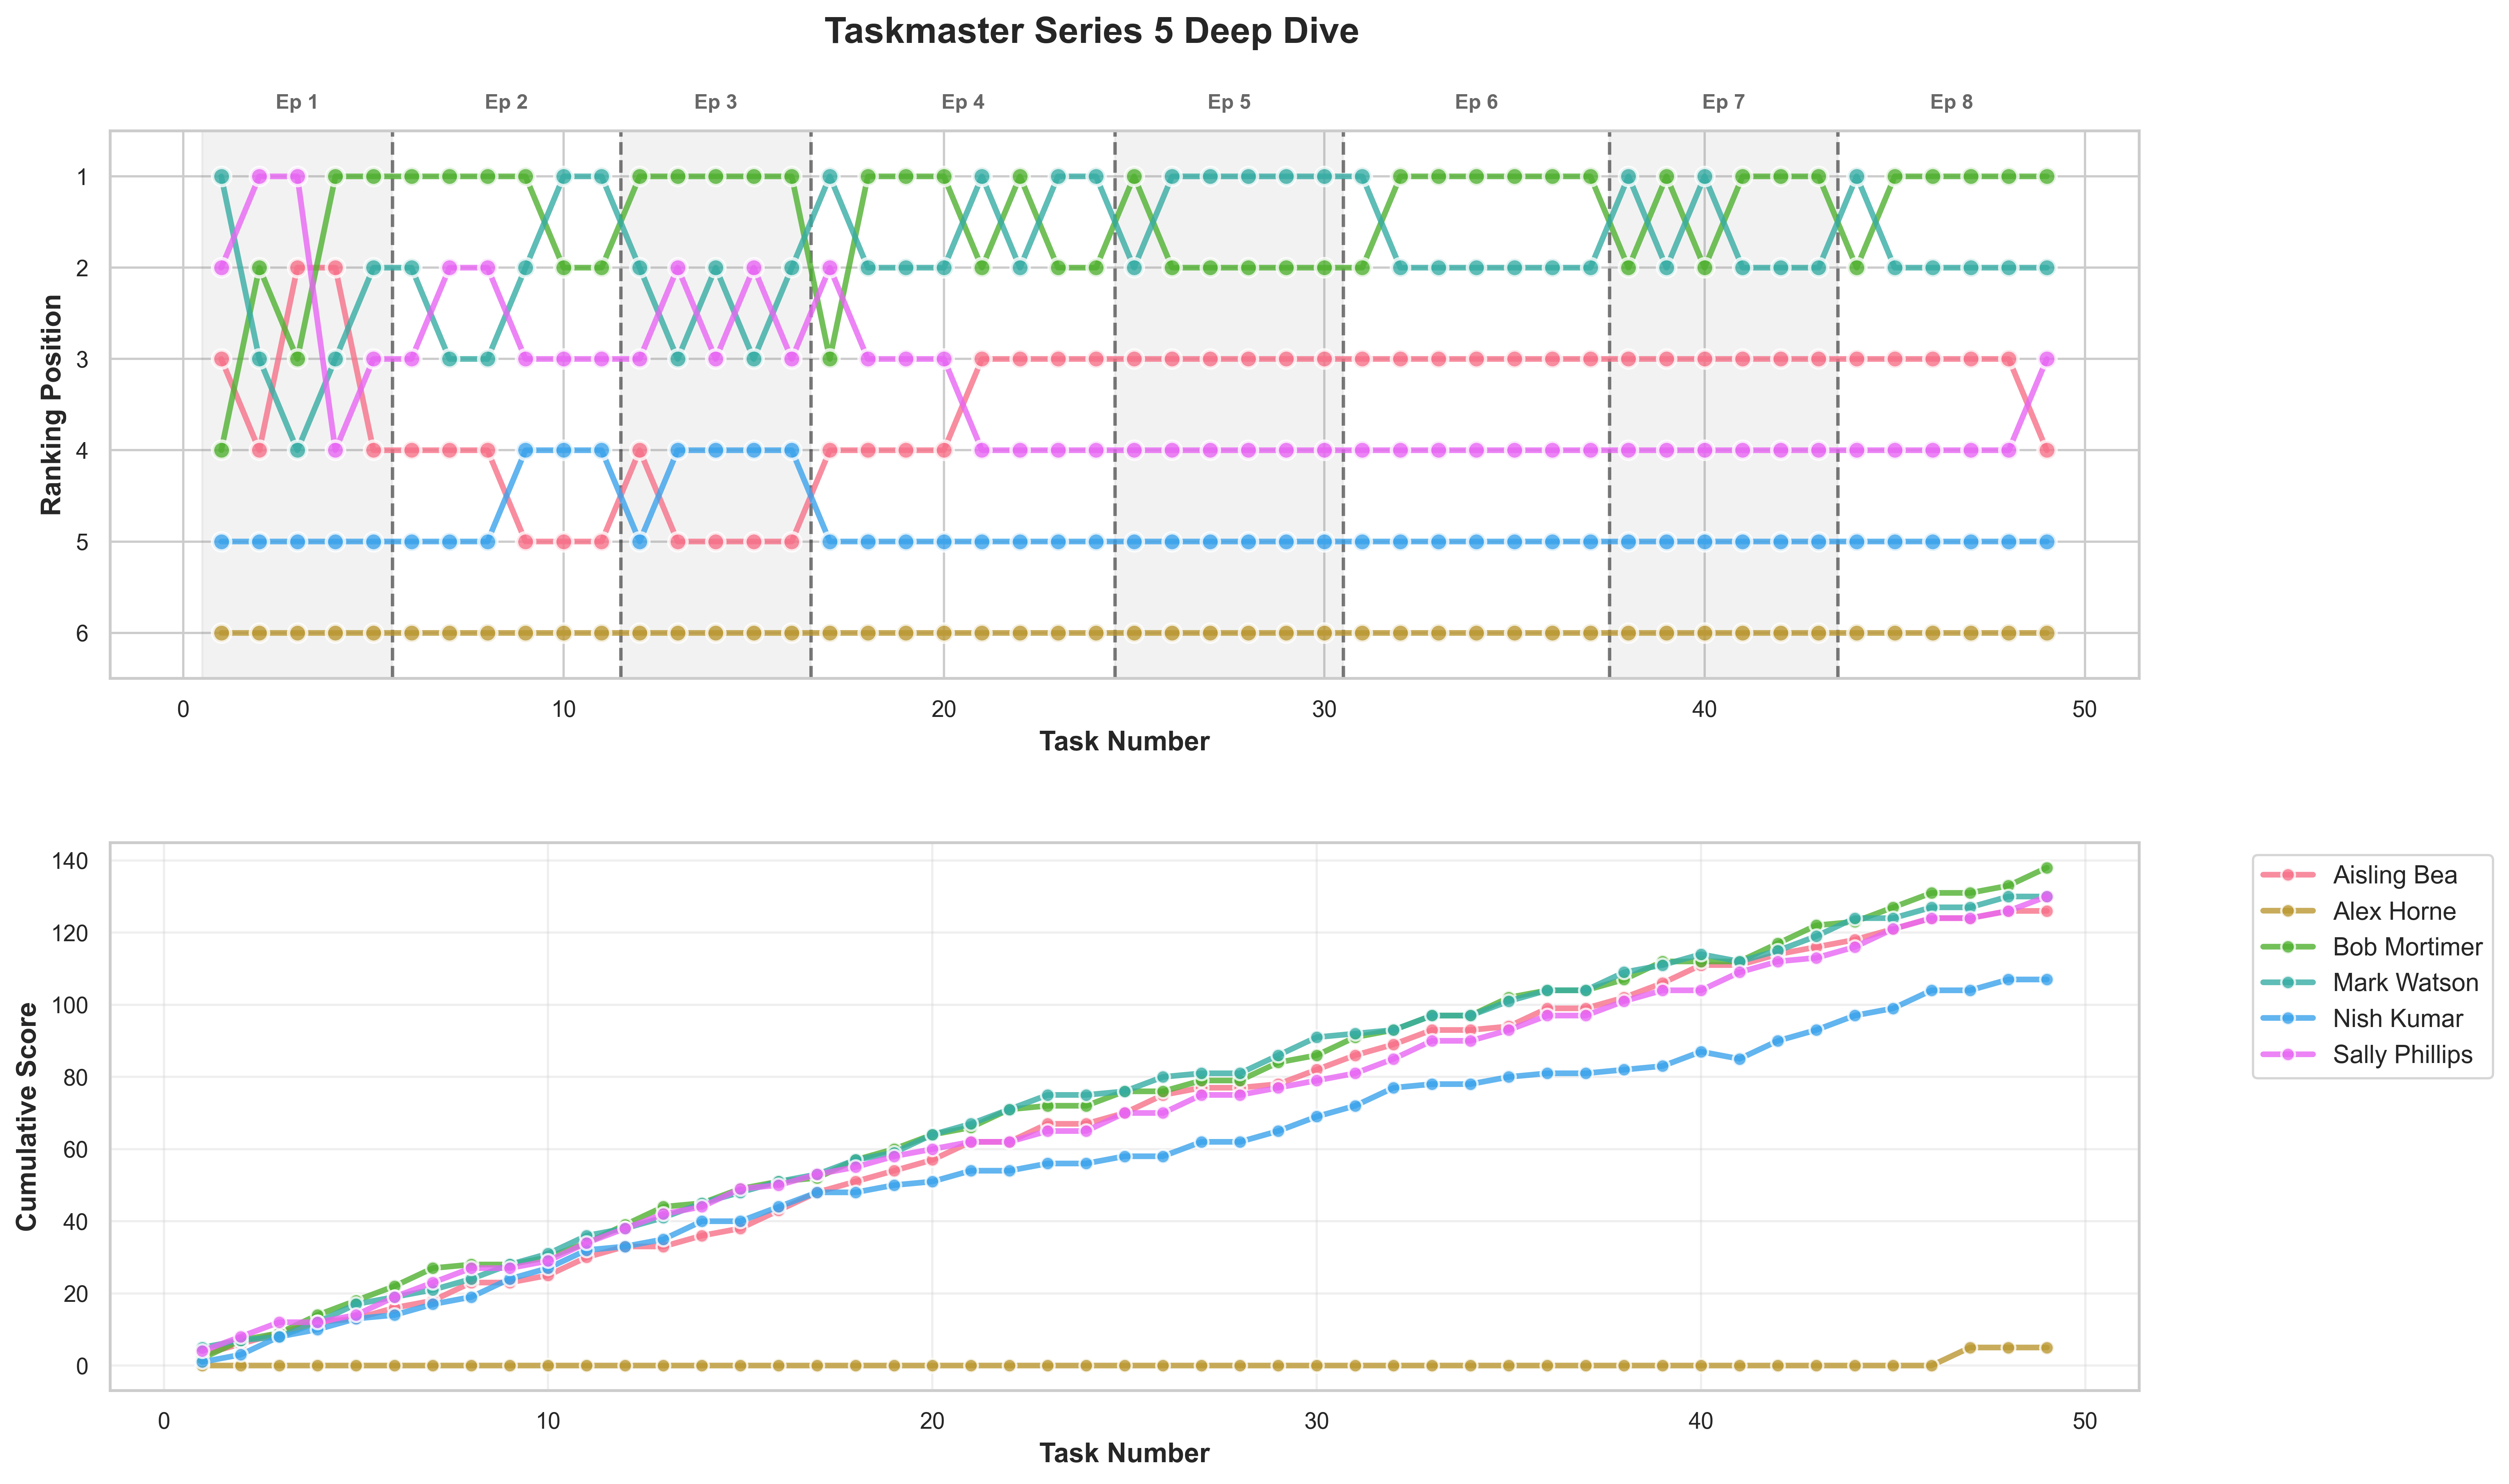
\includegraphics[width=\linewidth]{figures/supplementary/series_5_deep_dive.png}
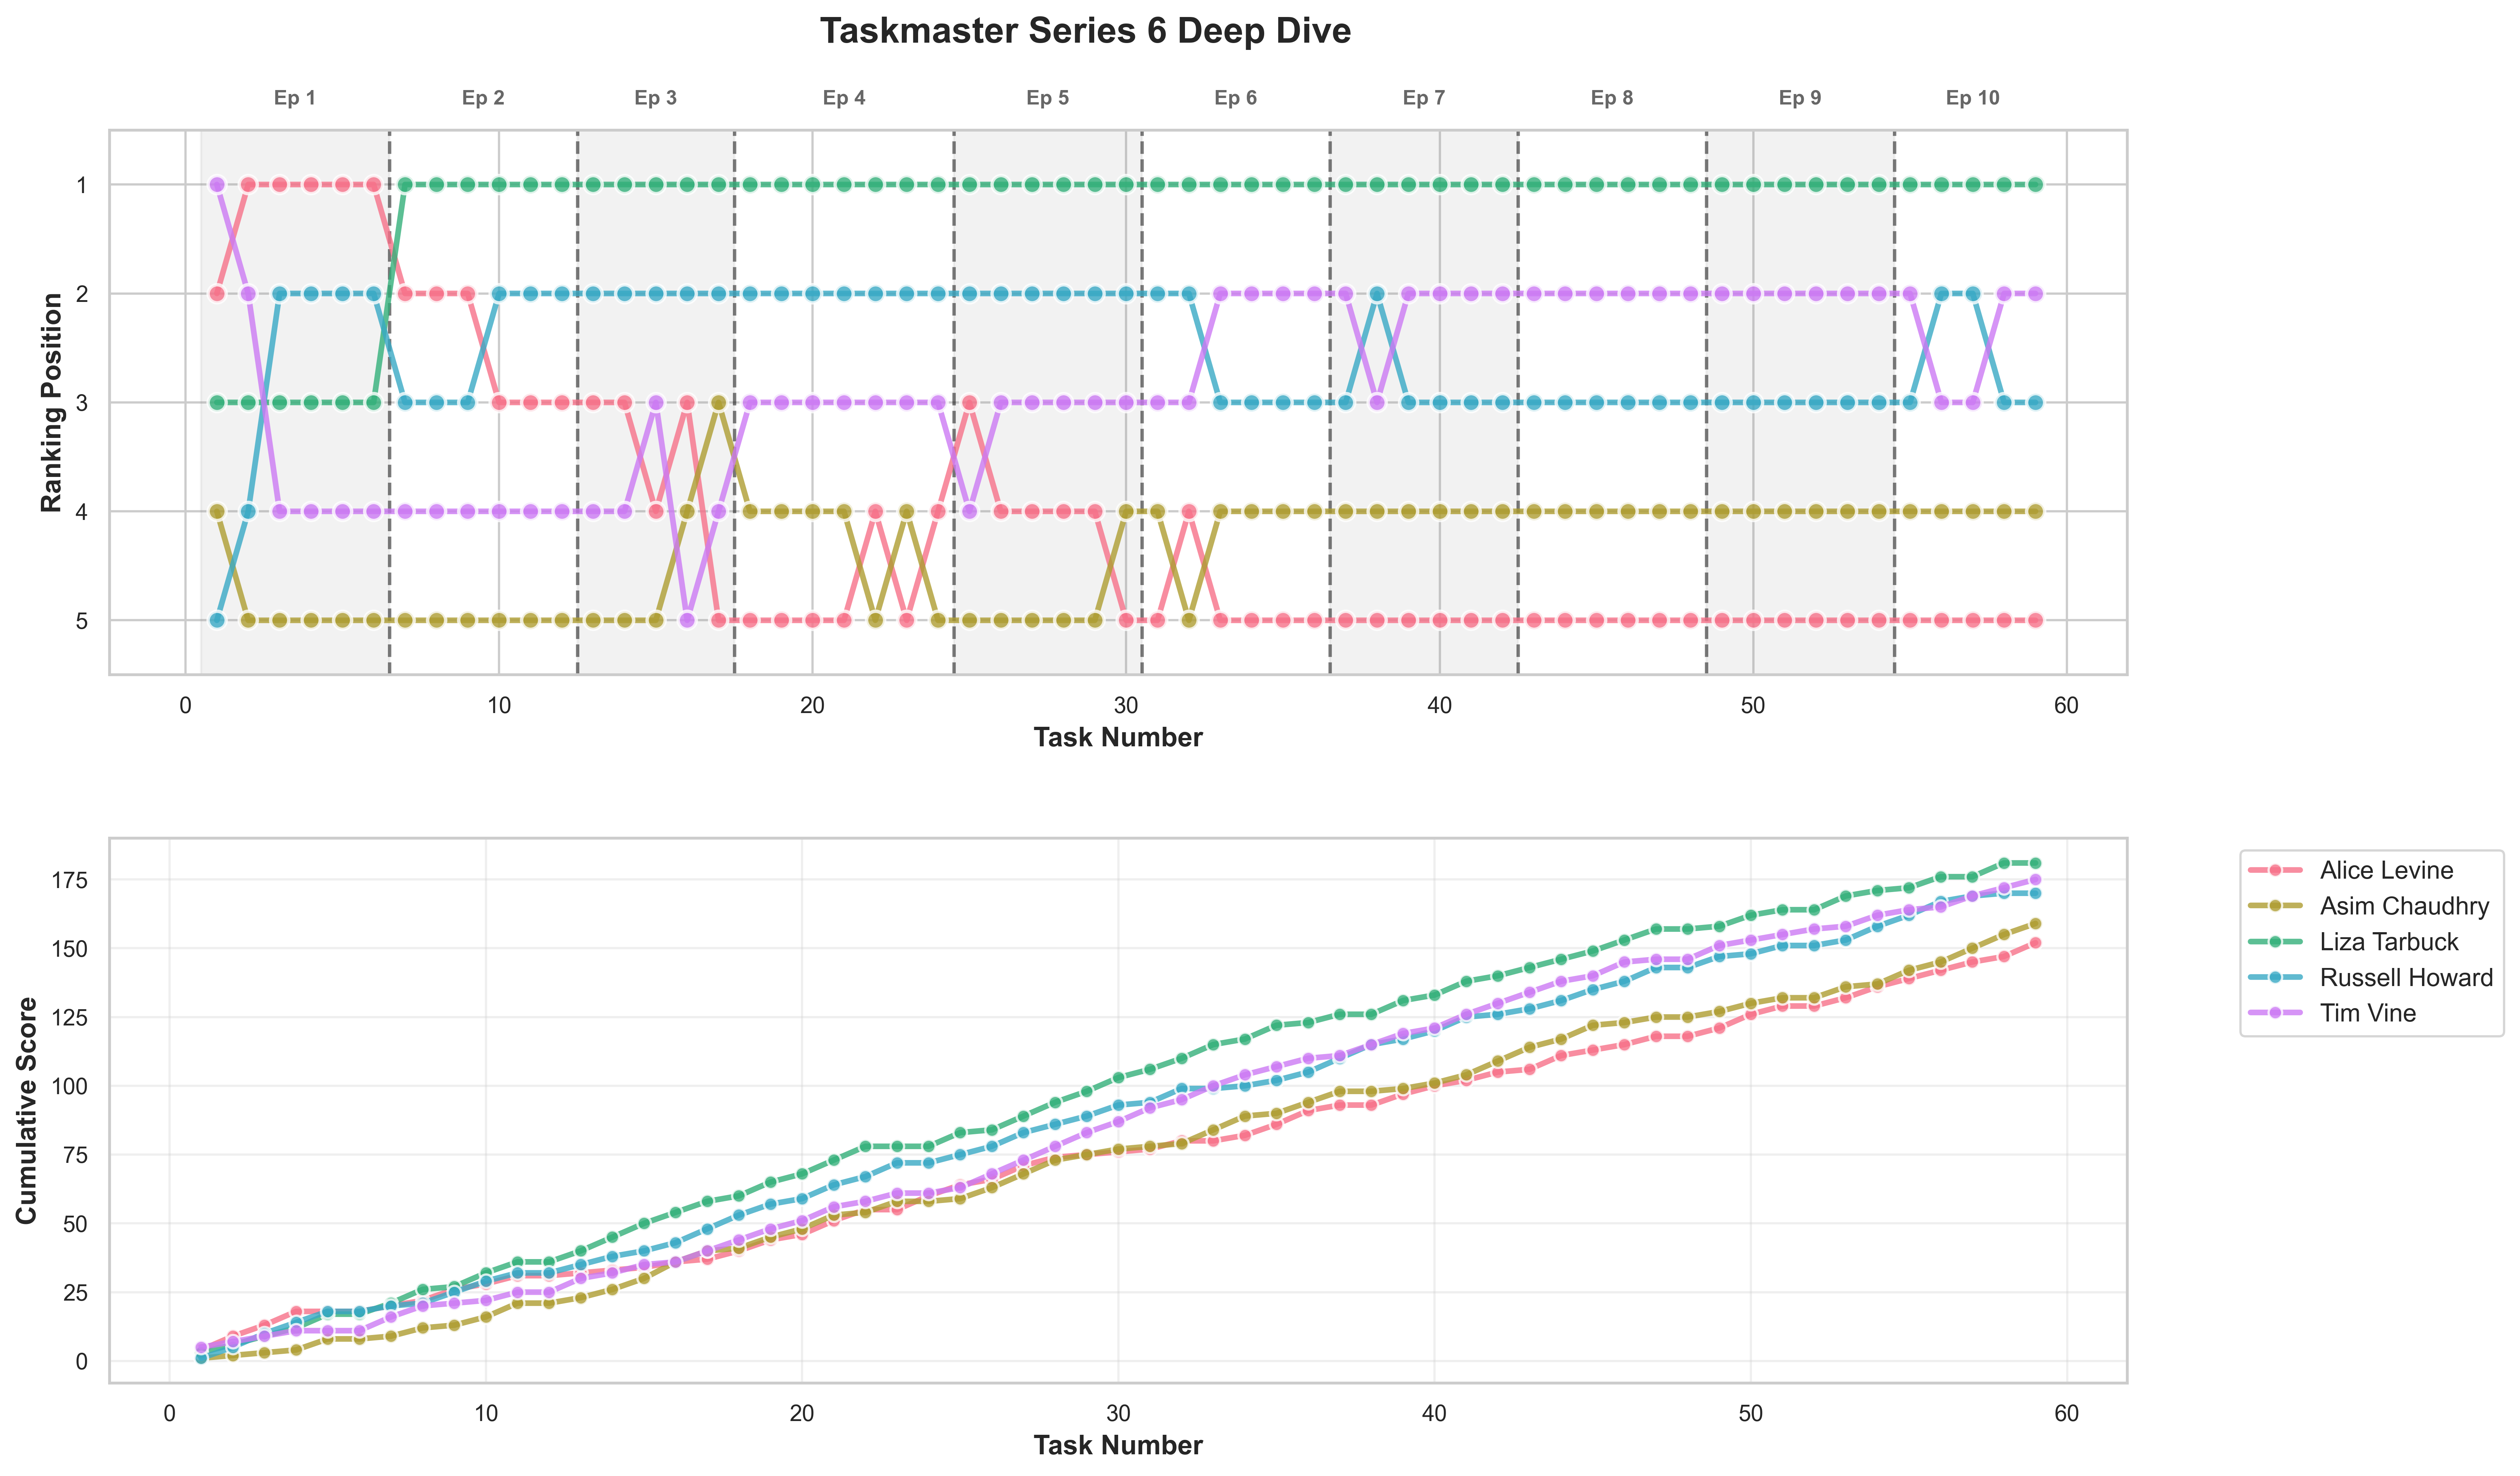
\includegraphics[width=\linewidth]{figures/supplementary/series_6_deep_dive.png}
\end{figure}
\FloatBarrier
\clearpage

\begin{figure}[!h]
\centering
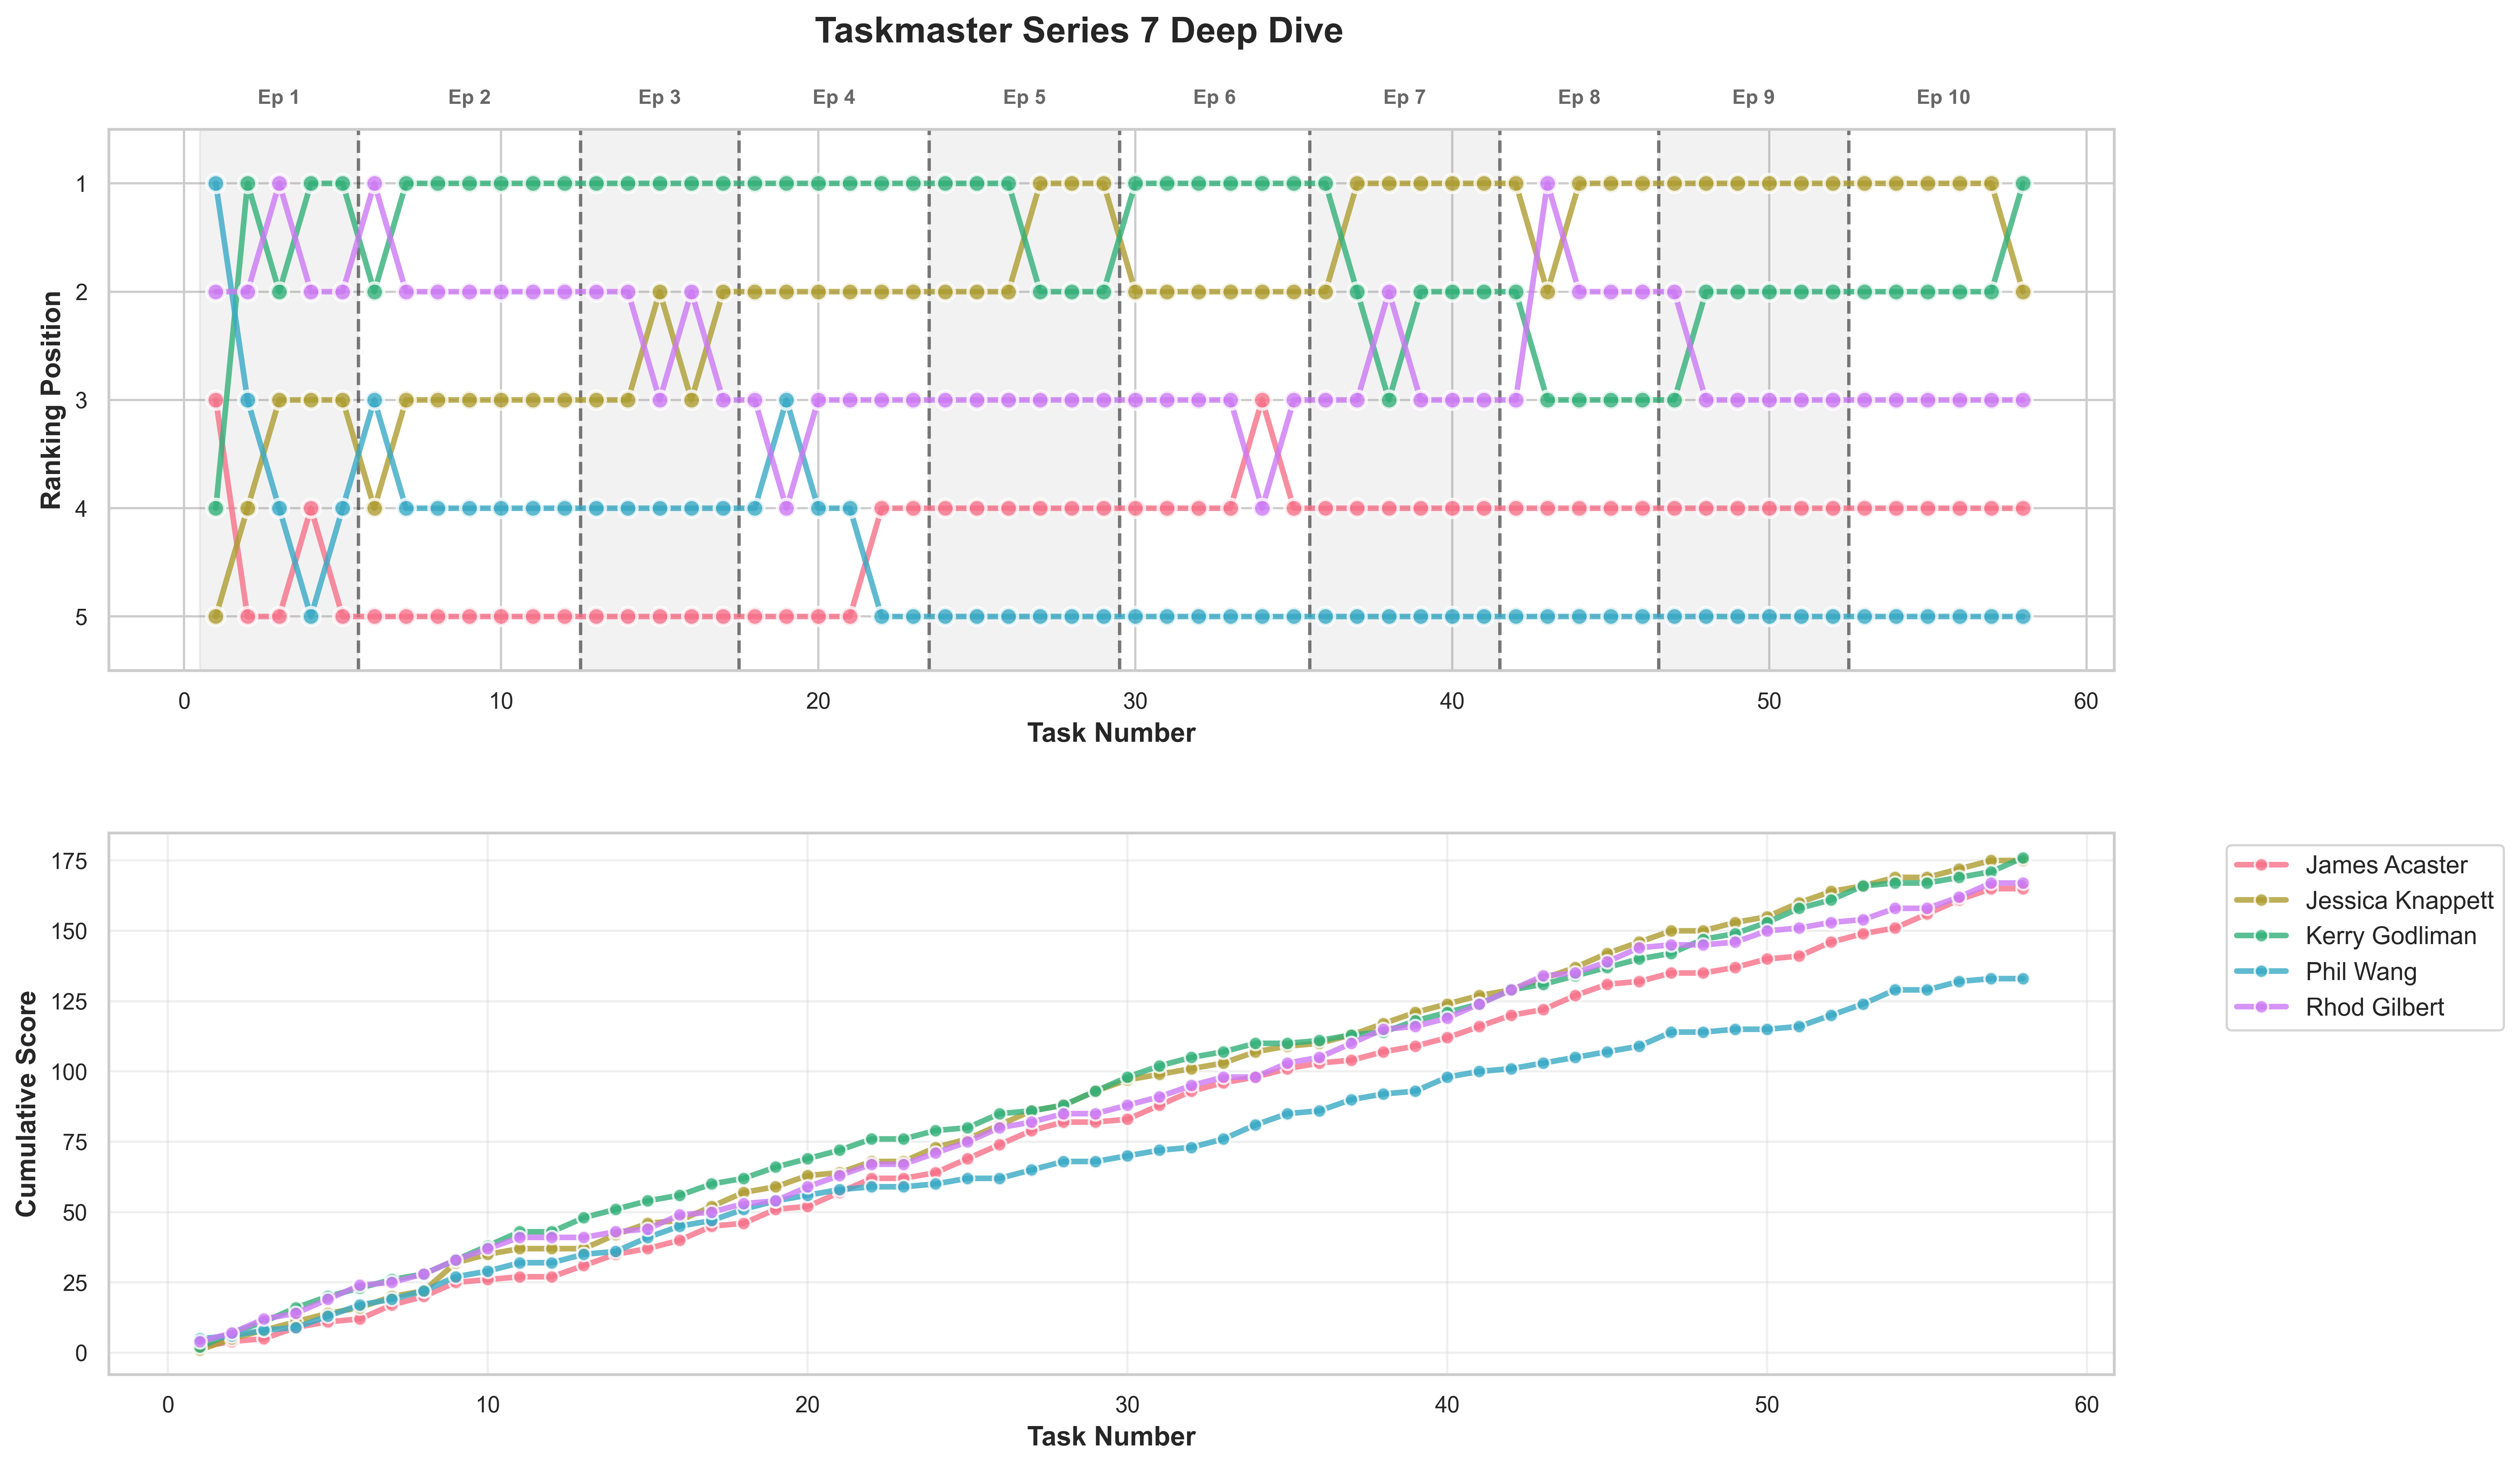
\includegraphics[width=\linewidth]{figures/supplementary/series_7_deep_dive.png}
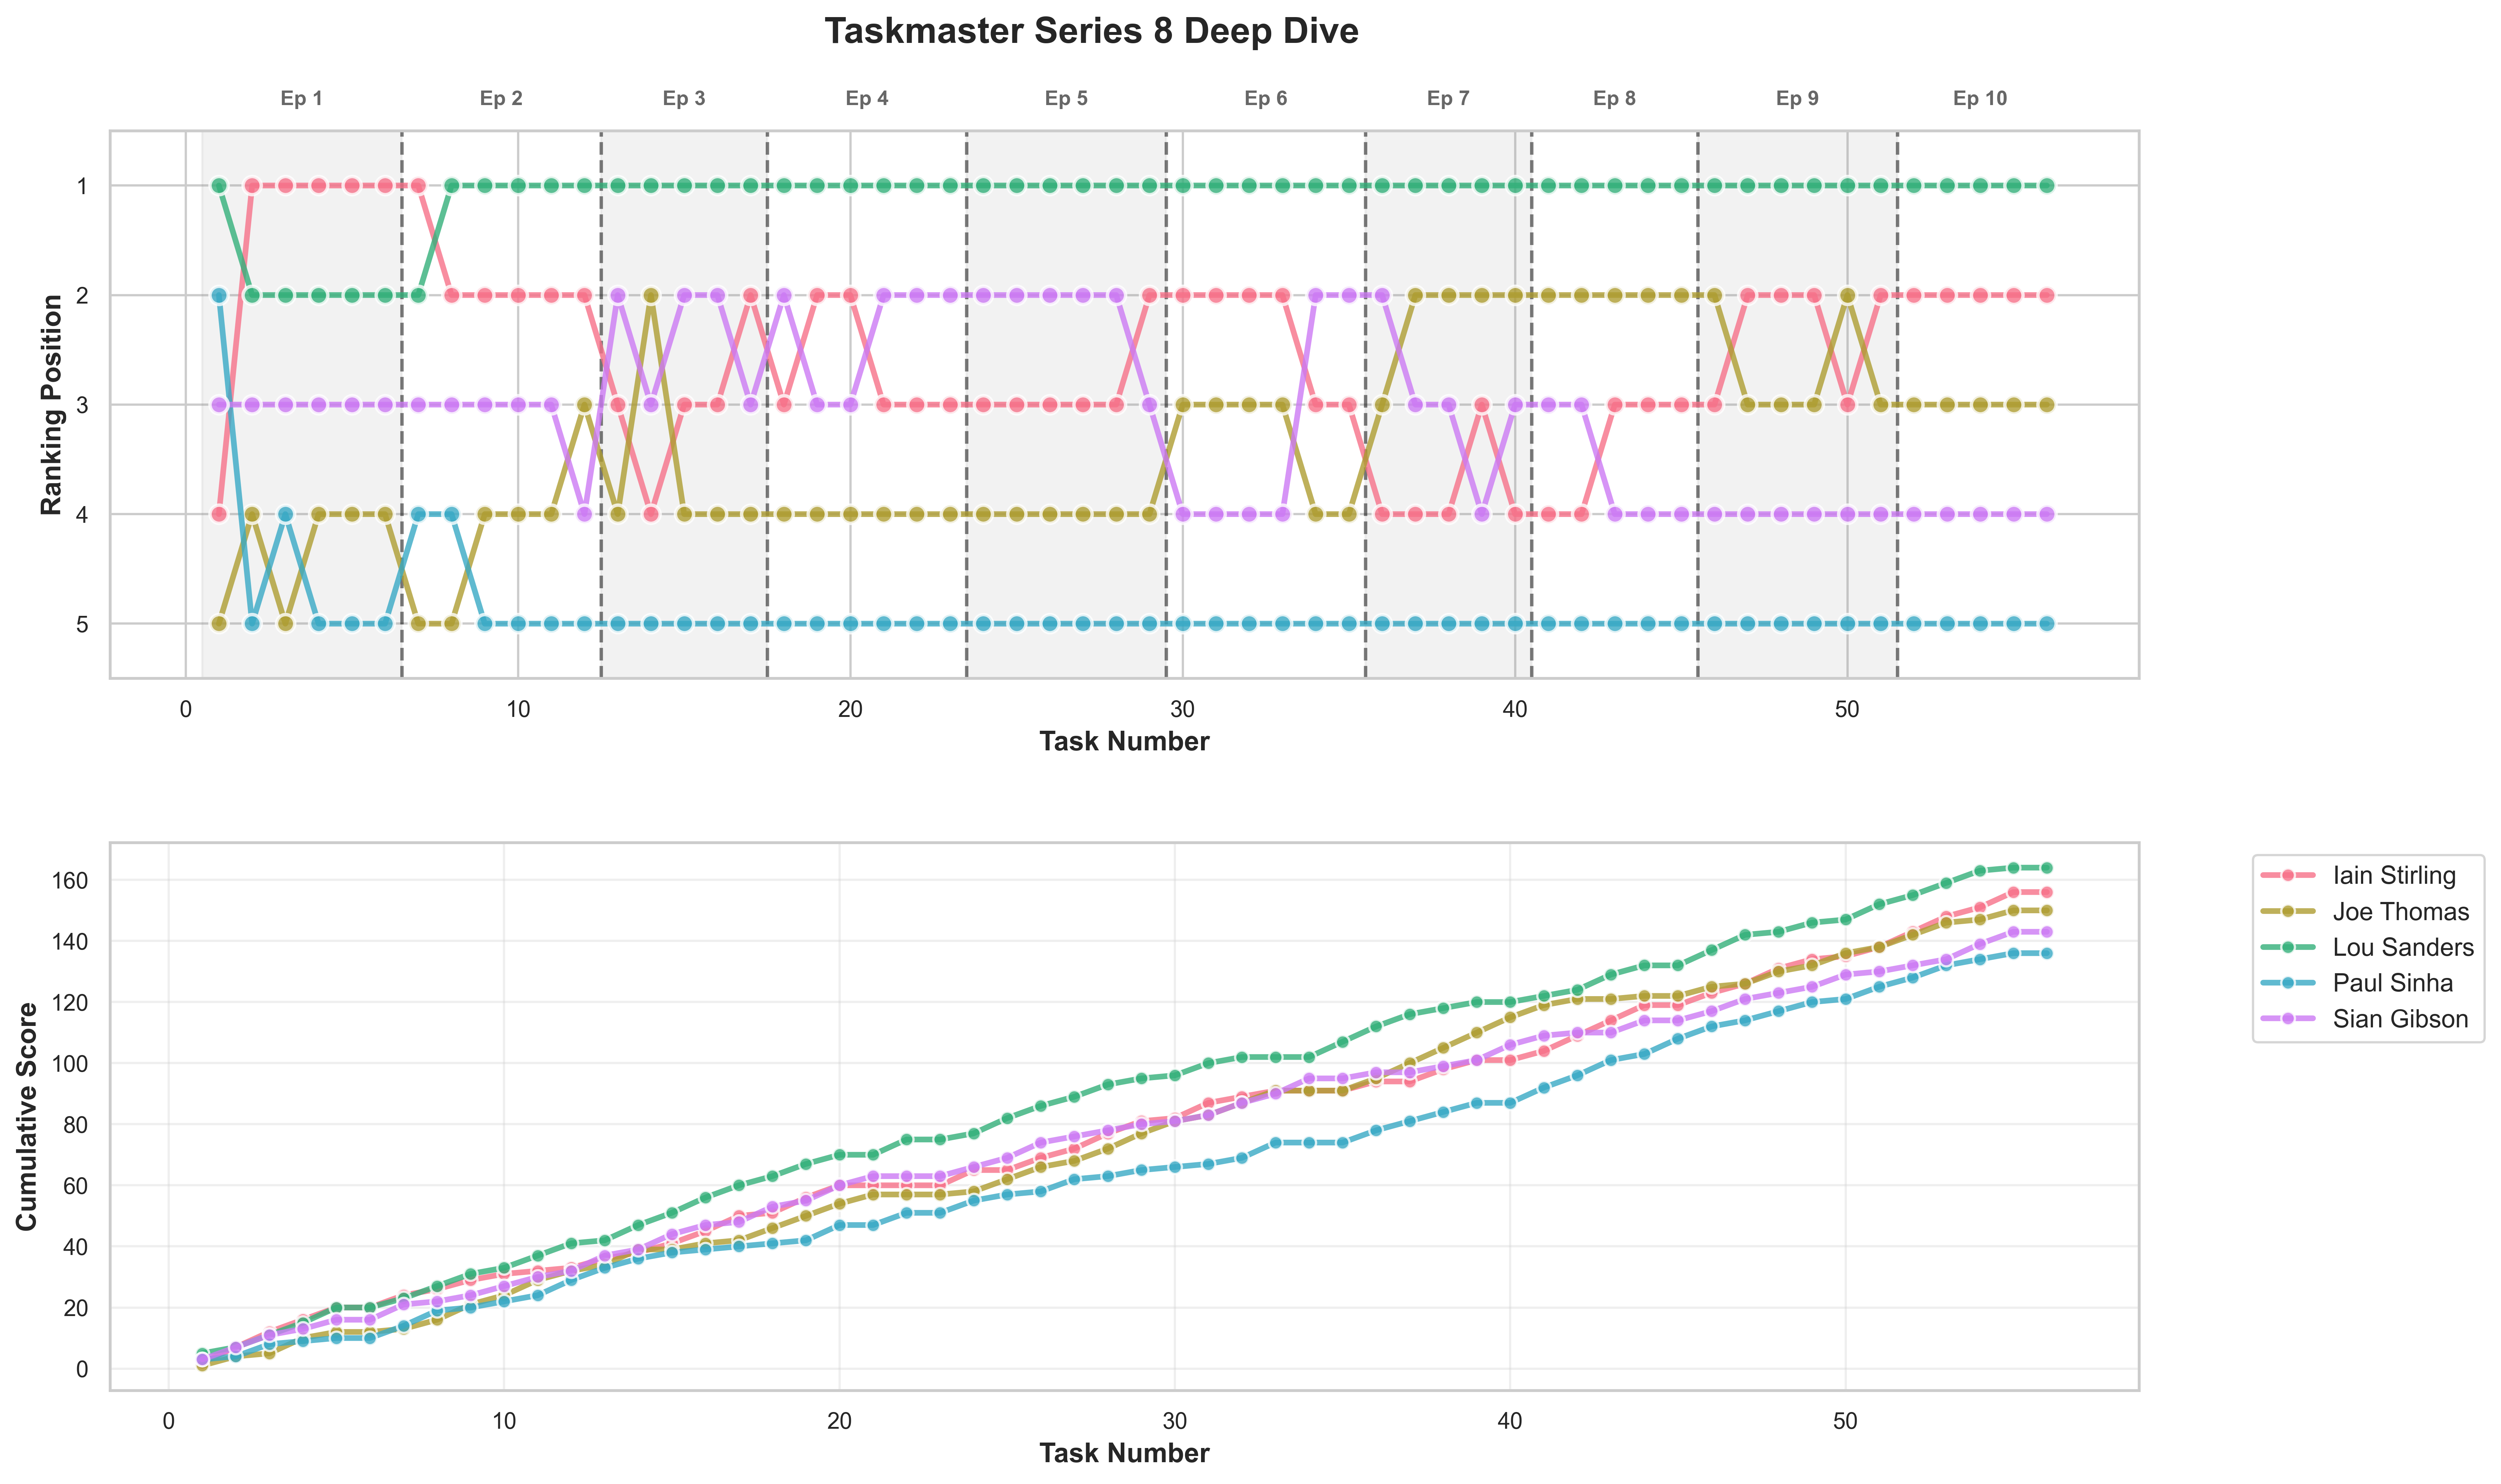
\includegraphics[width=\linewidth]{figures/supplementary/series_8_deep_dive.png}
\end{figure}
\FloatBarrier
\clearpage

\begin{figure}[!h]
\centering
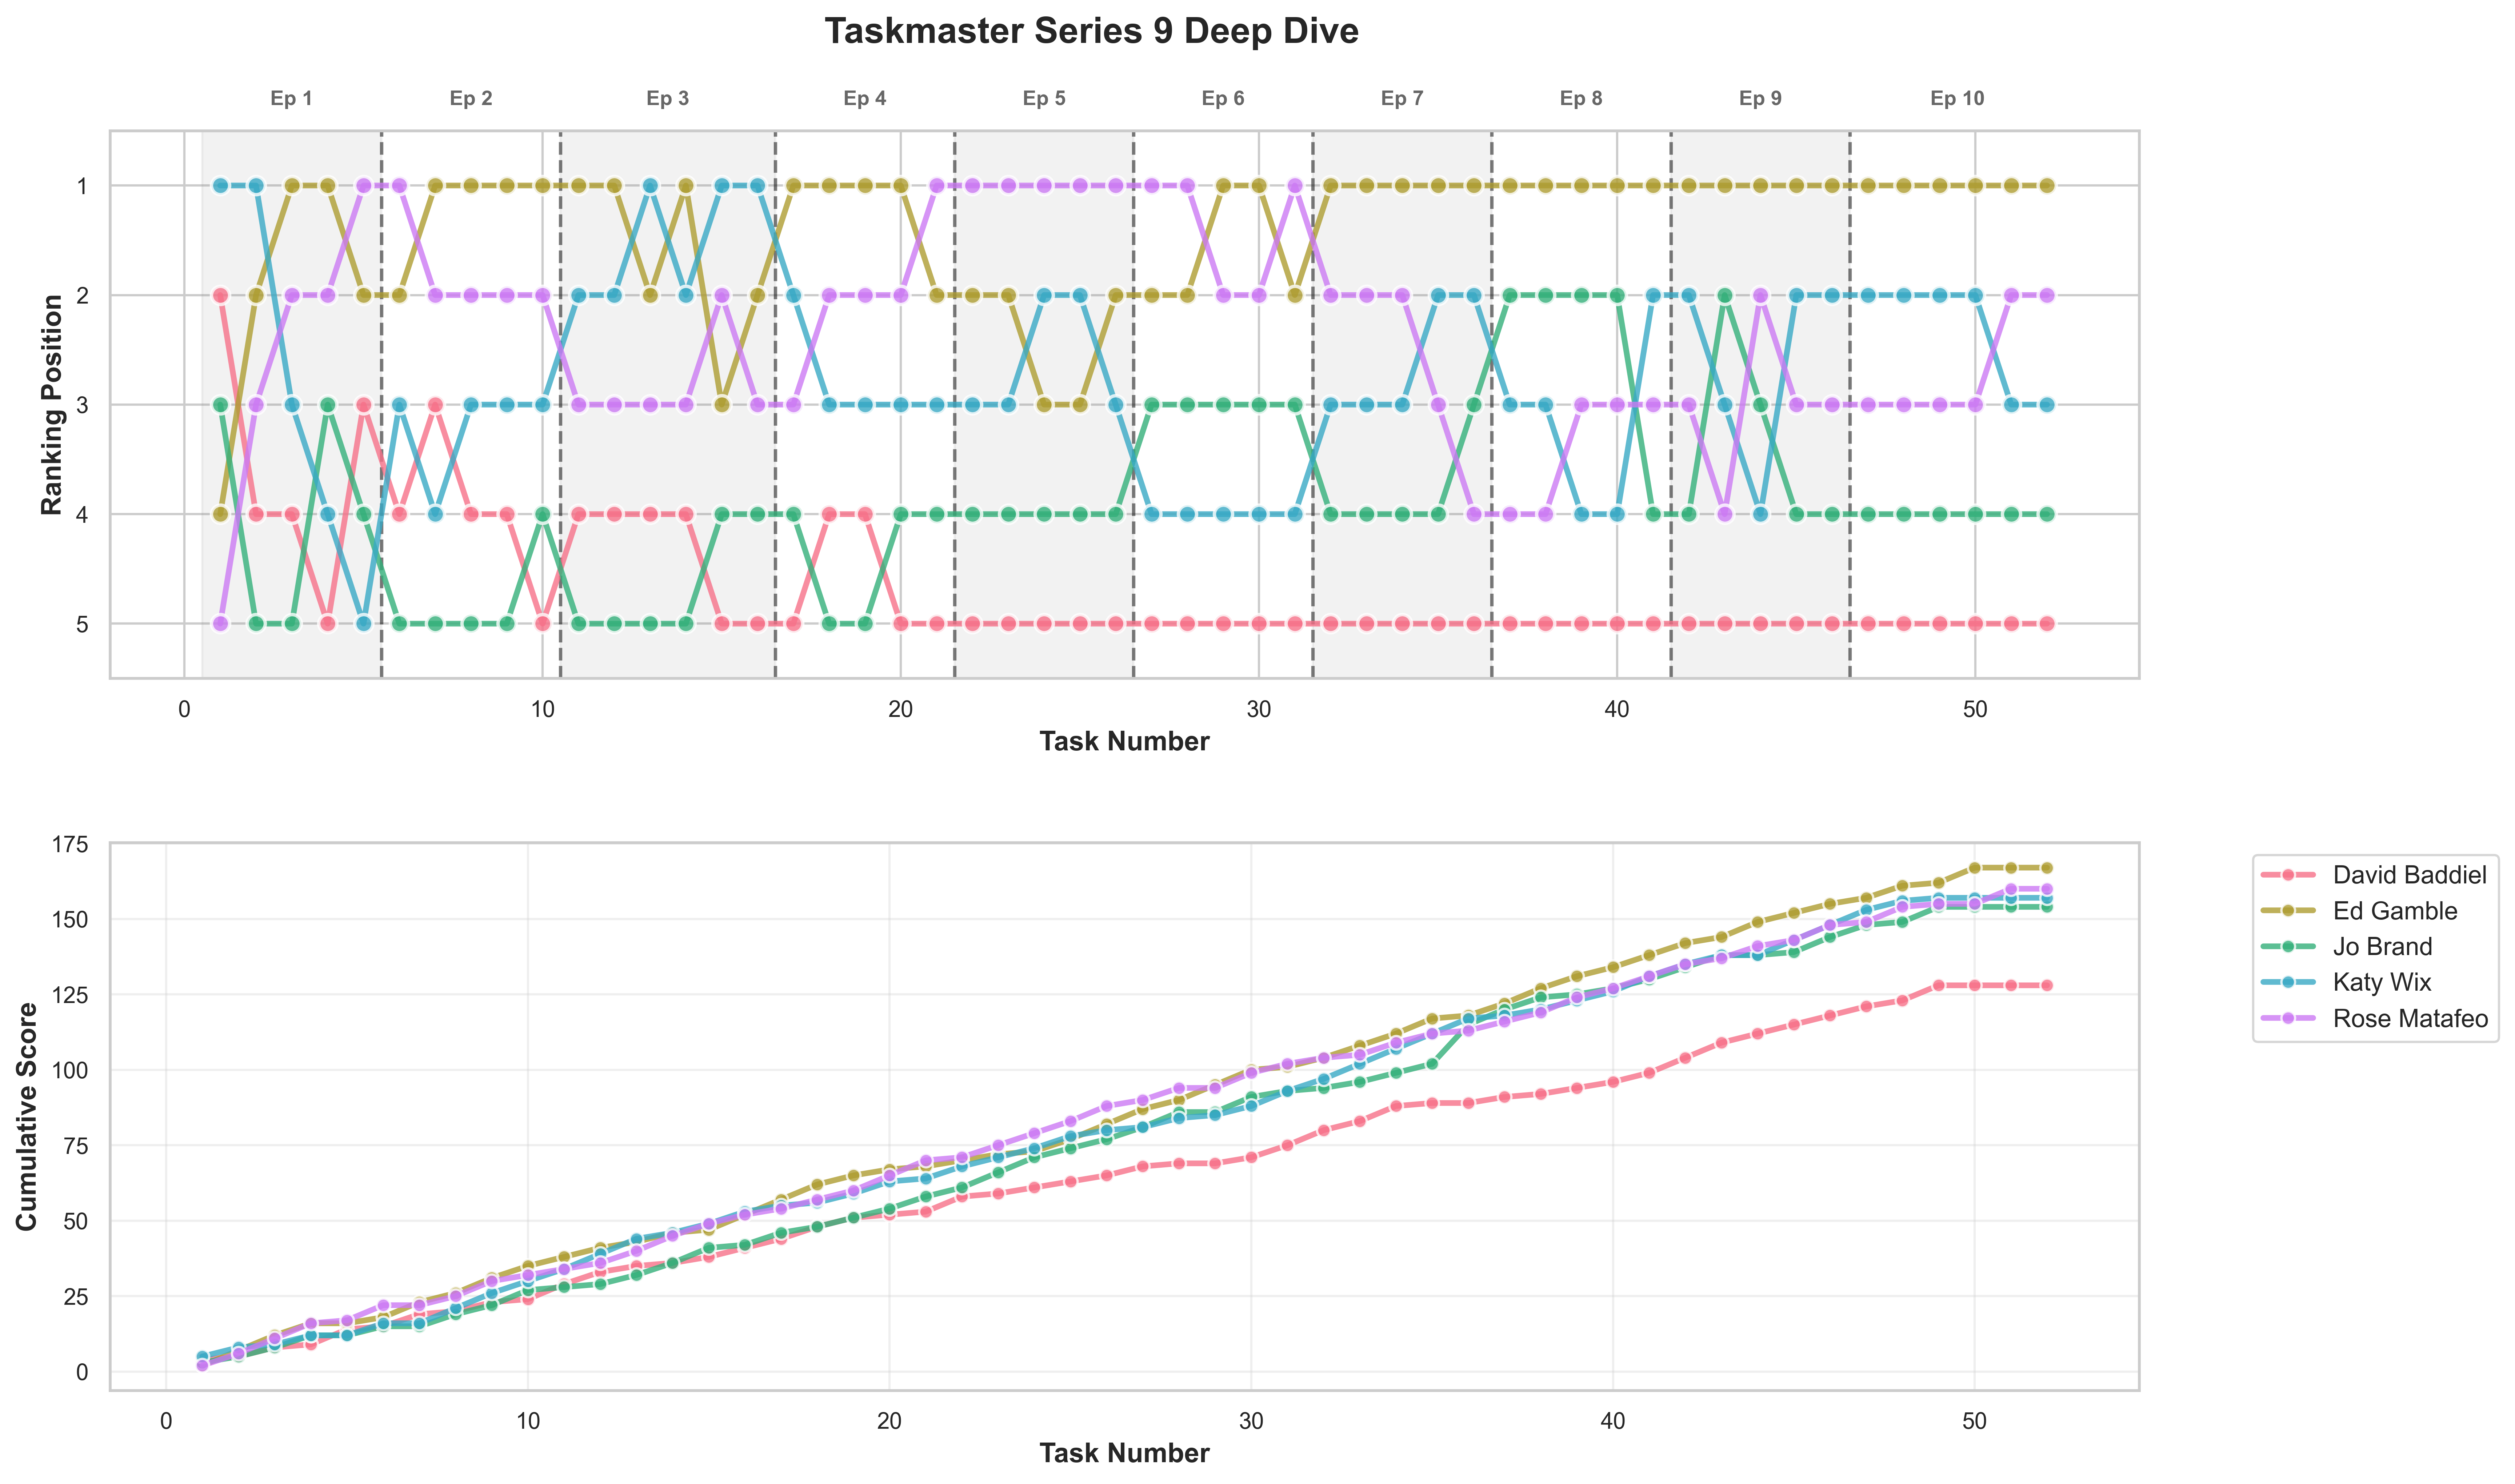
\includegraphics[width=\linewidth]{figures/supplementary/series_9_deep_dive.png}
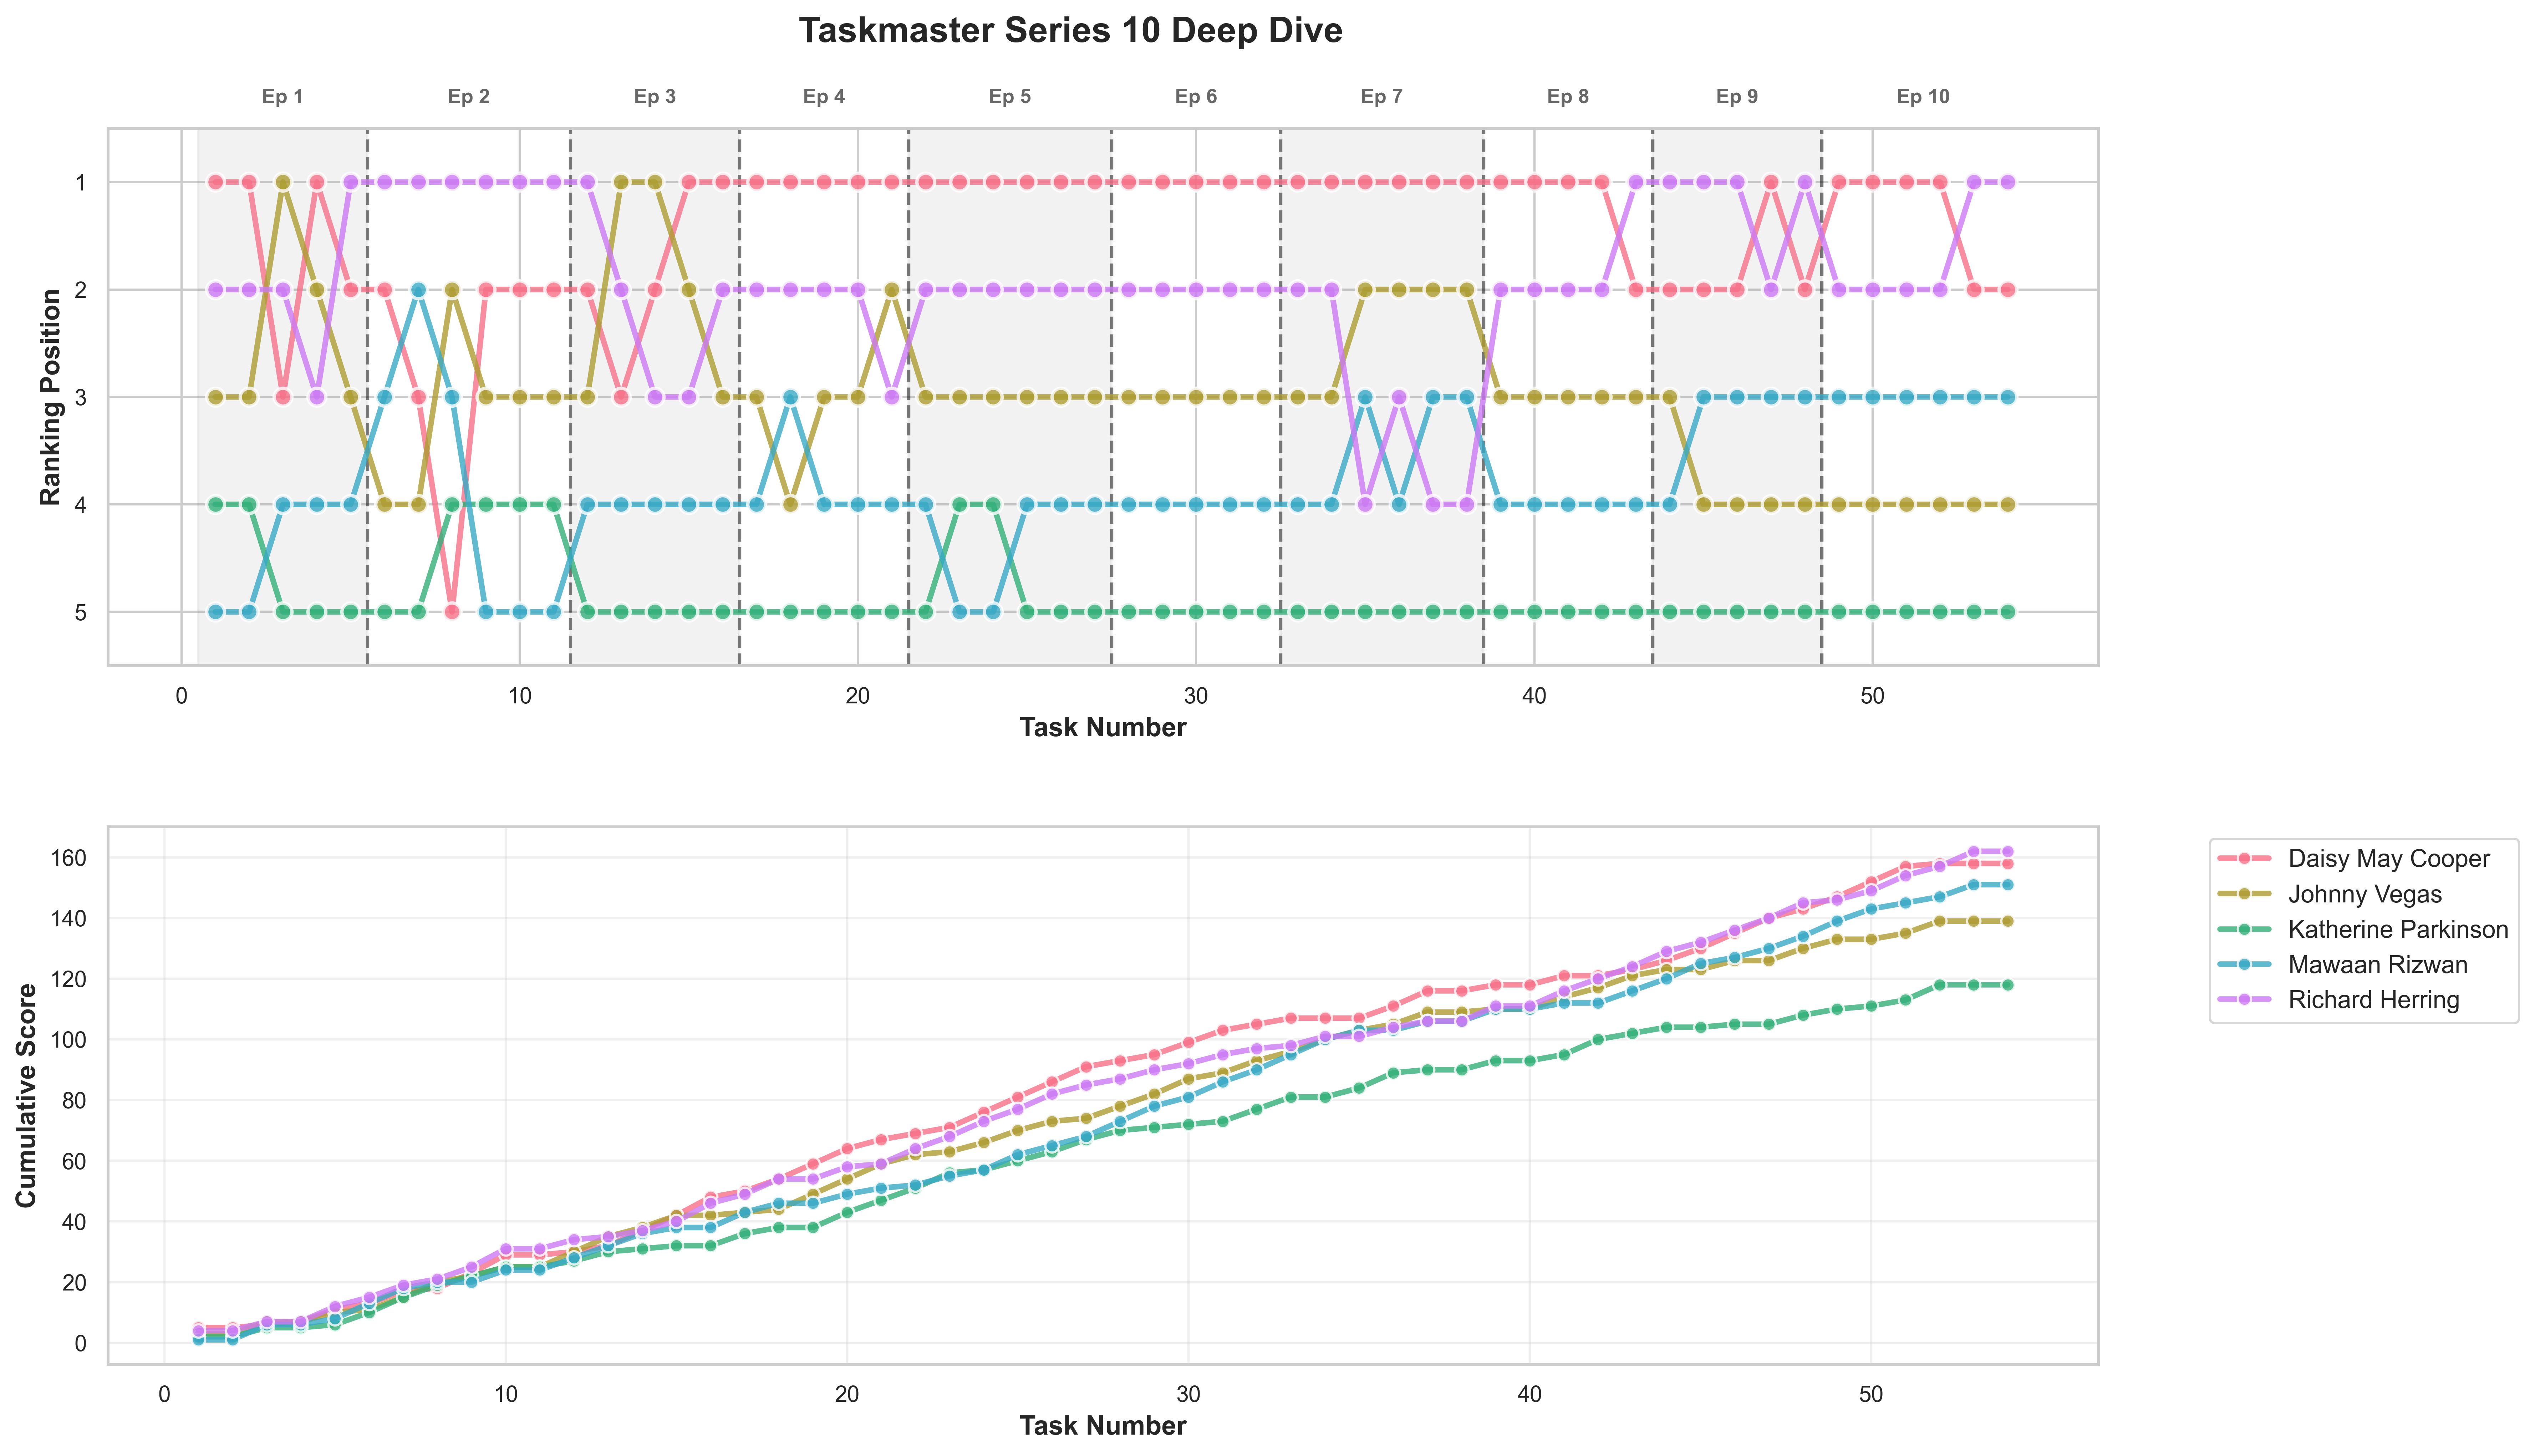
\includegraphics[width=\linewidth]{figures/supplementary/series_10_deep_dive.png}
\end{figure}
\FloatBarrier
\clearpage

\begin{figure}[!h]
\centering
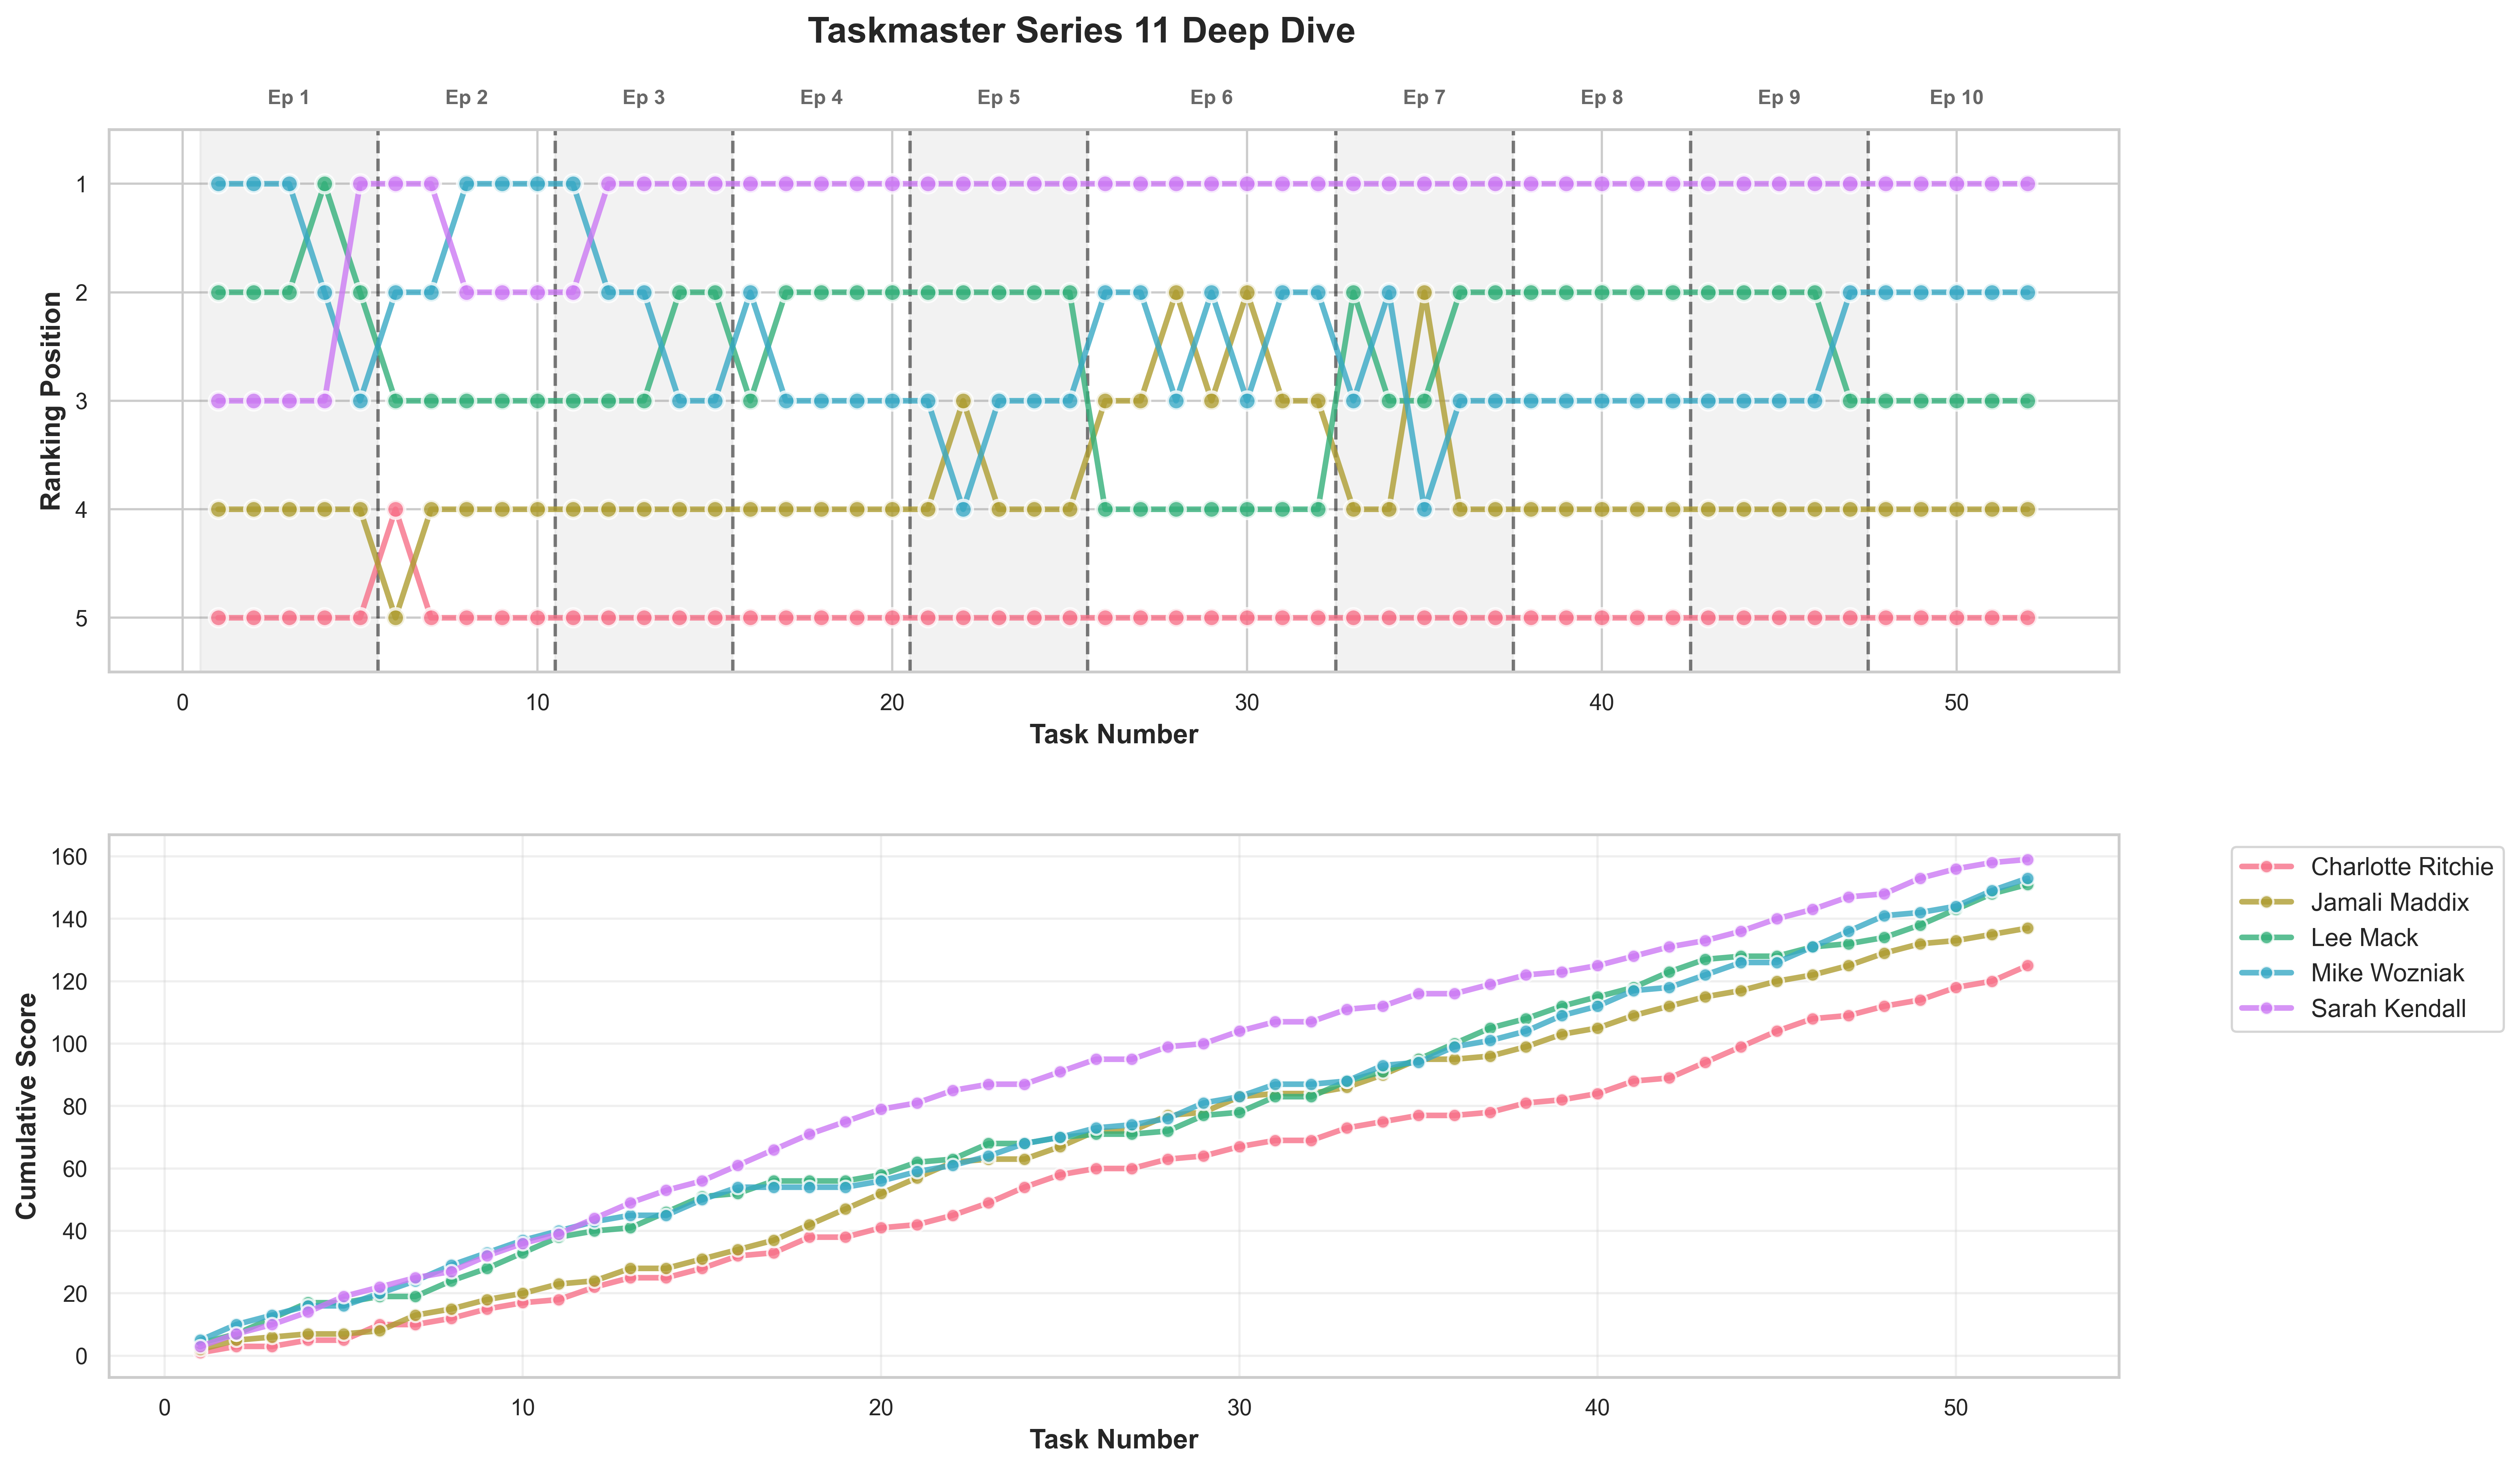
\includegraphics[width=\linewidth]{figures/supplementary/series_11_deep_dive.png}
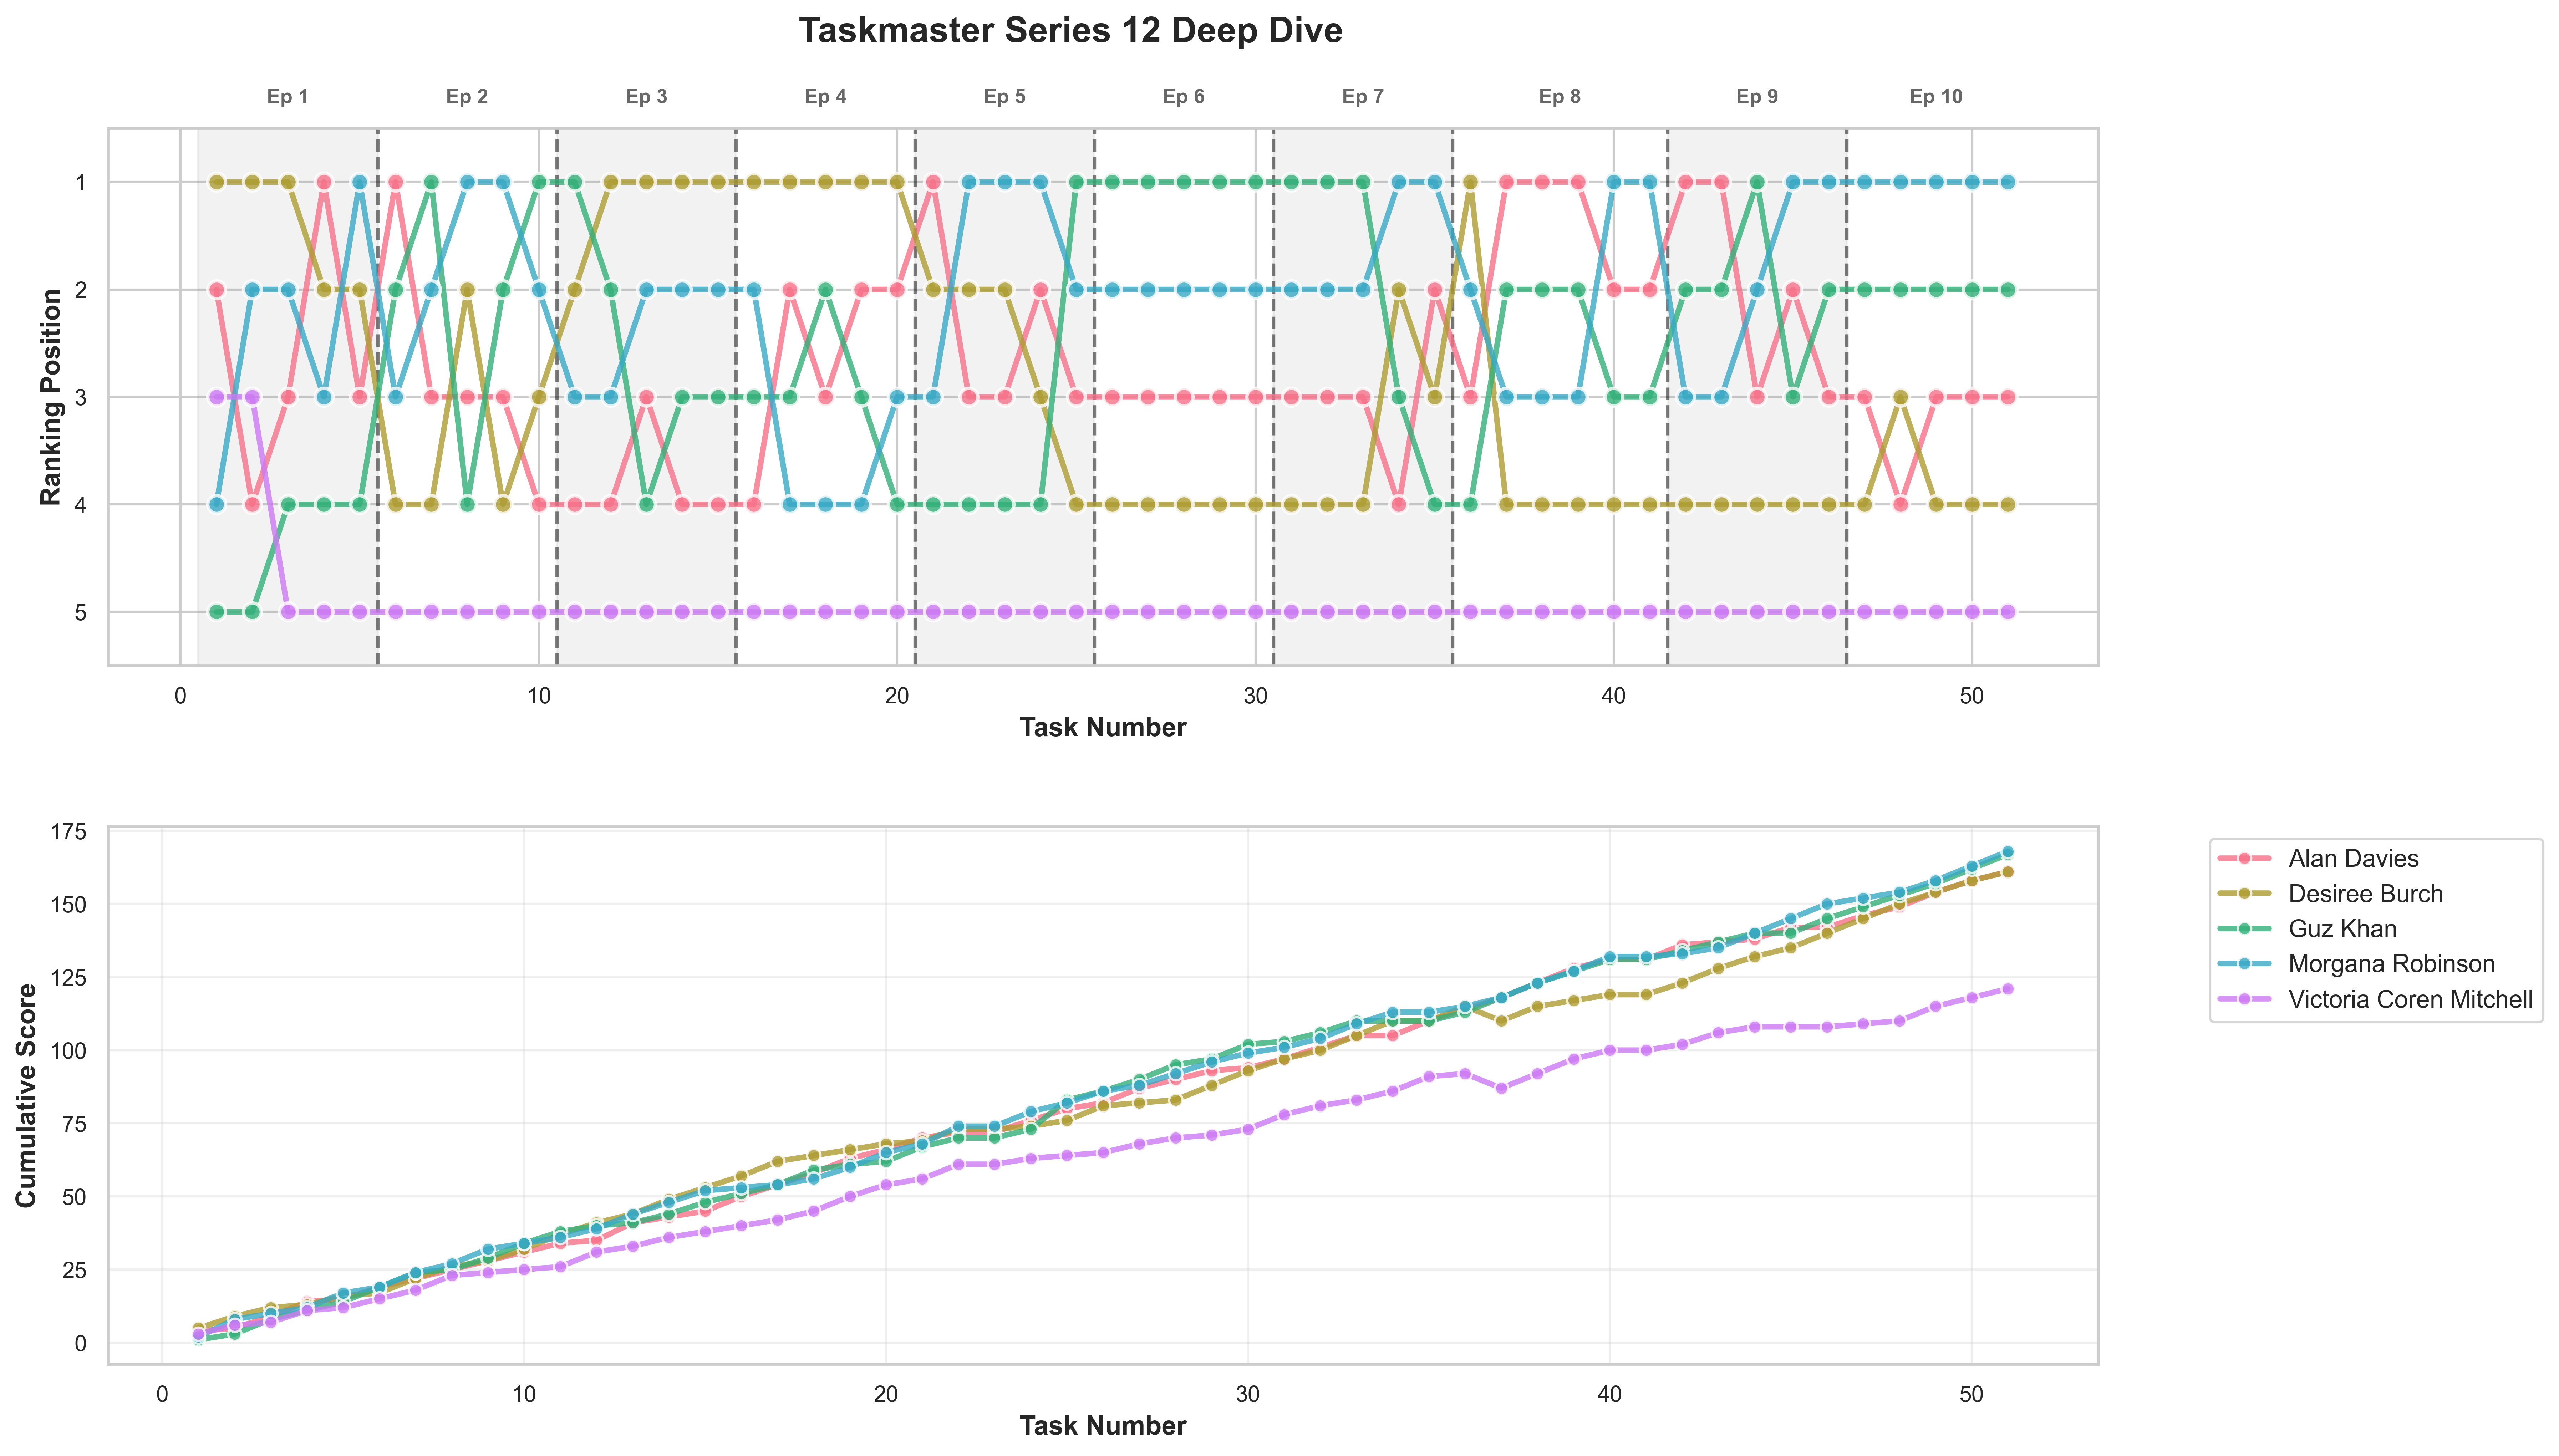
\includegraphics[width=\linewidth]{figures/supplementary/series_12_deep_dive.png}
\end{figure}
\FloatBarrier
\clearpage

\begin{figure}[!h]
\centering
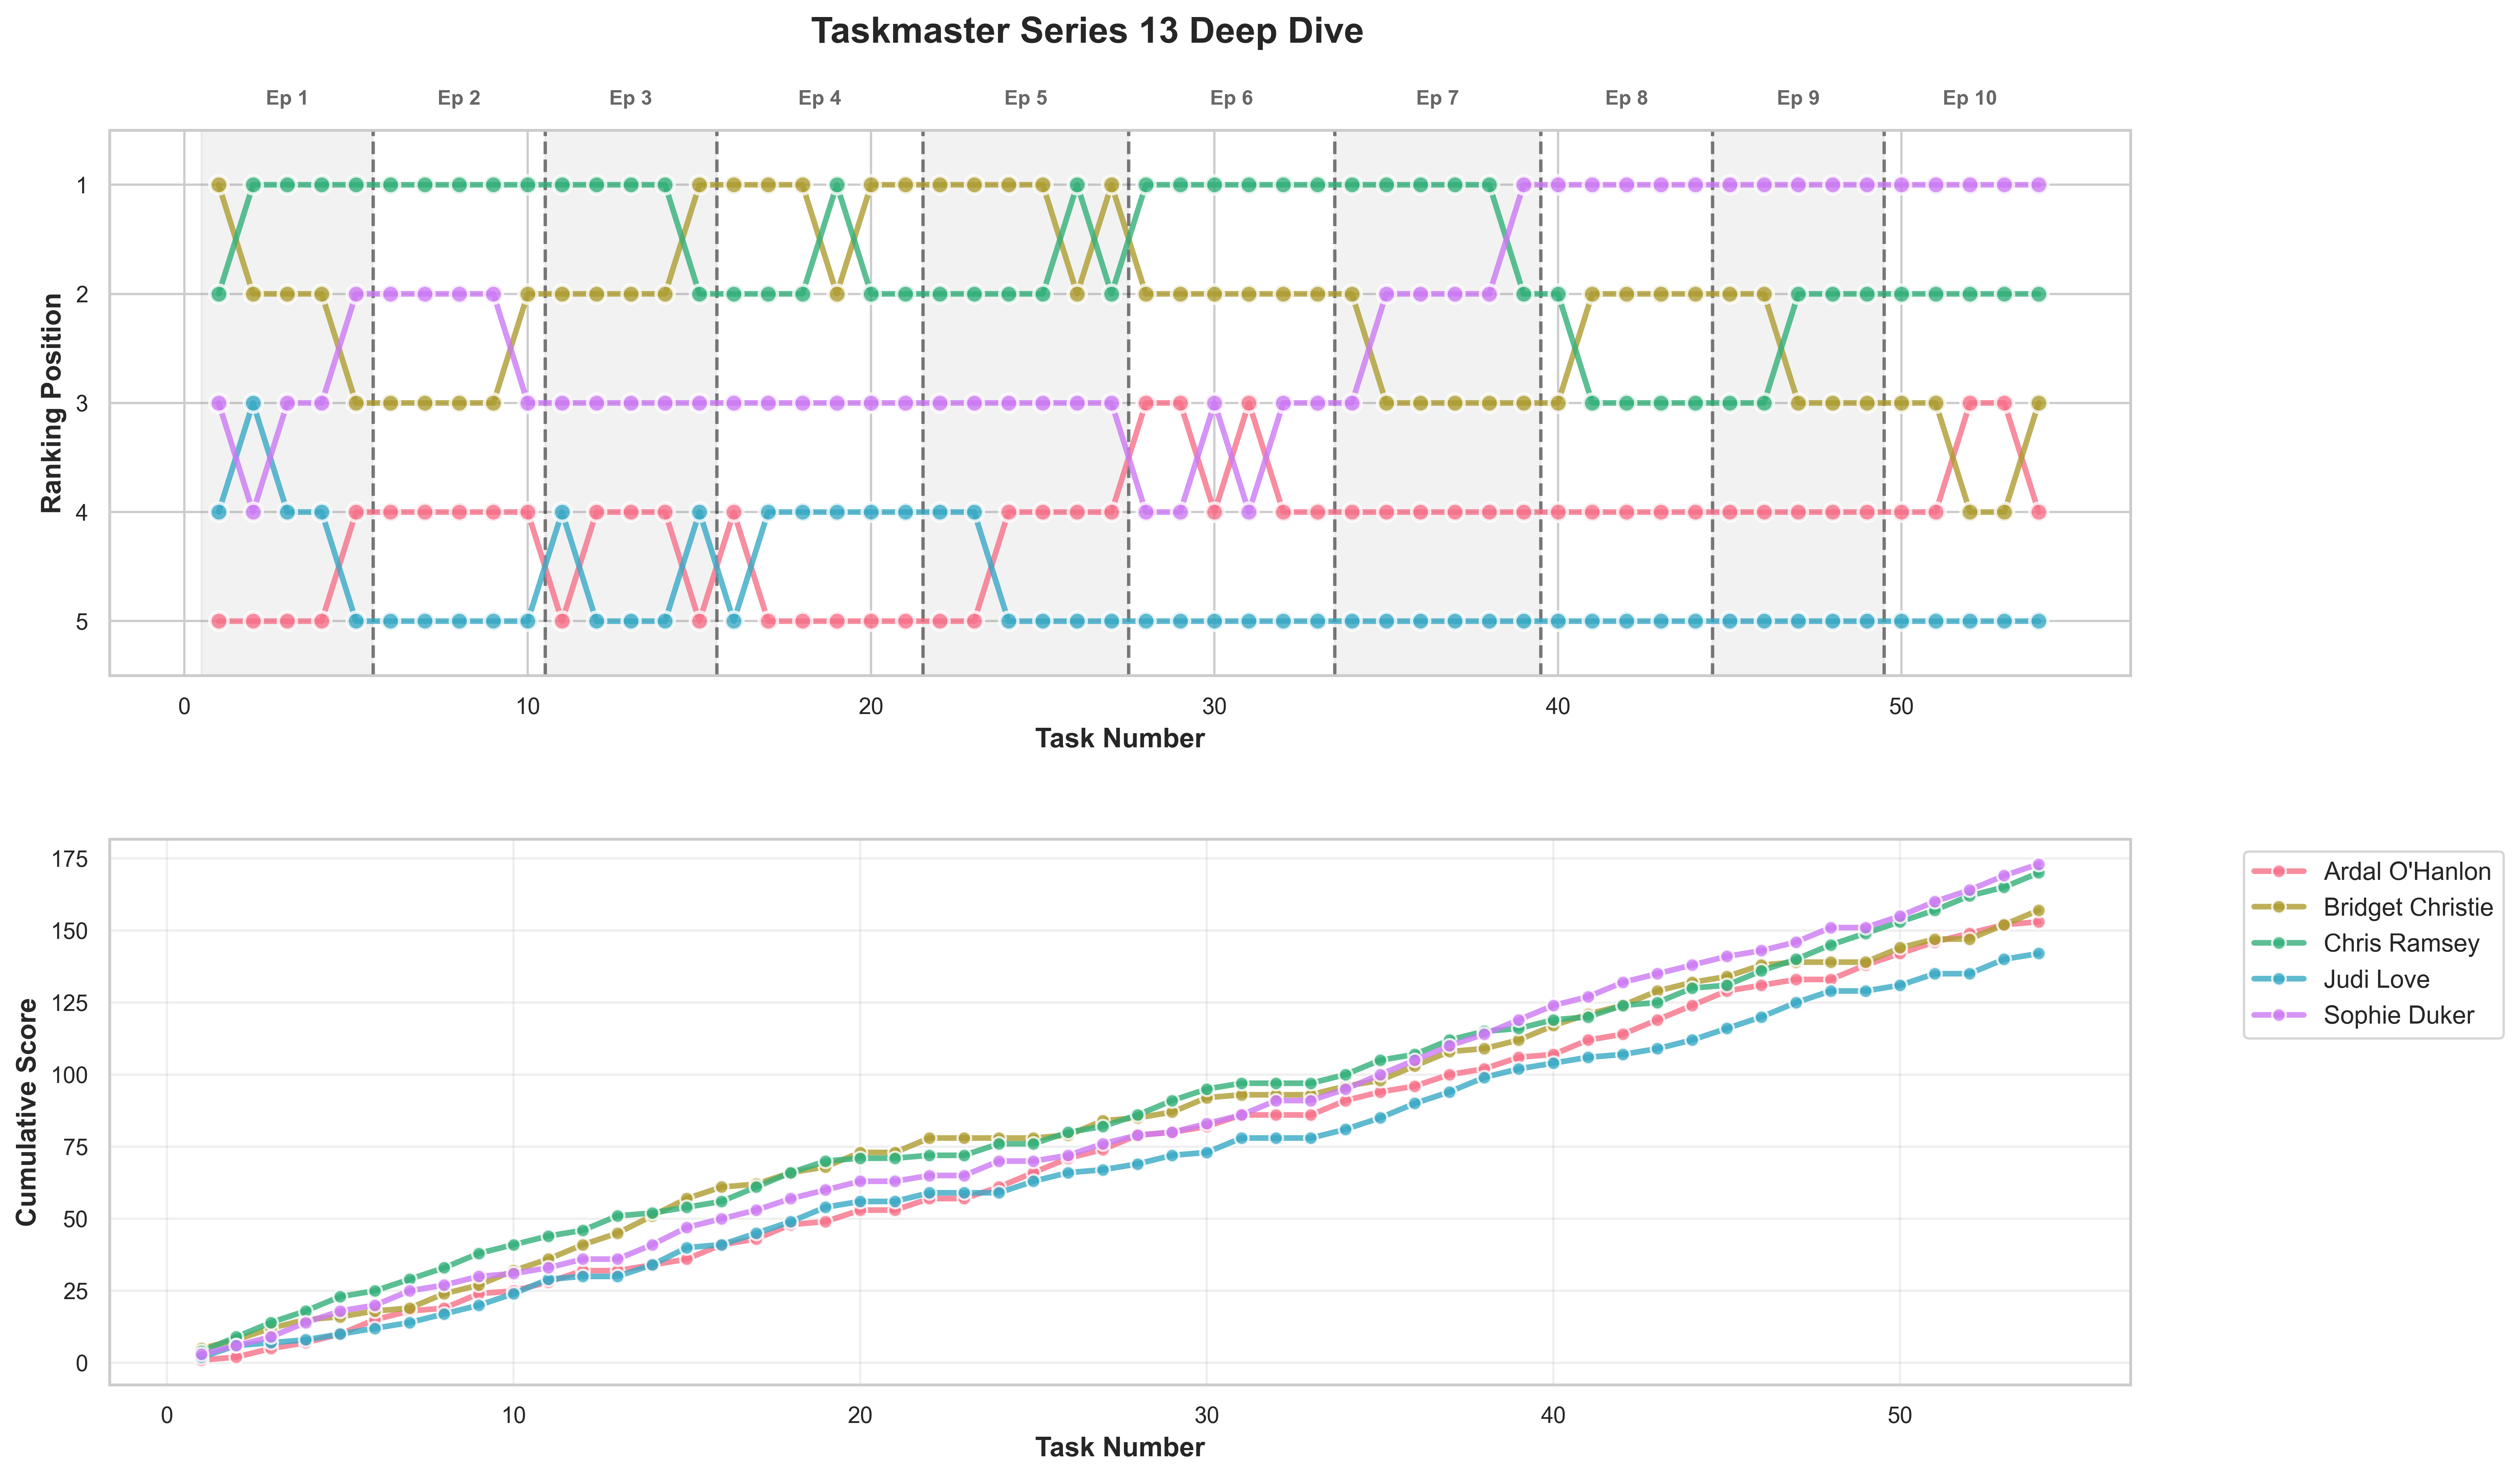
\includegraphics[width=\linewidth]{figures/supplementary/series_13_deep_dive.png}
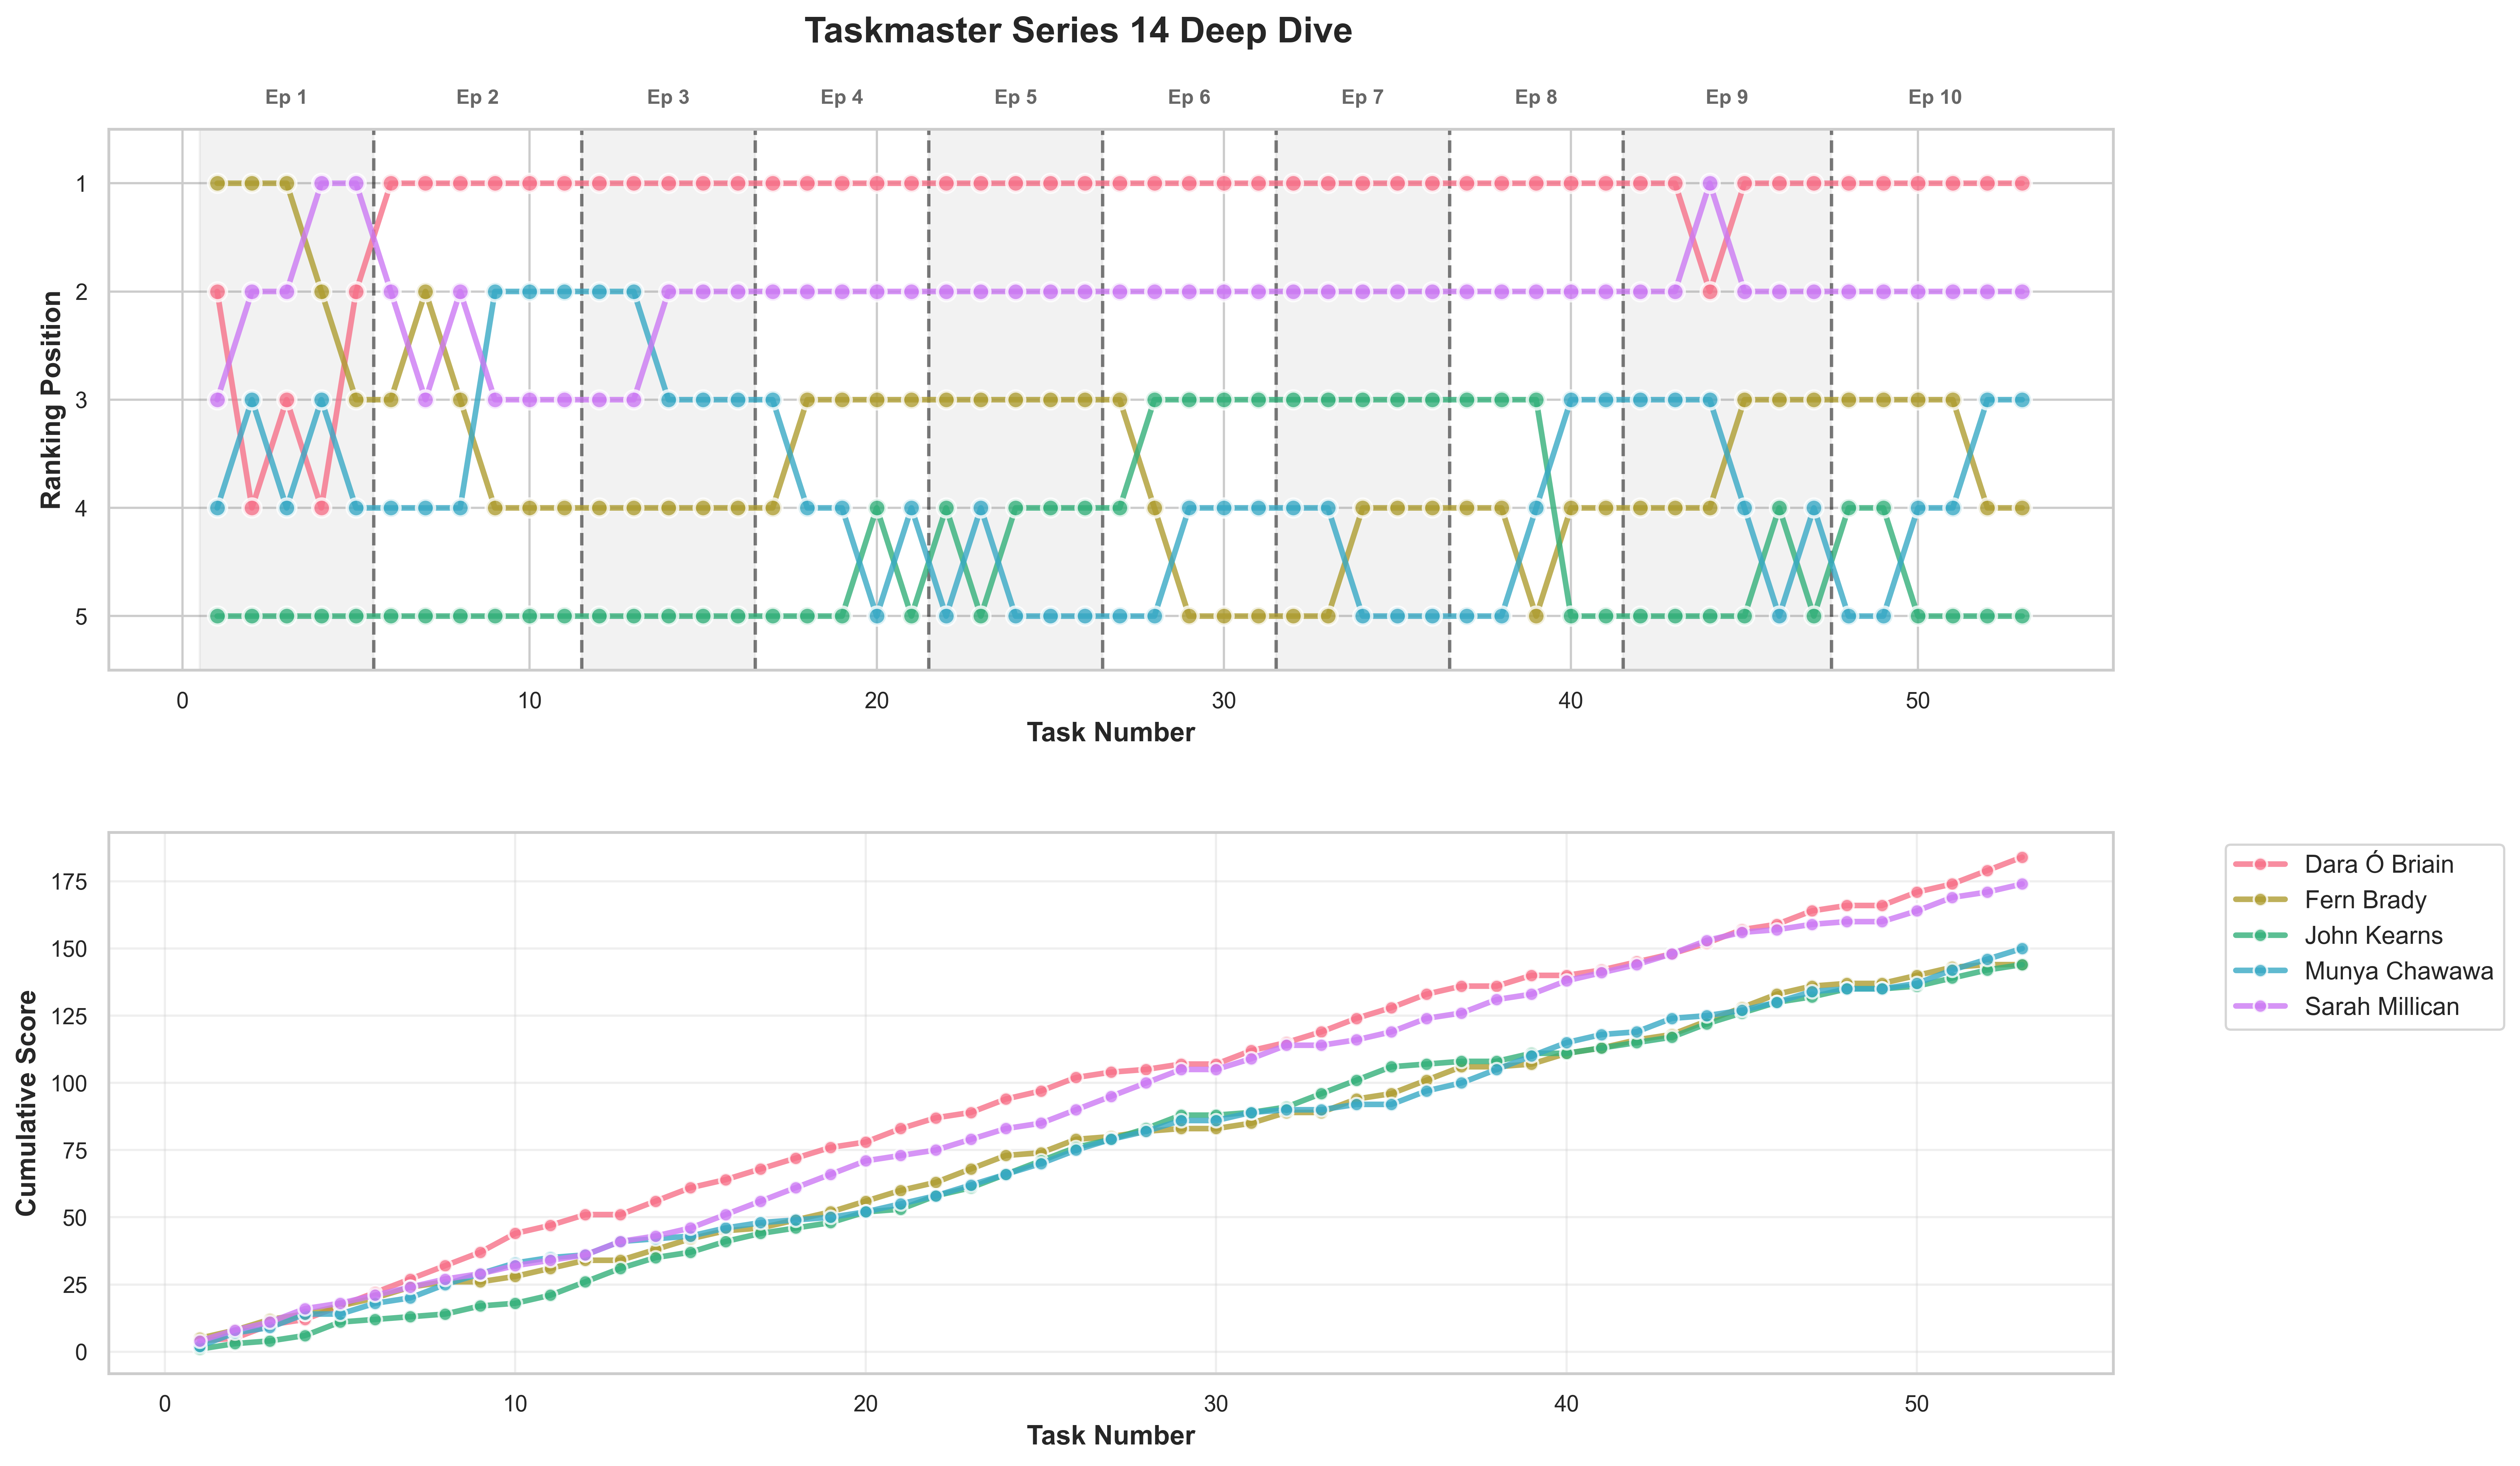
\includegraphics[width=\linewidth]{figures/supplementary/series_14_deep_dive.png}
\end{figure}
\FloatBarrier
\clearpage

\begin{figure}[!h]
\centering
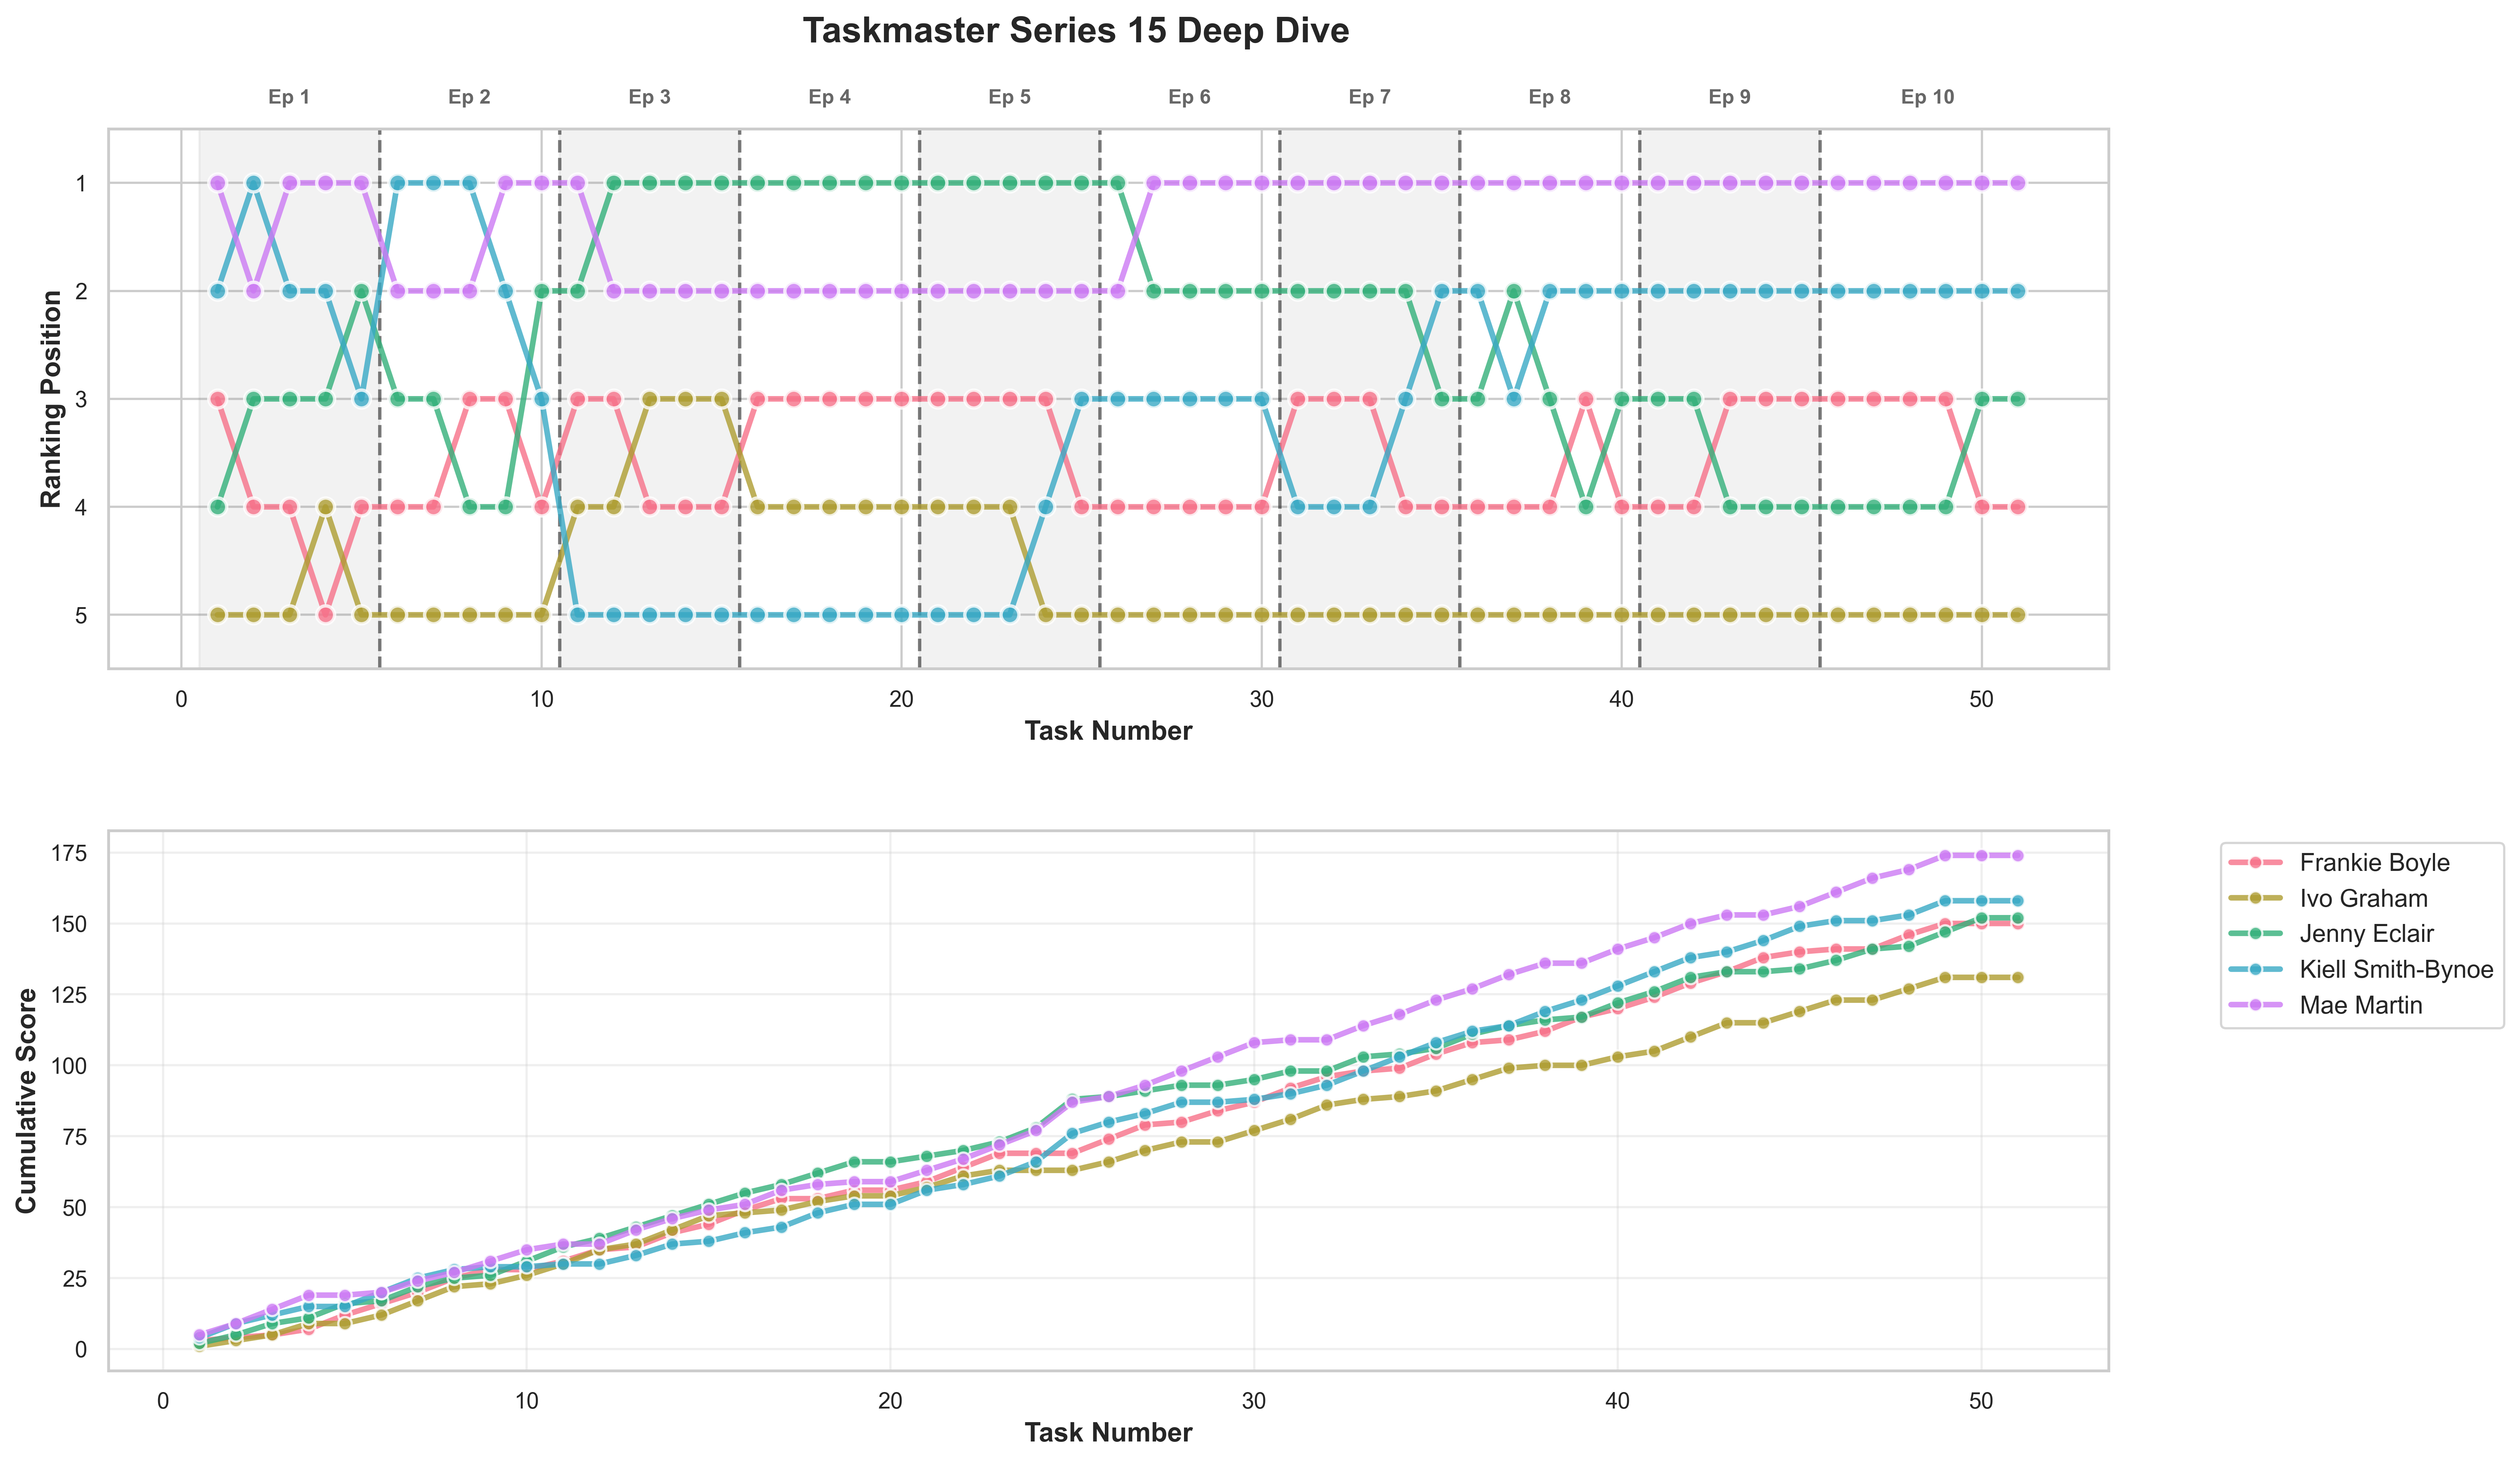
\includegraphics[width=\linewidth]{figures/supplementary/series_15_deep_dive.png}
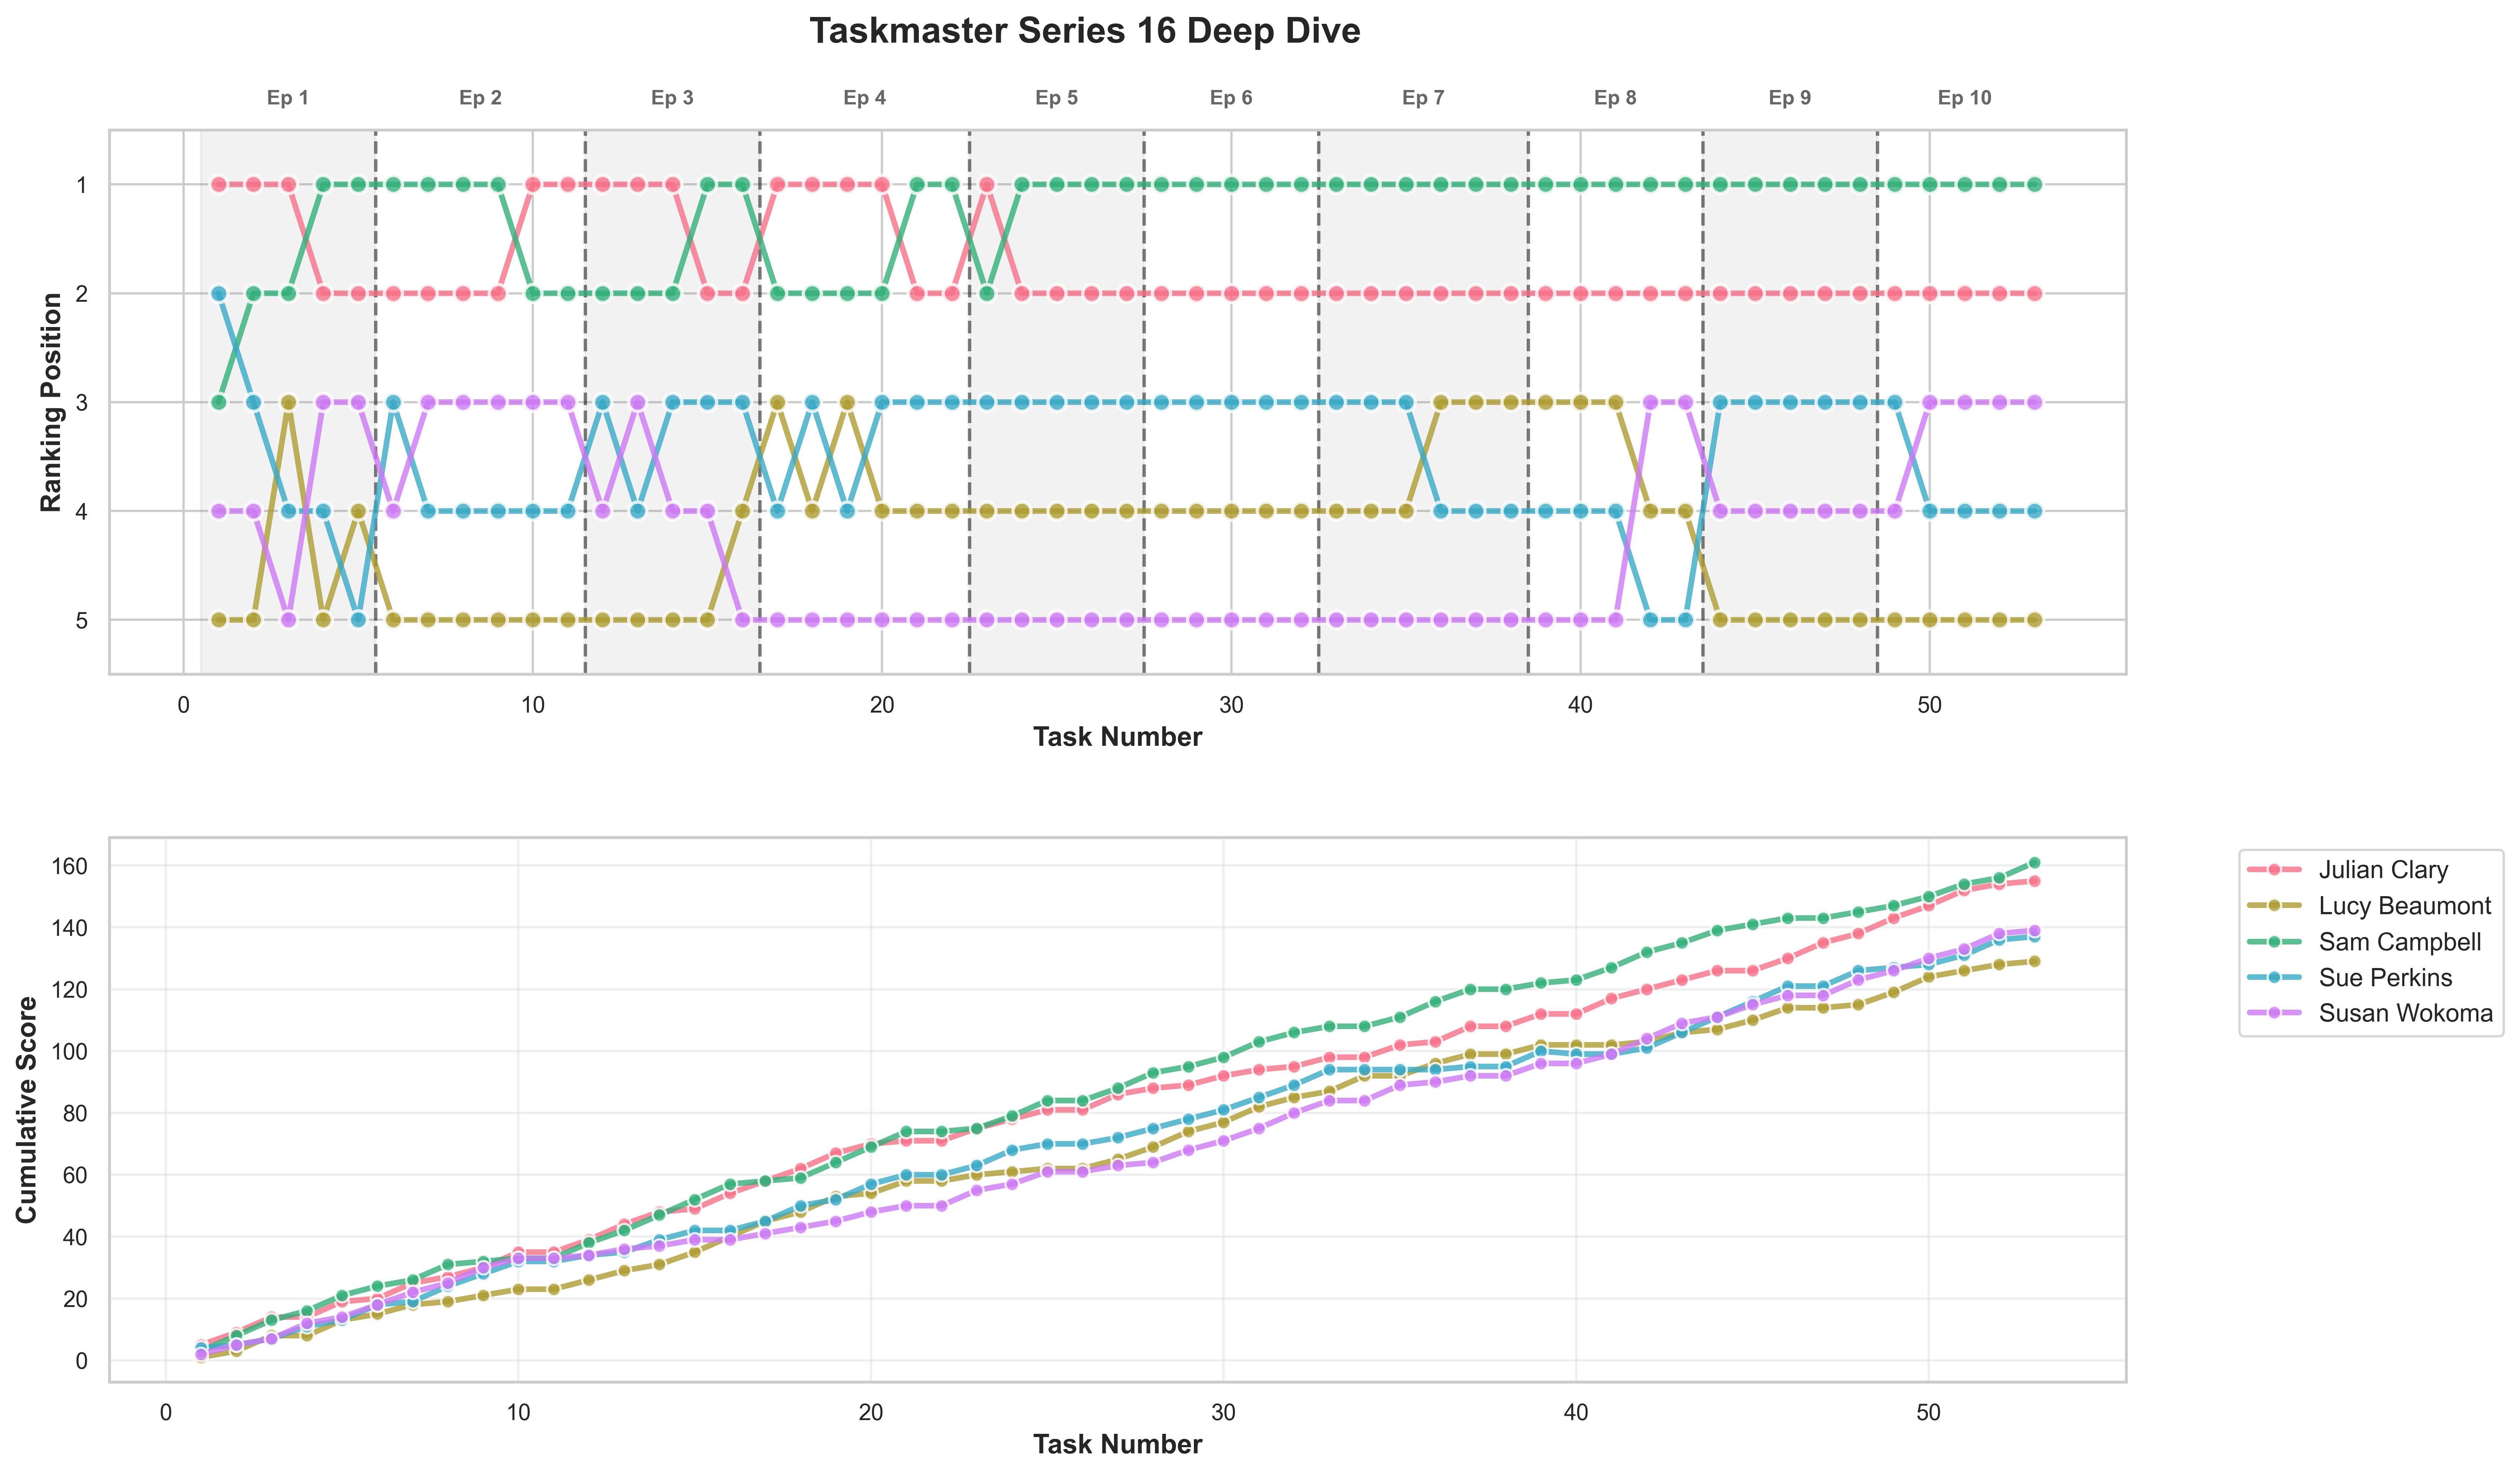
\includegraphics[width=\linewidth]{figures/supplementary/series_16_deep_dive.png}
\end{figure}
\FloatBarrier
\clearpage

\begin{figure}[!h]
\centering
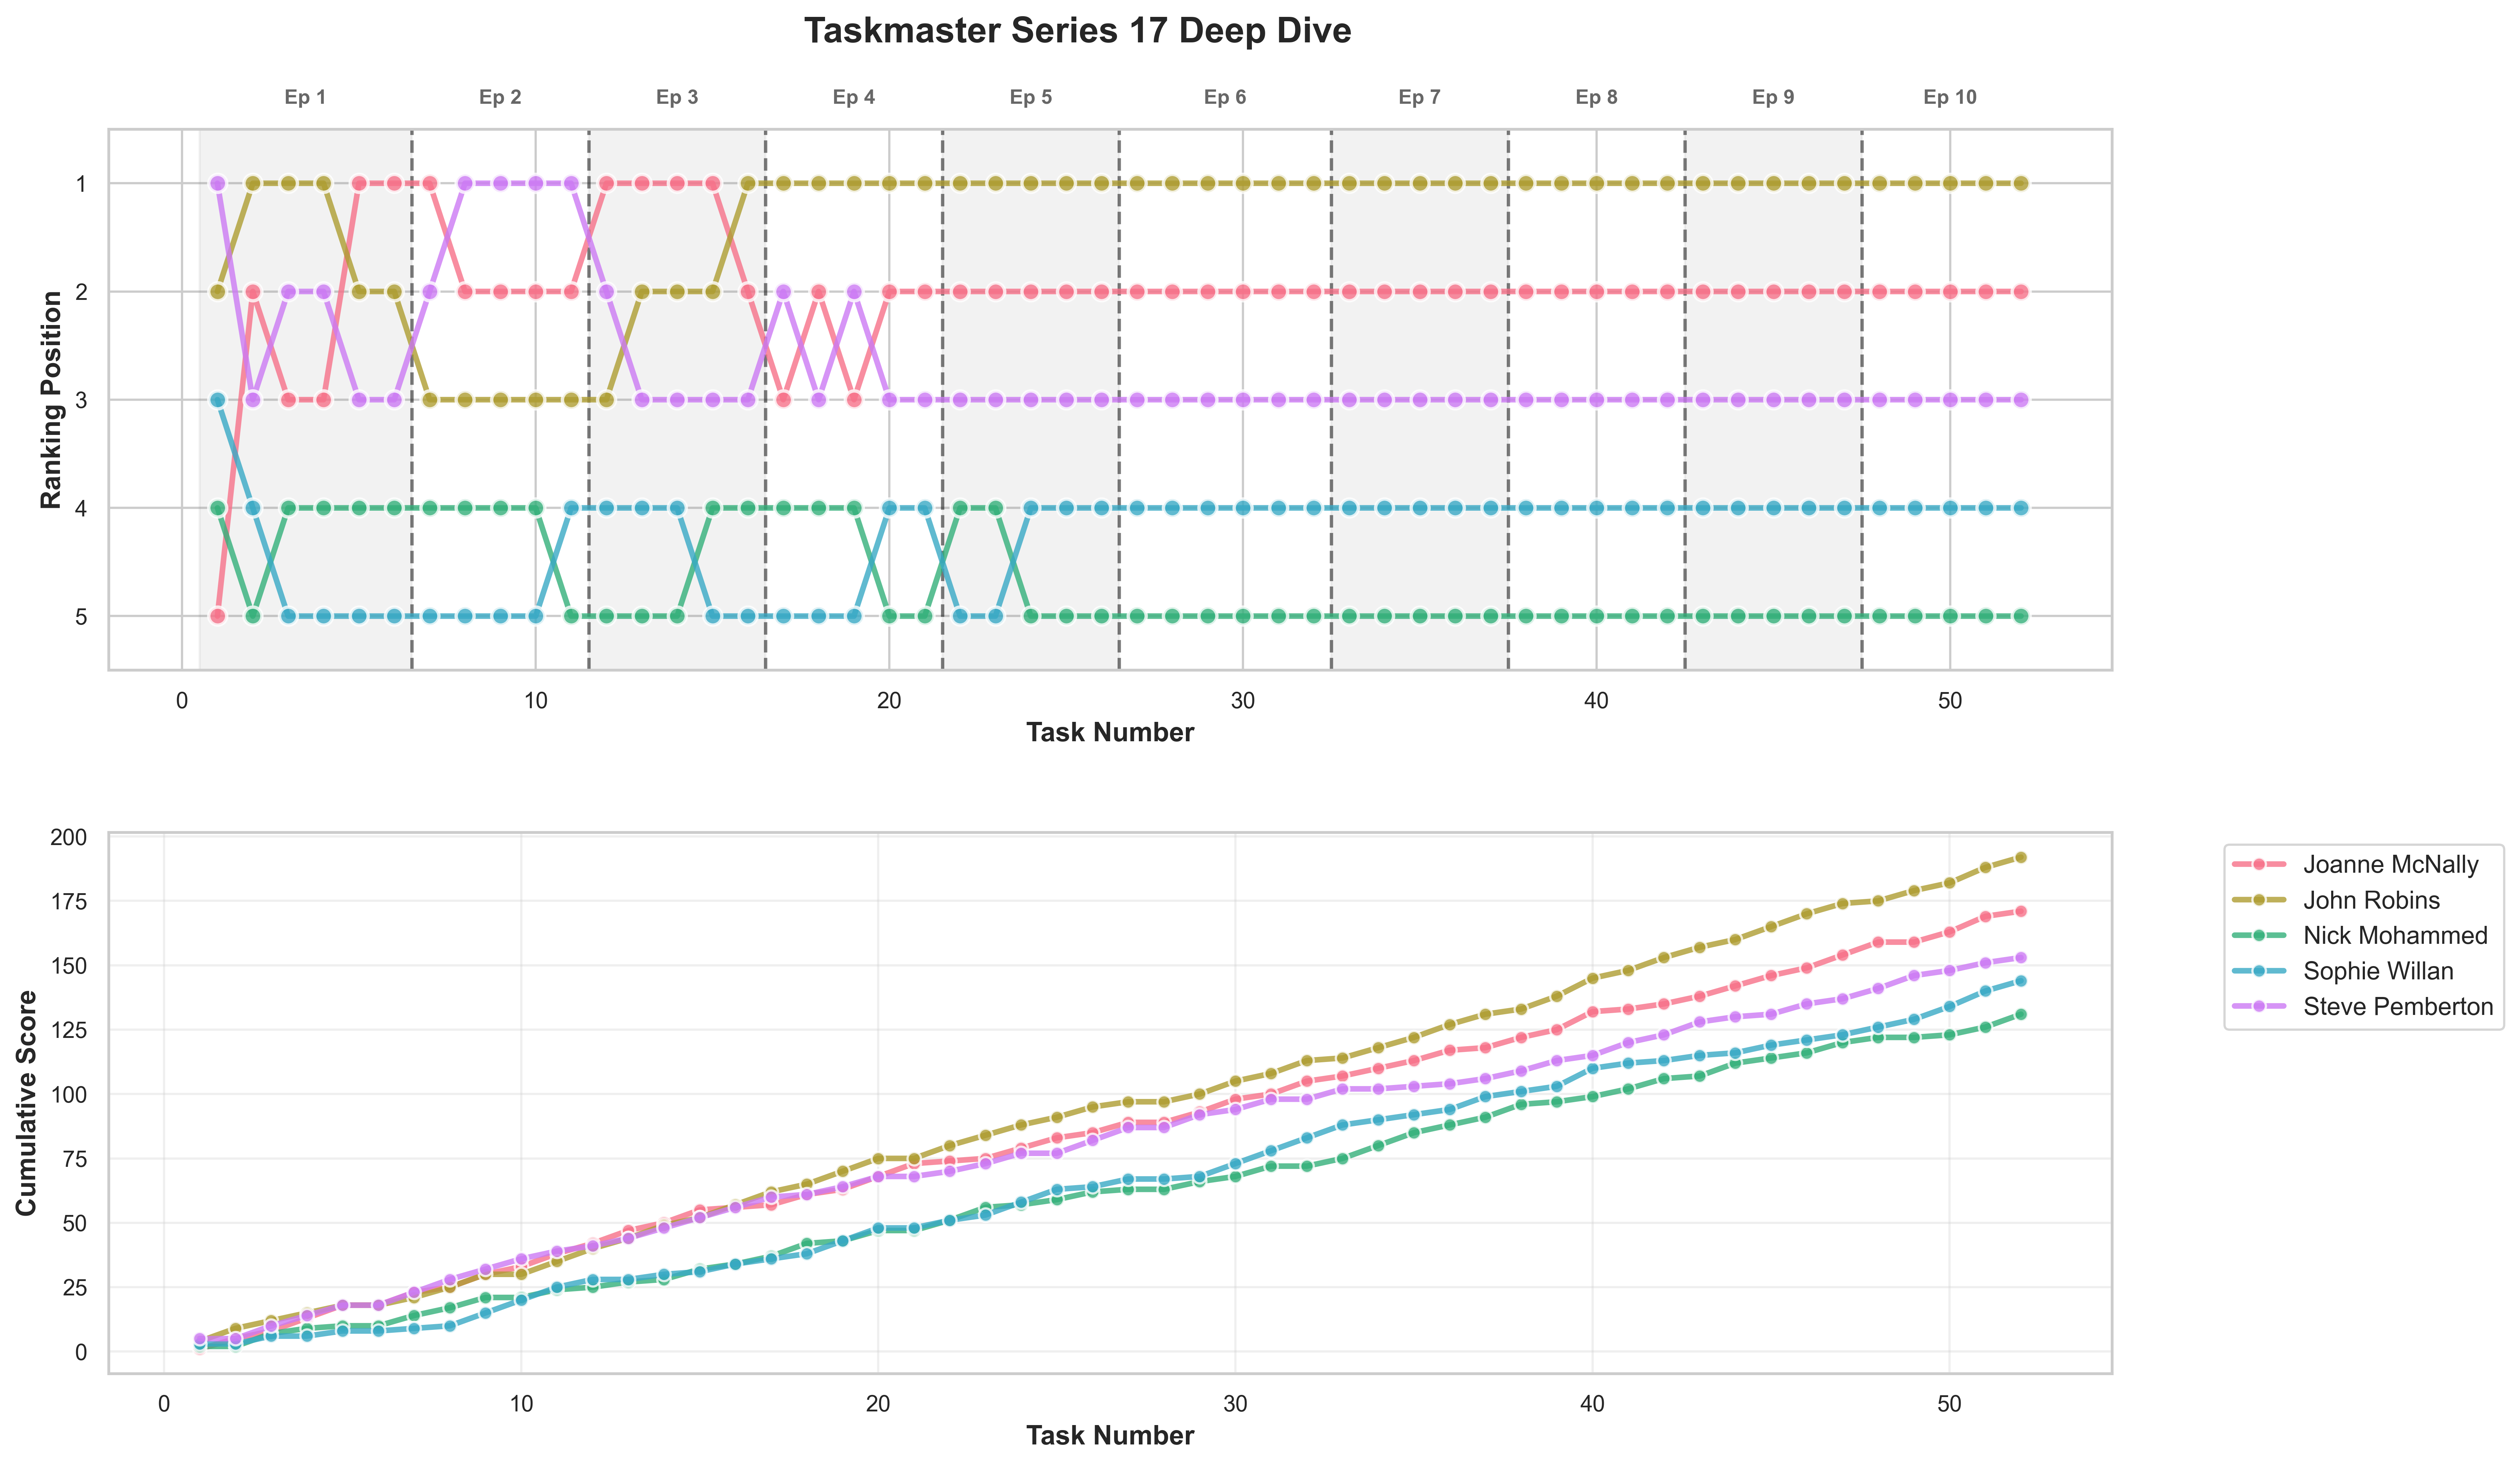
\includegraphics[width=\linewidth]{figures/supplementary/series_17_deep_dive.png}
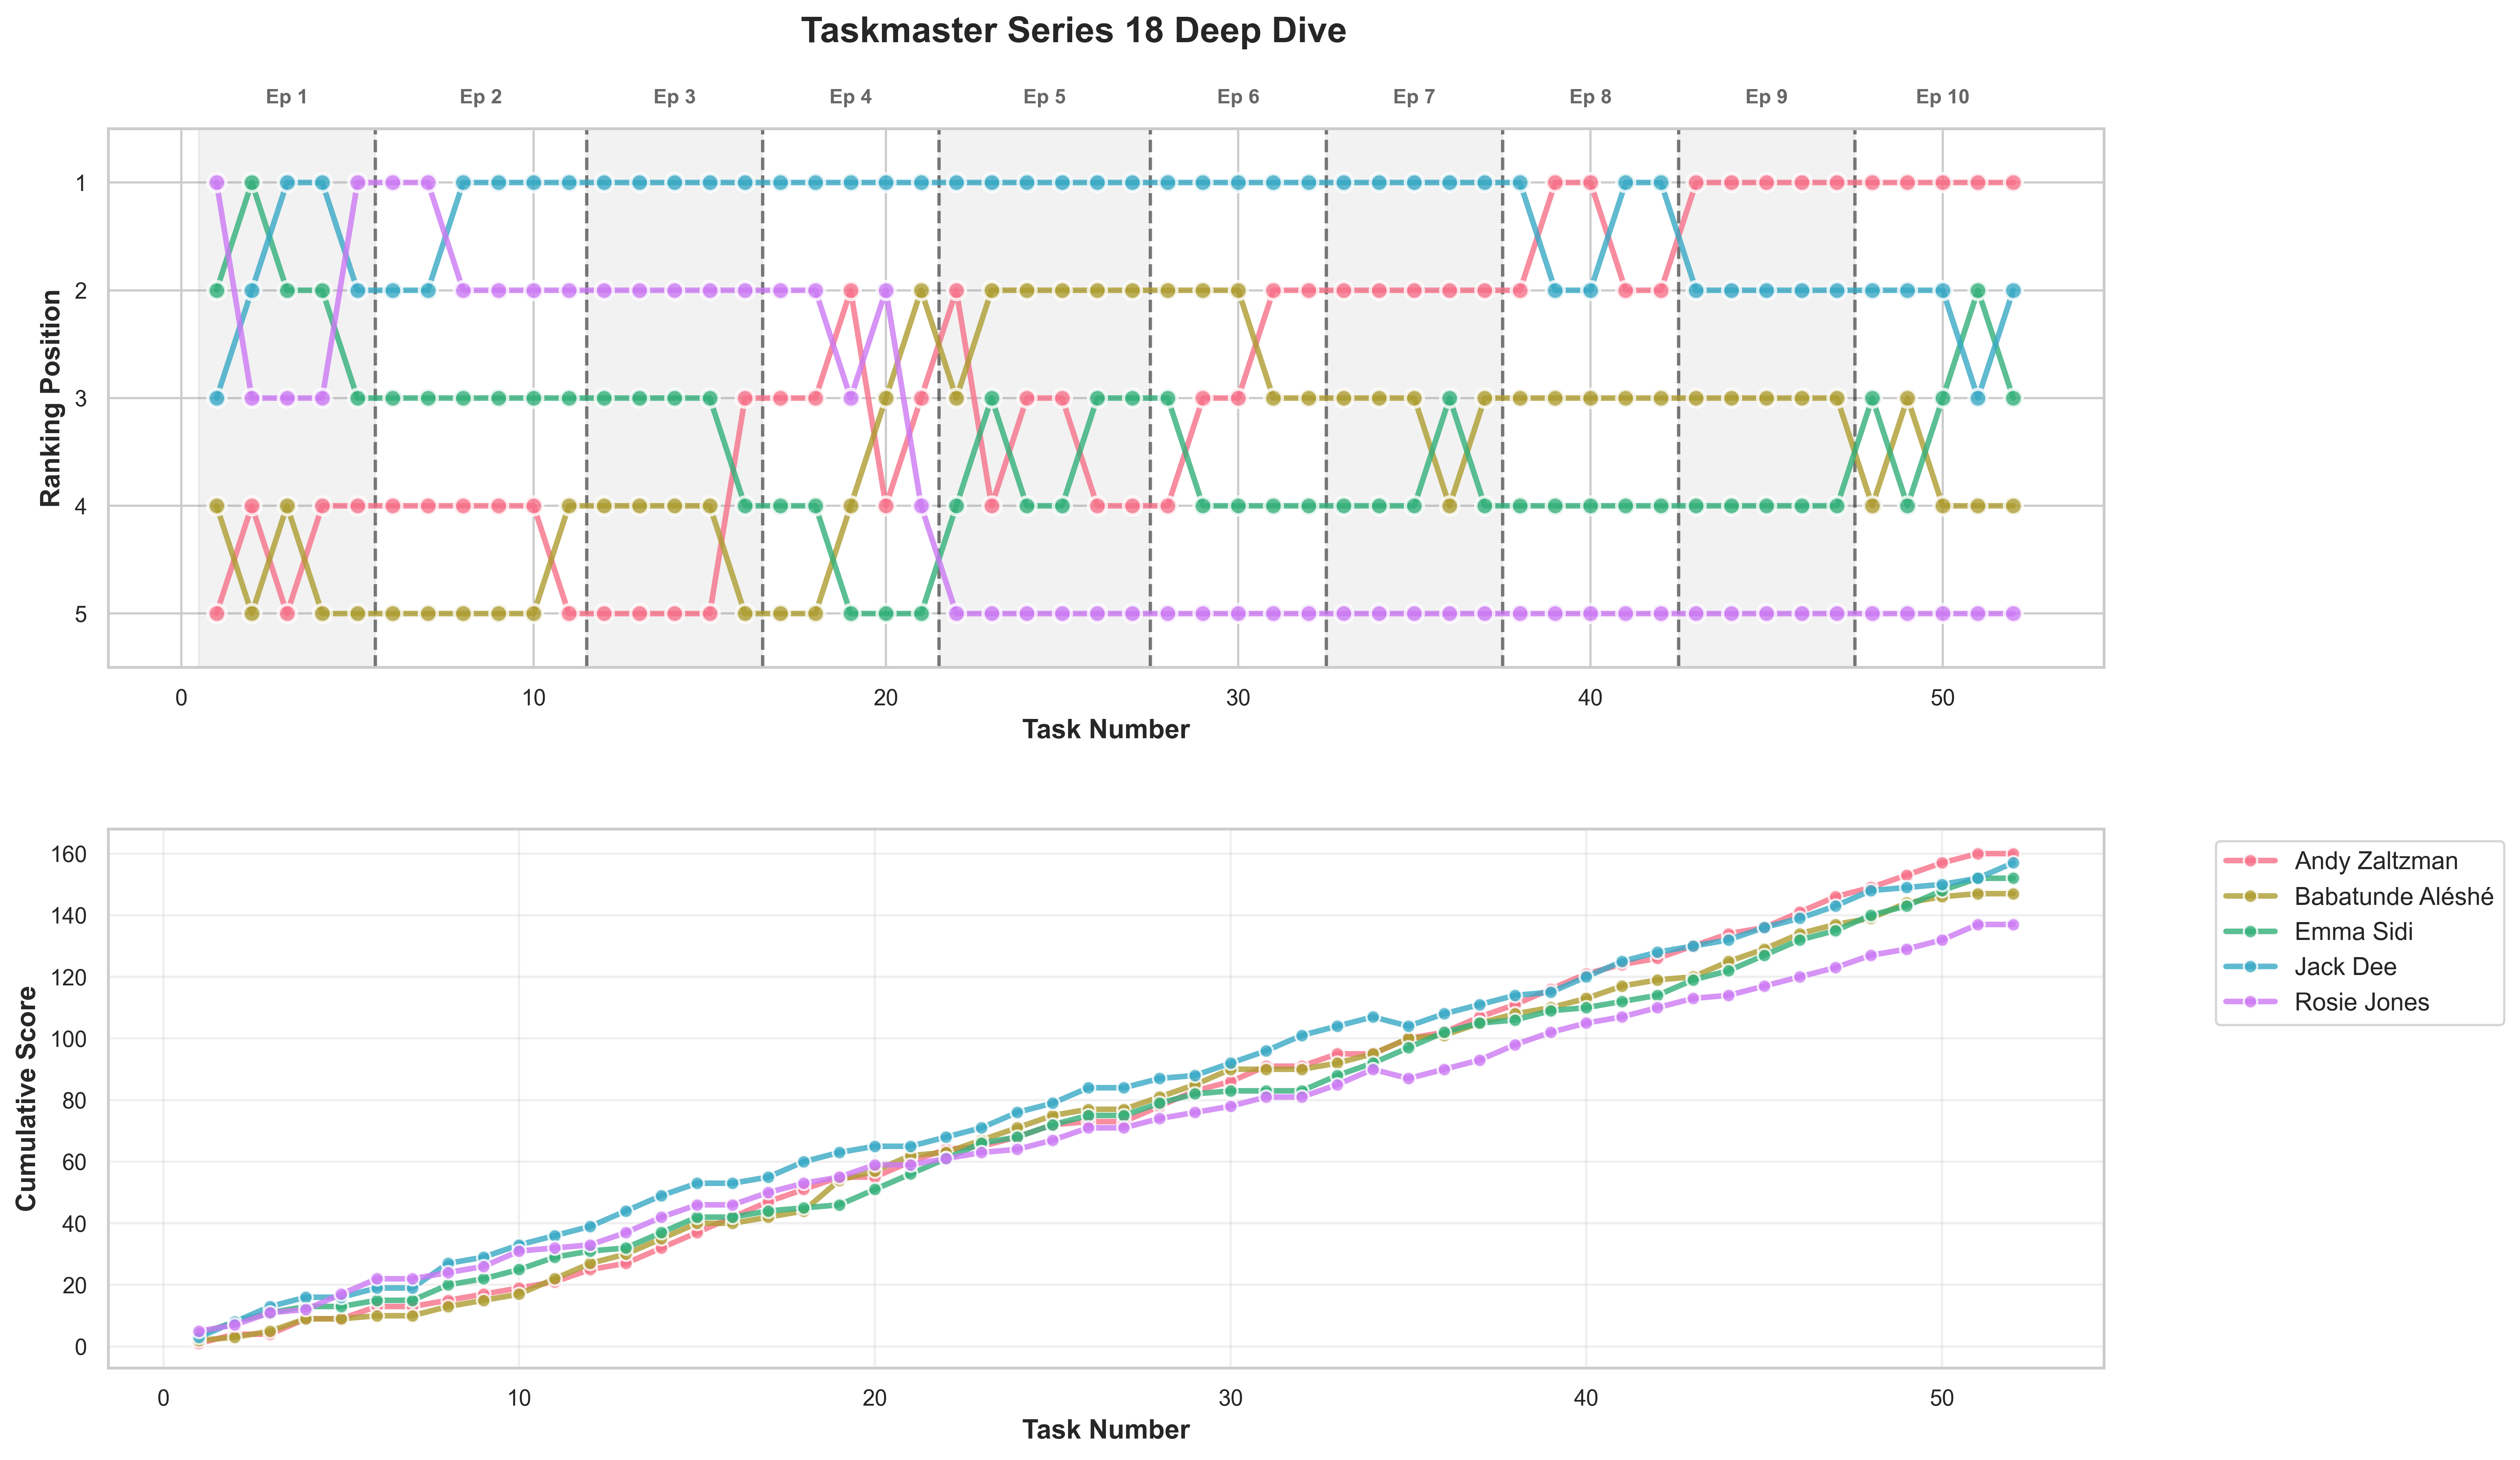
\includegraphics[width=\linewidth]{figures/supplementary/series_18_deep_dive.png}
\end{figure}
\FloatBarrier
\clearpage

\end{document} 